\documentclass[12pt,longbibliography]{article}
\usepackage[utf8]{inputenc}
\usepackage[T1]{fontenc}
\usepackage[catalan]{babel}
\usepackage[a4paper, margin=2.7cm]{geometry}

\usepackage{amsmath, amsthm, amsfonts, amssymb}
\newtheorem{thm}{Theorem}[section]
\newtheorem{cor}[thm]{Corollary}
\newtheorem{lem}[thm]{Lemma}
\newtheorem{prop}[thm]{Proposition}
\theoremstyle{definition}
\newtheorem{defn}[thm]{Definition}
\theoremstyle{remark}
\newtheorem{rem}[thm]{Remark}

\usepackage{mathrsfs} 
\usepackage[colorlinks=true,linkcolor=blue,citecolor=blue,urlcolor=blue,breaklinks]{hyperref}

\usepackage{bbm} 

\usepackage{hyperref}
\usepackage{graphicx}
\graphicspath{ {Imatges portada/} }

\title{Big Query}
\author{Anna Salazar}

\renewcommand{\contentsname}{Índex}
\renewcommand{\figurename}{Figura}
\renewcommand{\tablename}{Taula}

\begin{document}
\begin{titlepage}
\maketitle

\vspace{140mm}

\par
\raisebox{-.5\height}{
\includegraphics[width=6cm]{fme}}%
\hfill
\raisebox{-.5\height}{
\includegraphics[width=6cm]{UB}}%
\par

\end{titlepage}

\tableofcontents

\pagebreak

\pagenumbering{arabic}

\section{Què és BigQuery?}

BigQuery és un motor d’anàlisi de macrodades (\textit{Big Data}) que permet executar consultes SQL al núvol sobre les dades emmagatzemades en aquest, sense importar el volum de les dades ni el tipus de consultes que es volen fer. El motor de consulta és capaç de treballar sobre terabytes de dades en qüestió de segons, i sobre petabytes en pocs minuts. Avui en dia, les empreses estan adoptant cada cop més la presa de decisions basades en dades i fomentant una cultura oberta en la qual les dades no estan aïllades dins dels departaments. BigQuery, en proporcionar els mitjans tecnològics per a promoure un canvi cultural cap a l’agilitat i l’obertura, realitza un paper molt important en l’augment del ritme de la innovació.

\vspace{2mm}

Treballar amb dades a BigQuery implica 3 aspectes principals: l’emmagatzemament, la incorporació de les dades i la consulta d’aquestes, Google s’encarrega de tota la resta. Com BigQuery és un servei totalment gestionat, no és necessari configurar ni instal·lar res en el nostre ordinador i, pel mateix motiu, no necessitem un administrador de la base de dades. Simplement, podem entrar en el nostre projecte de Google Cloud des del mateix navegador i començar a analitzar.

\vspace{2mm}

Pel que fa a l’emmagatzemament, les dades es guarden en una taula estructurada, la qual cosa significa que es pot utilitzar SQL estàndard per a facilitar la consulta i l’anàlisi de dades. BigQuery és perfecta pel \textit{Big Data} perquè gestiona tot aquest emmagatzemament i està proveïda d’operacions d’escalabilitat que funcionen de forma automàtica sense que l’usuari s’hagi d’involucrar,  per la qual cosa mai haurem de preocupar-nos per la grandària de les dades amb els quals treballem. Part de la consideració de disseny darrere de BigQuery és animar als usuaris a centrar-se en els coneixements en lloc de la infraestructura. Quan s’introdueixen les dades a BigQuery no és necessari pensar en els diferents tipus d’emmagatzemament, ni en els seus avantatges pel que fa a velocitat i cost; l’emmagatzemament està totalment gestionat.

\vspace{2mm}
\noindent
Per a més informació sobre BigQuery, es pot consultar la pàgina de \href{https://cloud.google.com/bigquery/docs/introduction}{Google Cloud}.

\subsection{Per què hauríem d'utilitzar BigQuery en lloc d'altres eines?}

Una de les característiques més rellevants que presenta BigQuery és que es tracta d'una plataforma sense servidor, és a dir, que els servidors s'executen en segon pla, sense la intervenció de l'usuari. A més, presenta una alta disponibilitat, la qual cosa es tradueix en que no cal preocupar-se per la caiguda dels servidors, ja que la plataforma s'encarrega d'això. Finalment, BigQuery també té propietats d'escalabilitat automàtica que fan possible gestionar fins a petabytes de dades. Aquestes característiques no estan disponibles a la majoria de plataformes d'emmagatzemament de dades tradicionals, i fan destacar BigQuery entre moltes.

\vspace{2mm}

Com en molts altres magatzems de dades, BigQuery és capaç de treballar amb moltes fonts de dades diferents. Podem pujar les dades des del nostre propi sistema d'arxius, de Google Cloud Storage, de Google Drive i de moltes fonts més. Després de fer-ho, es poden consultar aquestes dades utilitzant SQL estàndard o SQL heretat, el rendiment en qualsevol cas és excel·lent. Els resultats de les consultes solen emmagatzemar-se en la memòria cau durant 24 hores, de manera que les següents execucions d'aquesta consulta només hauran d'obtenir les dades de la memòria cau en lloc de fer-ho del disc. 


\pagebreak

\section{Creació i treball amb conjunts de dades i taules}

\subsection{Configuració de la Plataforma de Google Cloud (GCP)}

\graphicspath{ {BigQuery/Imatges tutorial/} }

Per utilitzar aquesta eina d’anàlisi només ens caldrà crear un compte a Google Cloud i treballar a la zona de proves que ofereix Google per operar de forma gratuïta.
Per fer servir la zona de proves (\textit{Sandbox}) seguirem els passos següents: 

\vspace{2mm}

1. En primer lloc, ens dirigim a la interfície d’usuari (UI) de \href{https://console.cloud.google.com}{BigQuery}. Des d'aquesta interfície es poden realitzar la majoria de les operacions.

\vspace{2mm}

2. Accedim al nostre compte de Google o creem un nou compte si encara no en tenim cap. Si és el primer cop que iniciem sessió a Google Cloud, haurem de marcar el país on som i acceptar les condicions de servei.

\vspace{2mm}

3. Un cop dins, podem veure com és l'espai de treball SQL. Hi ha una secció de l'Explorador a l'esquerra que ens permet navegar en projectes, conjunts de dades i taules. Per tal de fer servir la zona de proves, haurem de crear un projecte.

Introdueix un nom al teu projecte i fes clic a \textit{Create}. En el nostre cas, hem anomenat el projecte \verb|el_meu_projecte| (Figura ~\ref{fig:bq1}), i treballarem sobre aquest per il·lustrar el funcionament de la plataforma.

\vspace{2mm}
\begin{figure}[h!]
\par
\raisebox{-.5\height}{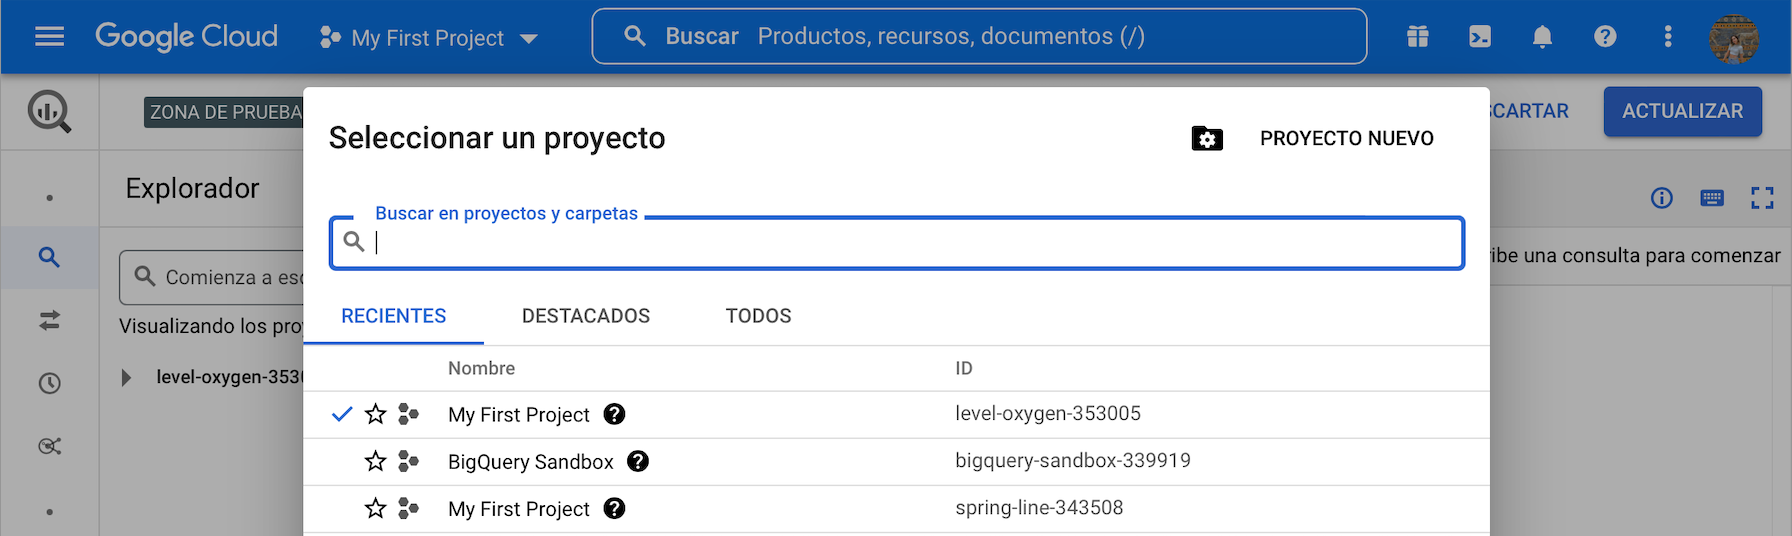
\includegraphics[width=7.25cm]{bq1}}%
\hfill
\raisebox{-.5\height}{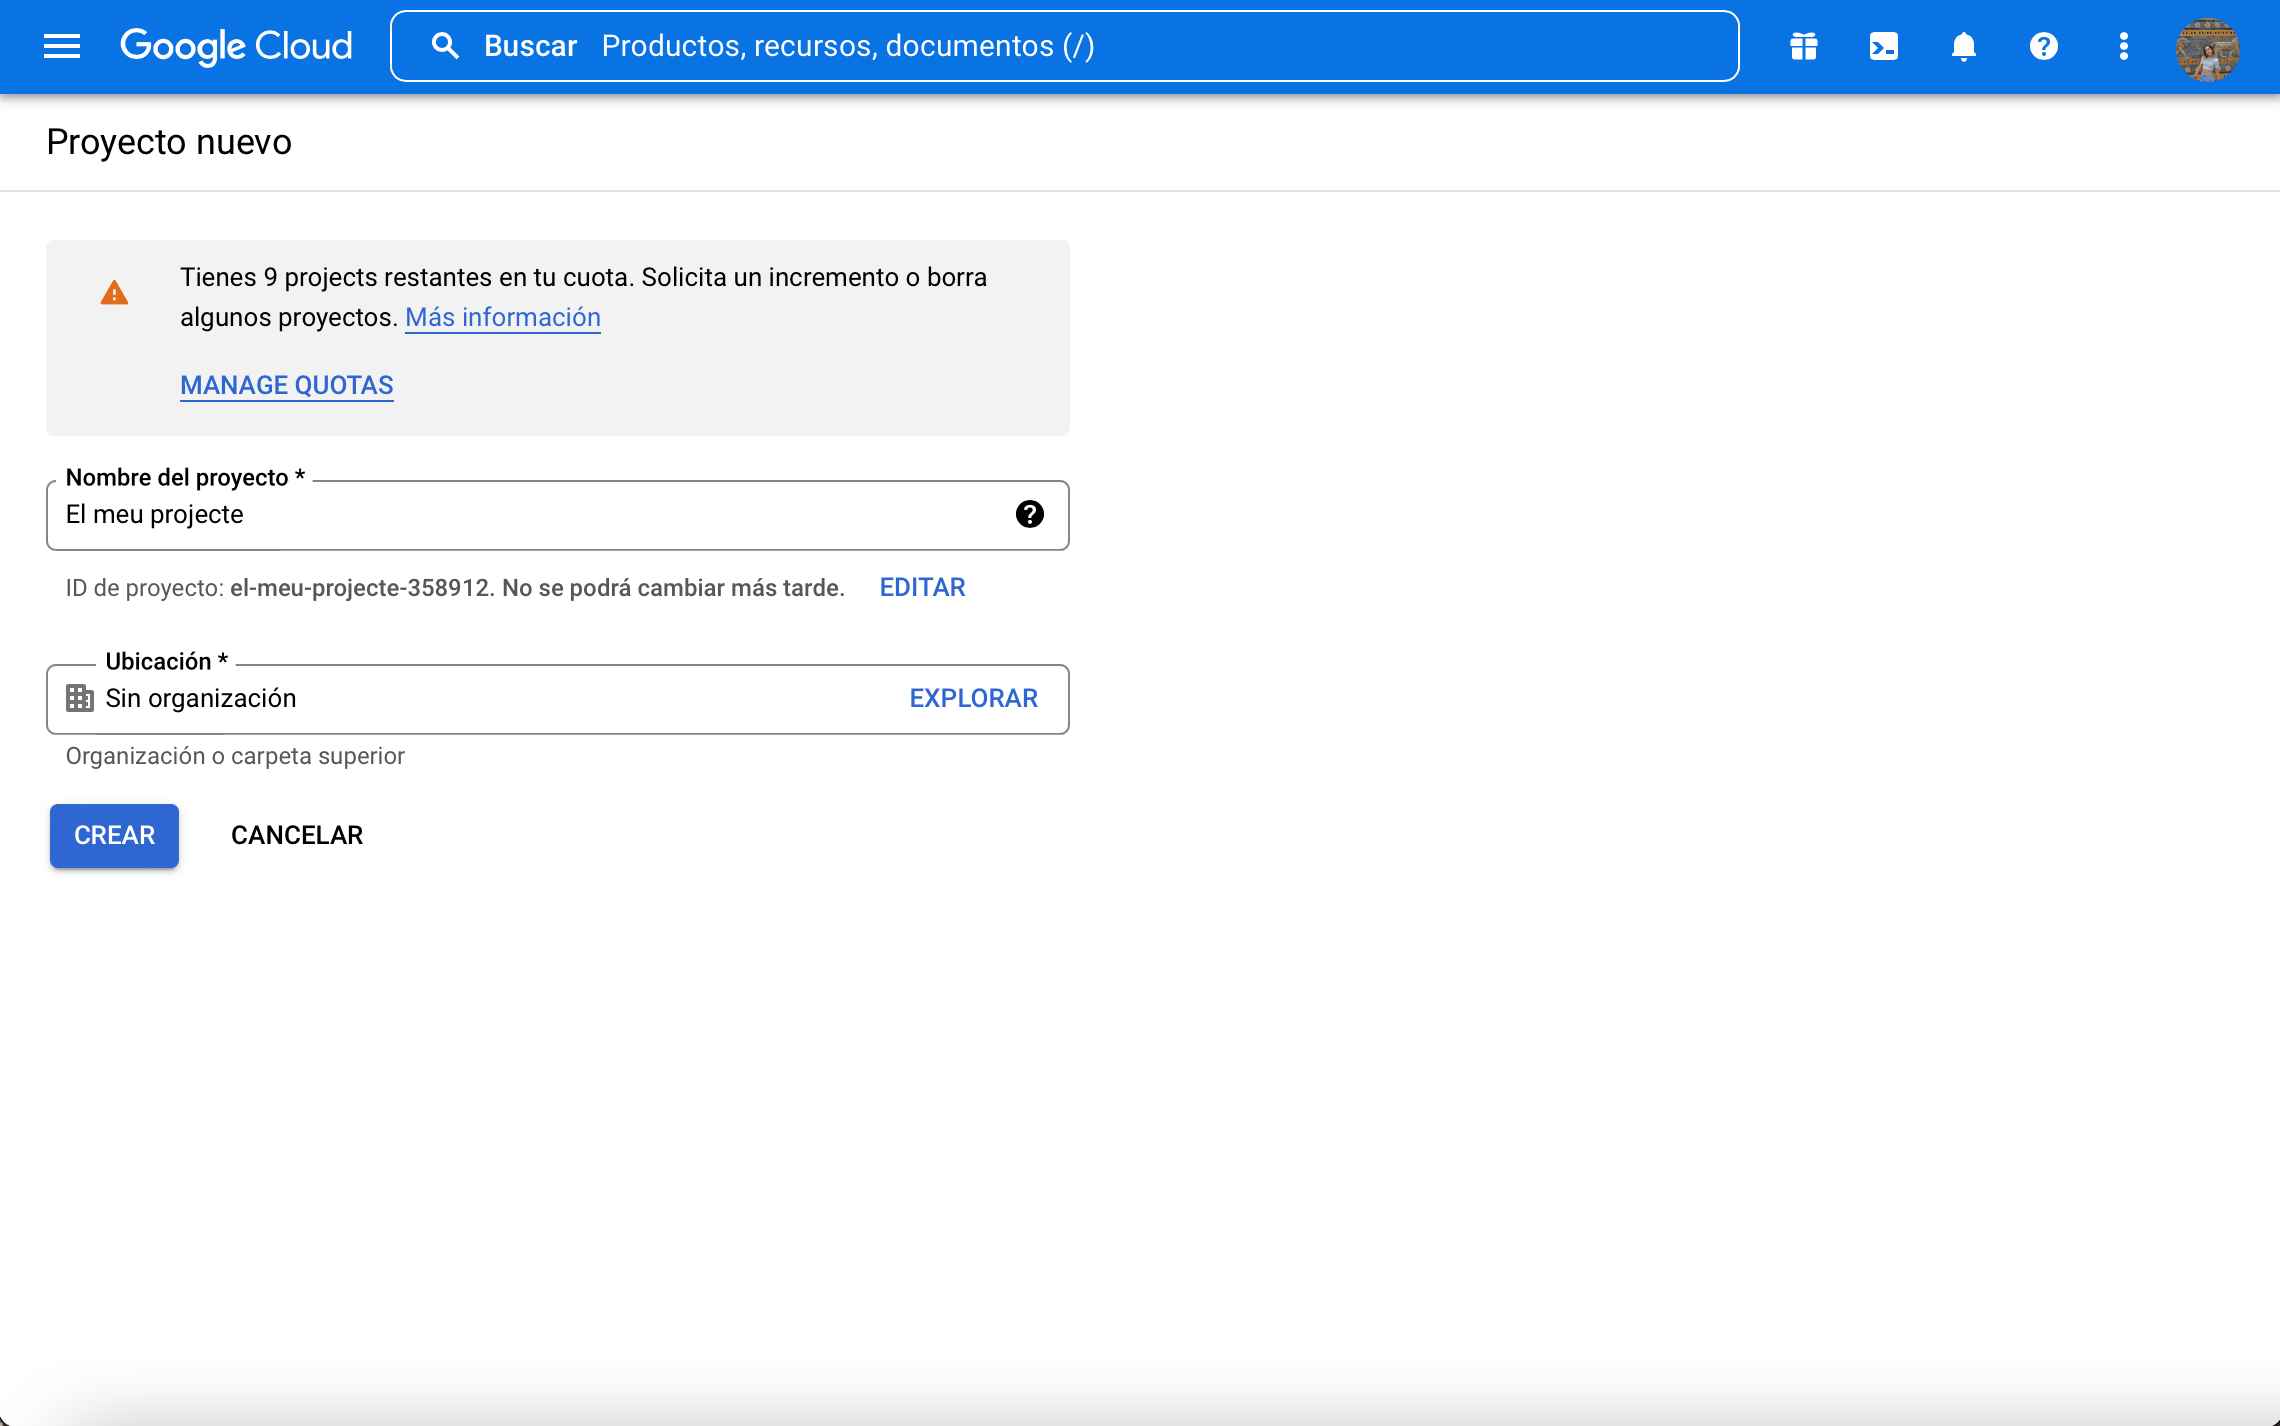
\includegraphics[width=7.25cm]{bq2}}%
\par
\caption{Creació d'un projecte}
\label{fig:bq1}
\end{figure}
\vspace{2mm}

4. Un cop creat el projecte, el navegador ens redirigeix a la interfície web de BigQuery.

\vspace{2mm}

5. Ara ja podrem carregar o consultar dades en el nostre projecte sense cap compte de facturació adjunta.

\subsubsection{Limitacions}

Això no obstant, per a l’ús de la zona de proves gratuïta que ofereix Google, haurem de tenir en compte un seguit de limitacions.

\vspace{2mm}

En primer lloc, ens trobem amb un màxim de 10 Gb d’emmagatzemament i 10 Tb de consulta al mes. Al llarg d’aquest projecte no utilitzarem un volum de dades més gran ni sobrepassarem el límit d’espai de consulta, però s’han de tenir en compte aquestes limitacions si l’objectiu és treballar amb el format gratuït.

\vspace{2mm}

A més, ens trobem que tots els conjunts de dades tenen el temps de caducitat de la taula per defecte establerta en seixanta dies. Per tant, totes les taules, vistes o particions de les taules caducaran automàticament passats els seixanta dies.

\vspace{2mm}

Una altra característica destacable és que els projectes de la zona de proves no són compatibles amb:

- La transmissió de dades

- Sentència de llenguatge de manipulació de dades (DML)

- Servei de transferència de dades de BigQuery

\subsection{Creació d'un conjunt de dades}

Ara que ja coneixem les limitacions de la plataforma i disposem d'un projecte en el qual crear un conjunt de dades, ha arribat el moment de crear un nou conjunt de dades dins d'aquest projecte. Es pot pensar en un conjunt de dades a BigQuery com una agrupació lògica de taules. Alhora, diferents conjunts de dades s'integren en un mateix projecte. 

\vspace{2mm}

Per a crear-ne un, només s'ha de desplegar el menú i triar l'opció de crear un nou conjunt de dades. Tot seguit hi ha diversos detalls per al conjunt de dades que es poden establir. En primer lloc, hi ha l'opció de canviar el projecte que l'encabirà. Això farà que aparegui un navegador on es podrà especificar el projecte. Una altra possibilitat serà escollir la ubicació de les dades. Això determina on s'aprovisionaran els recursos subjacents, com la computació i l'emmagatzematge, per al servei BigQuery. Les consideracions a l'hora de triar una ubicació inclouran el rendiment per als usuaris finals, l'alta disponibilitat i també qualsevol restricció d'auditoria o compliment. I, per últim, es pot establir un temps d'expiració per defecte per a les taules dins d'un conjunt de dades.

\vspace{2mm}
\begin{figure}[h!]
\par
\raisebox{-.5\height}{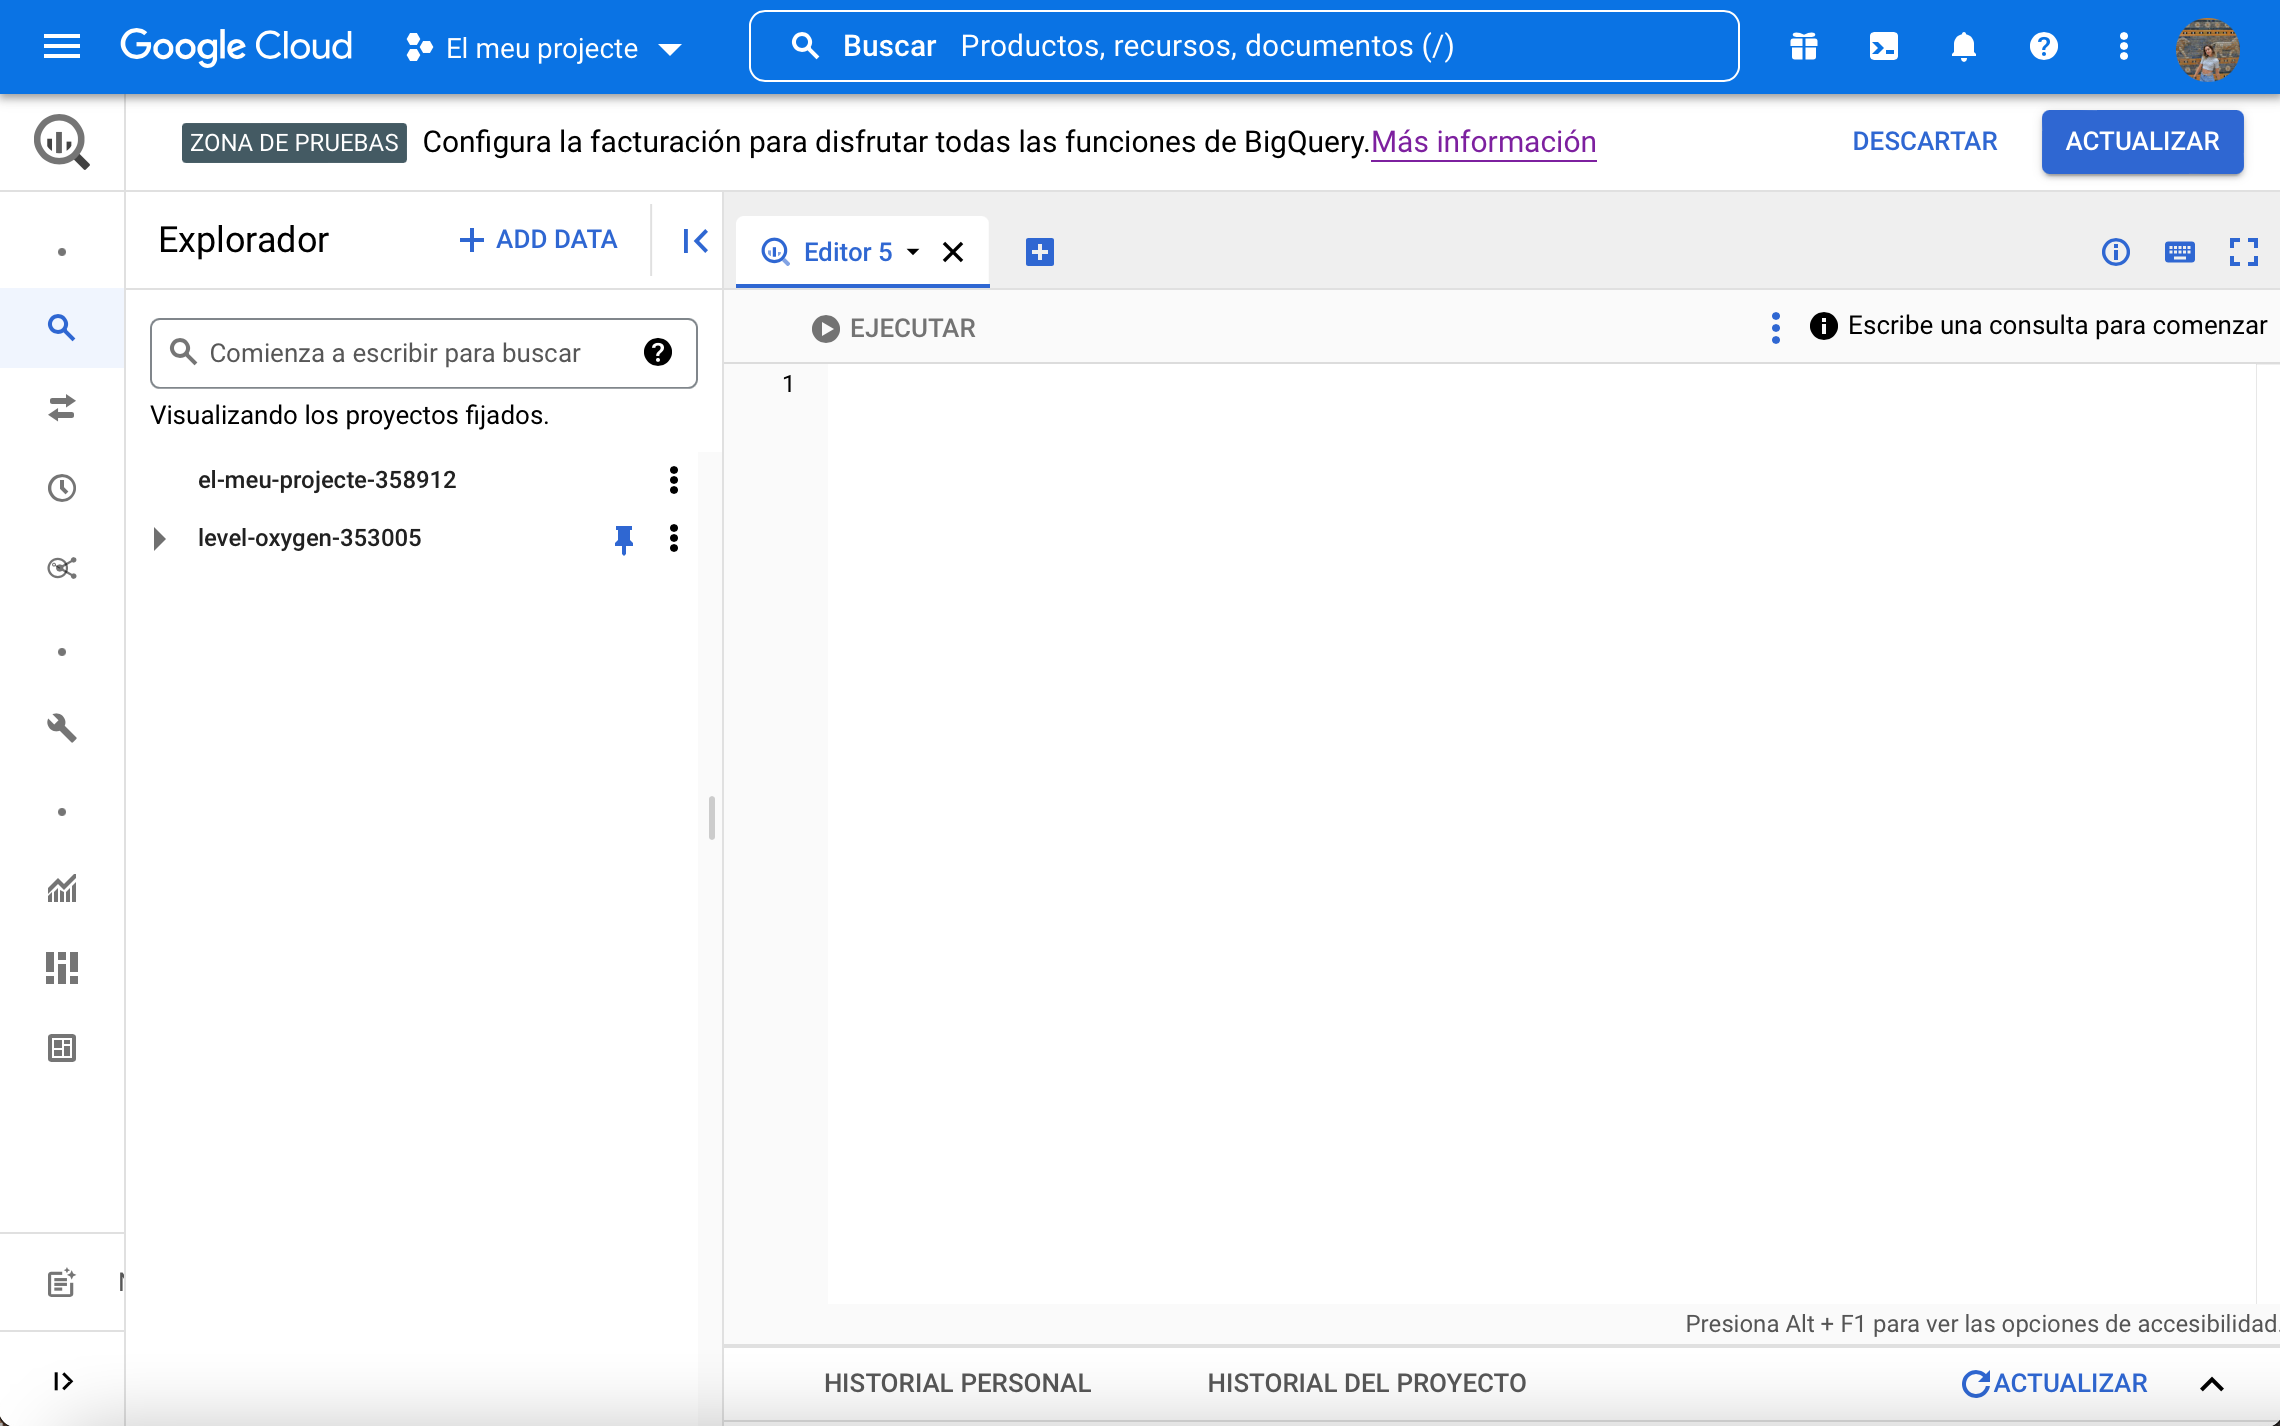
\includegraphics[width=7.25cm]{bq3}}%
\hfill
\raisebox{-.5\height}{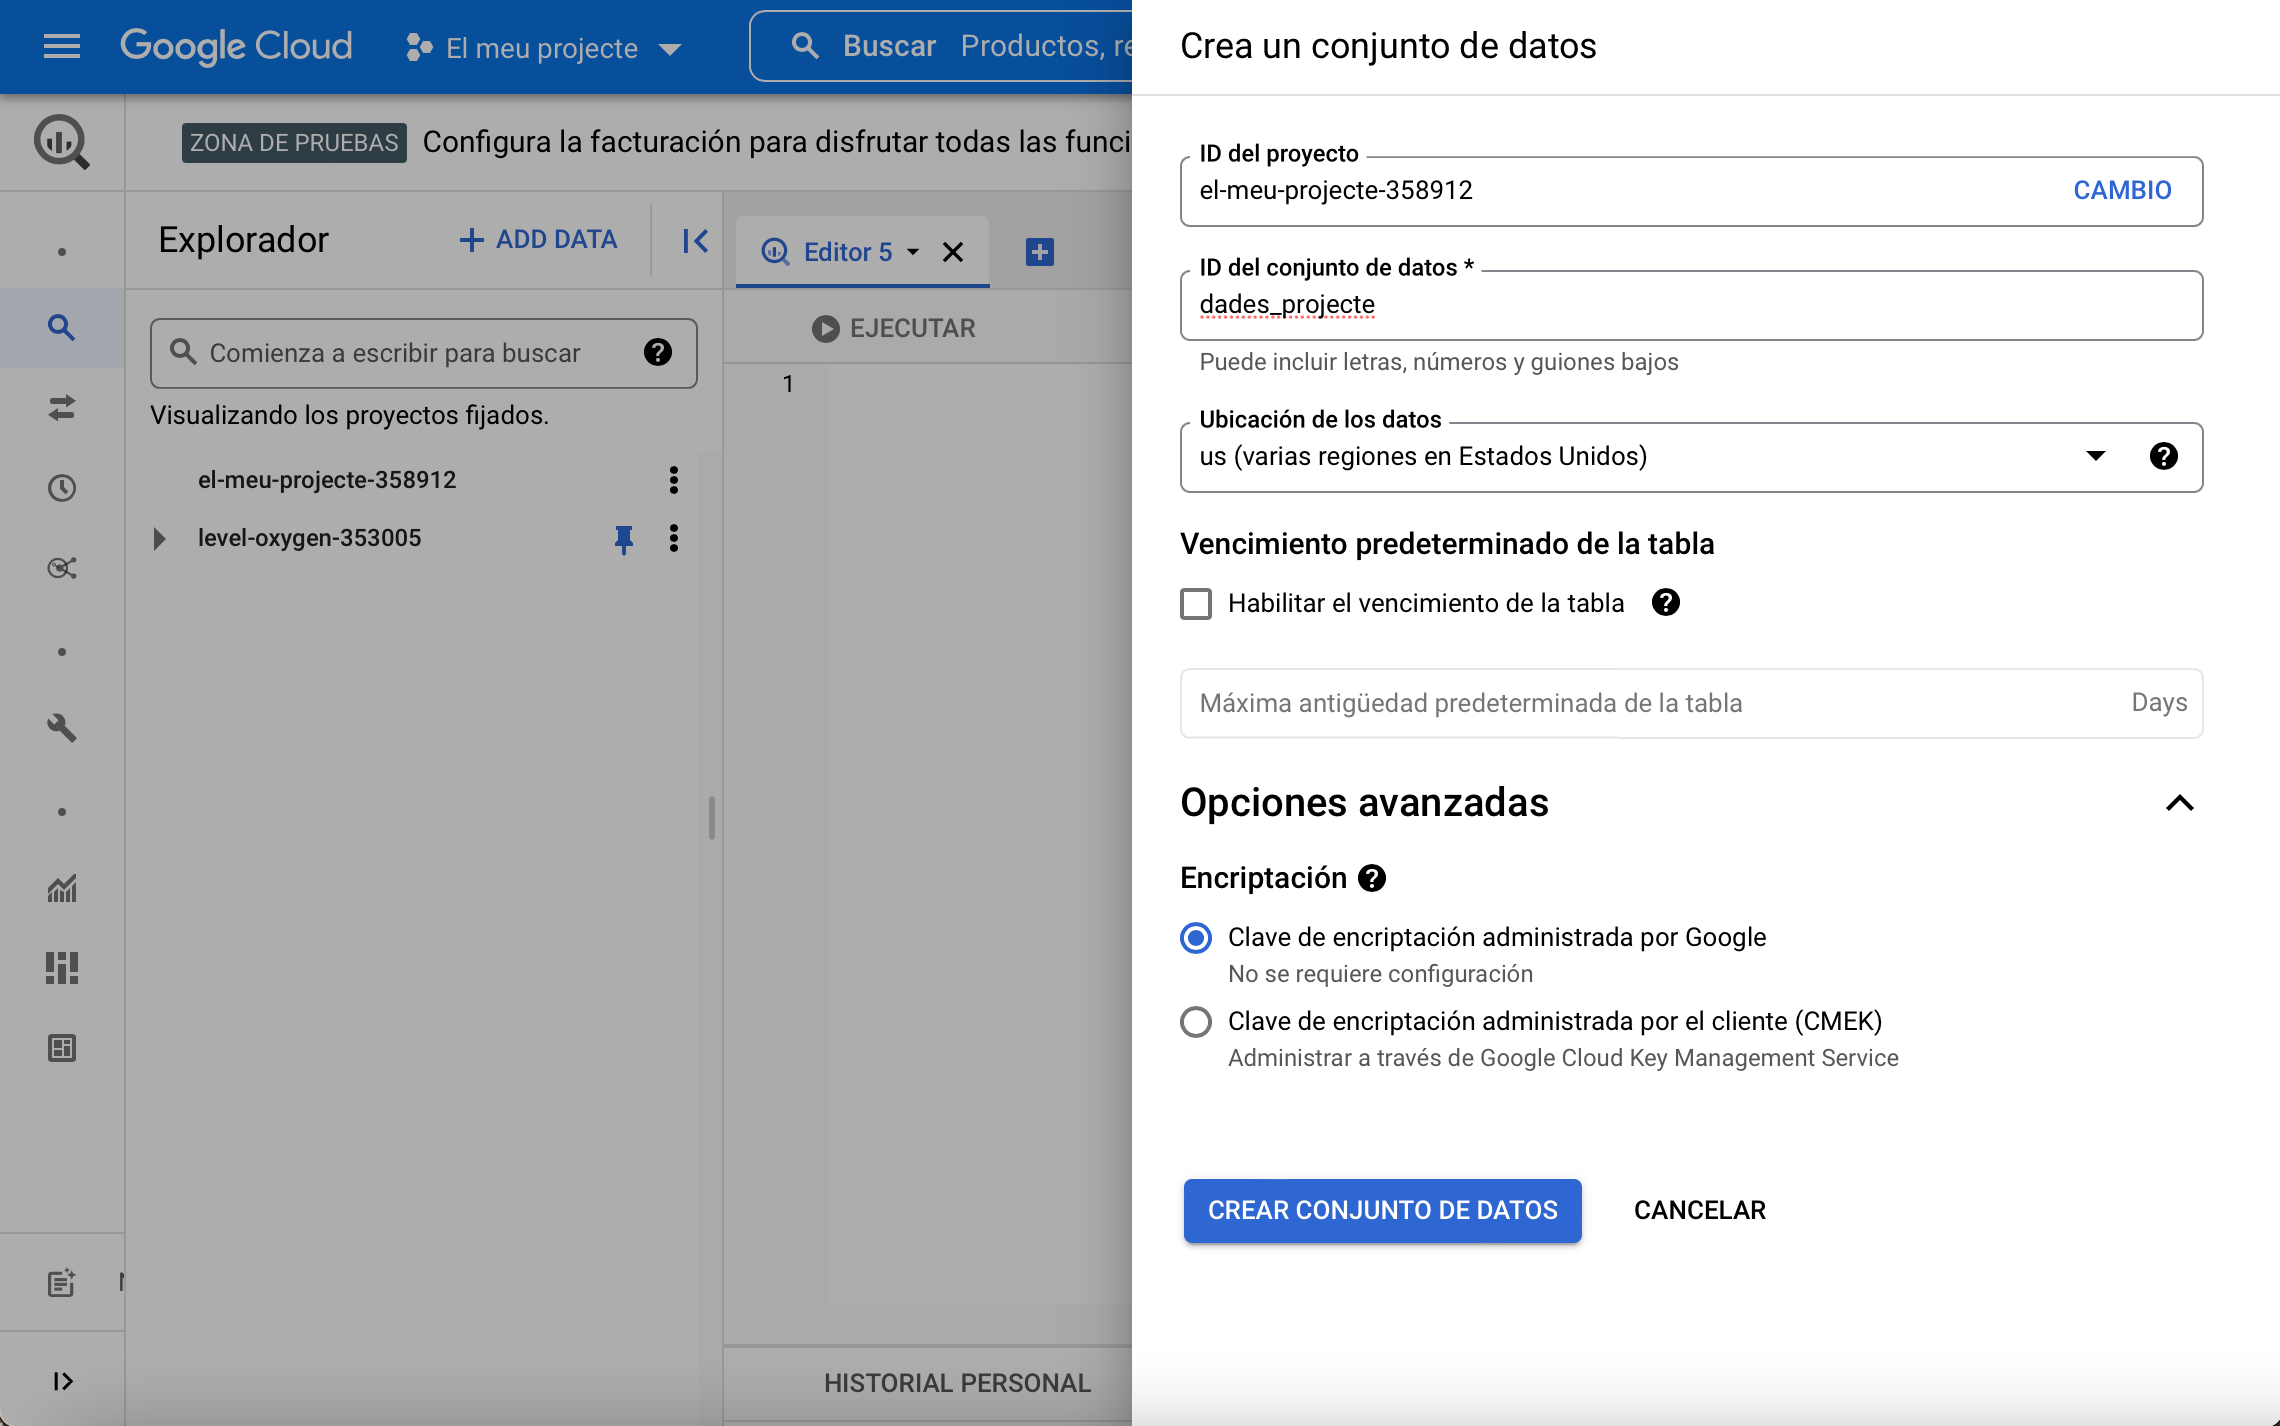
\includegraphics[width=7.25cm]{bq4}}%
\par
\caption{Creació d'un conjunt de dades}
\label{fig:bq3}
\end{figure}
\vspace{2mm}

Tal com es pot veure a la figura ~\ref{fig:bq3}, hem creat un nou conjunt de dades anomenat \verb|dades_projecte| que estarà ubicat en el projecte \verb|el_meu_projecte|, la ubicació de les dades l'hem posat a diverses regions dels Estats Units i, per últim, no hem habilitat un temps de venciment de la taula, sinó que per defecte BigQuery l'emmagatzemarà per seixanta dies.

\vspace{2mm}
\begin{figure}[h!]
\begin{center}
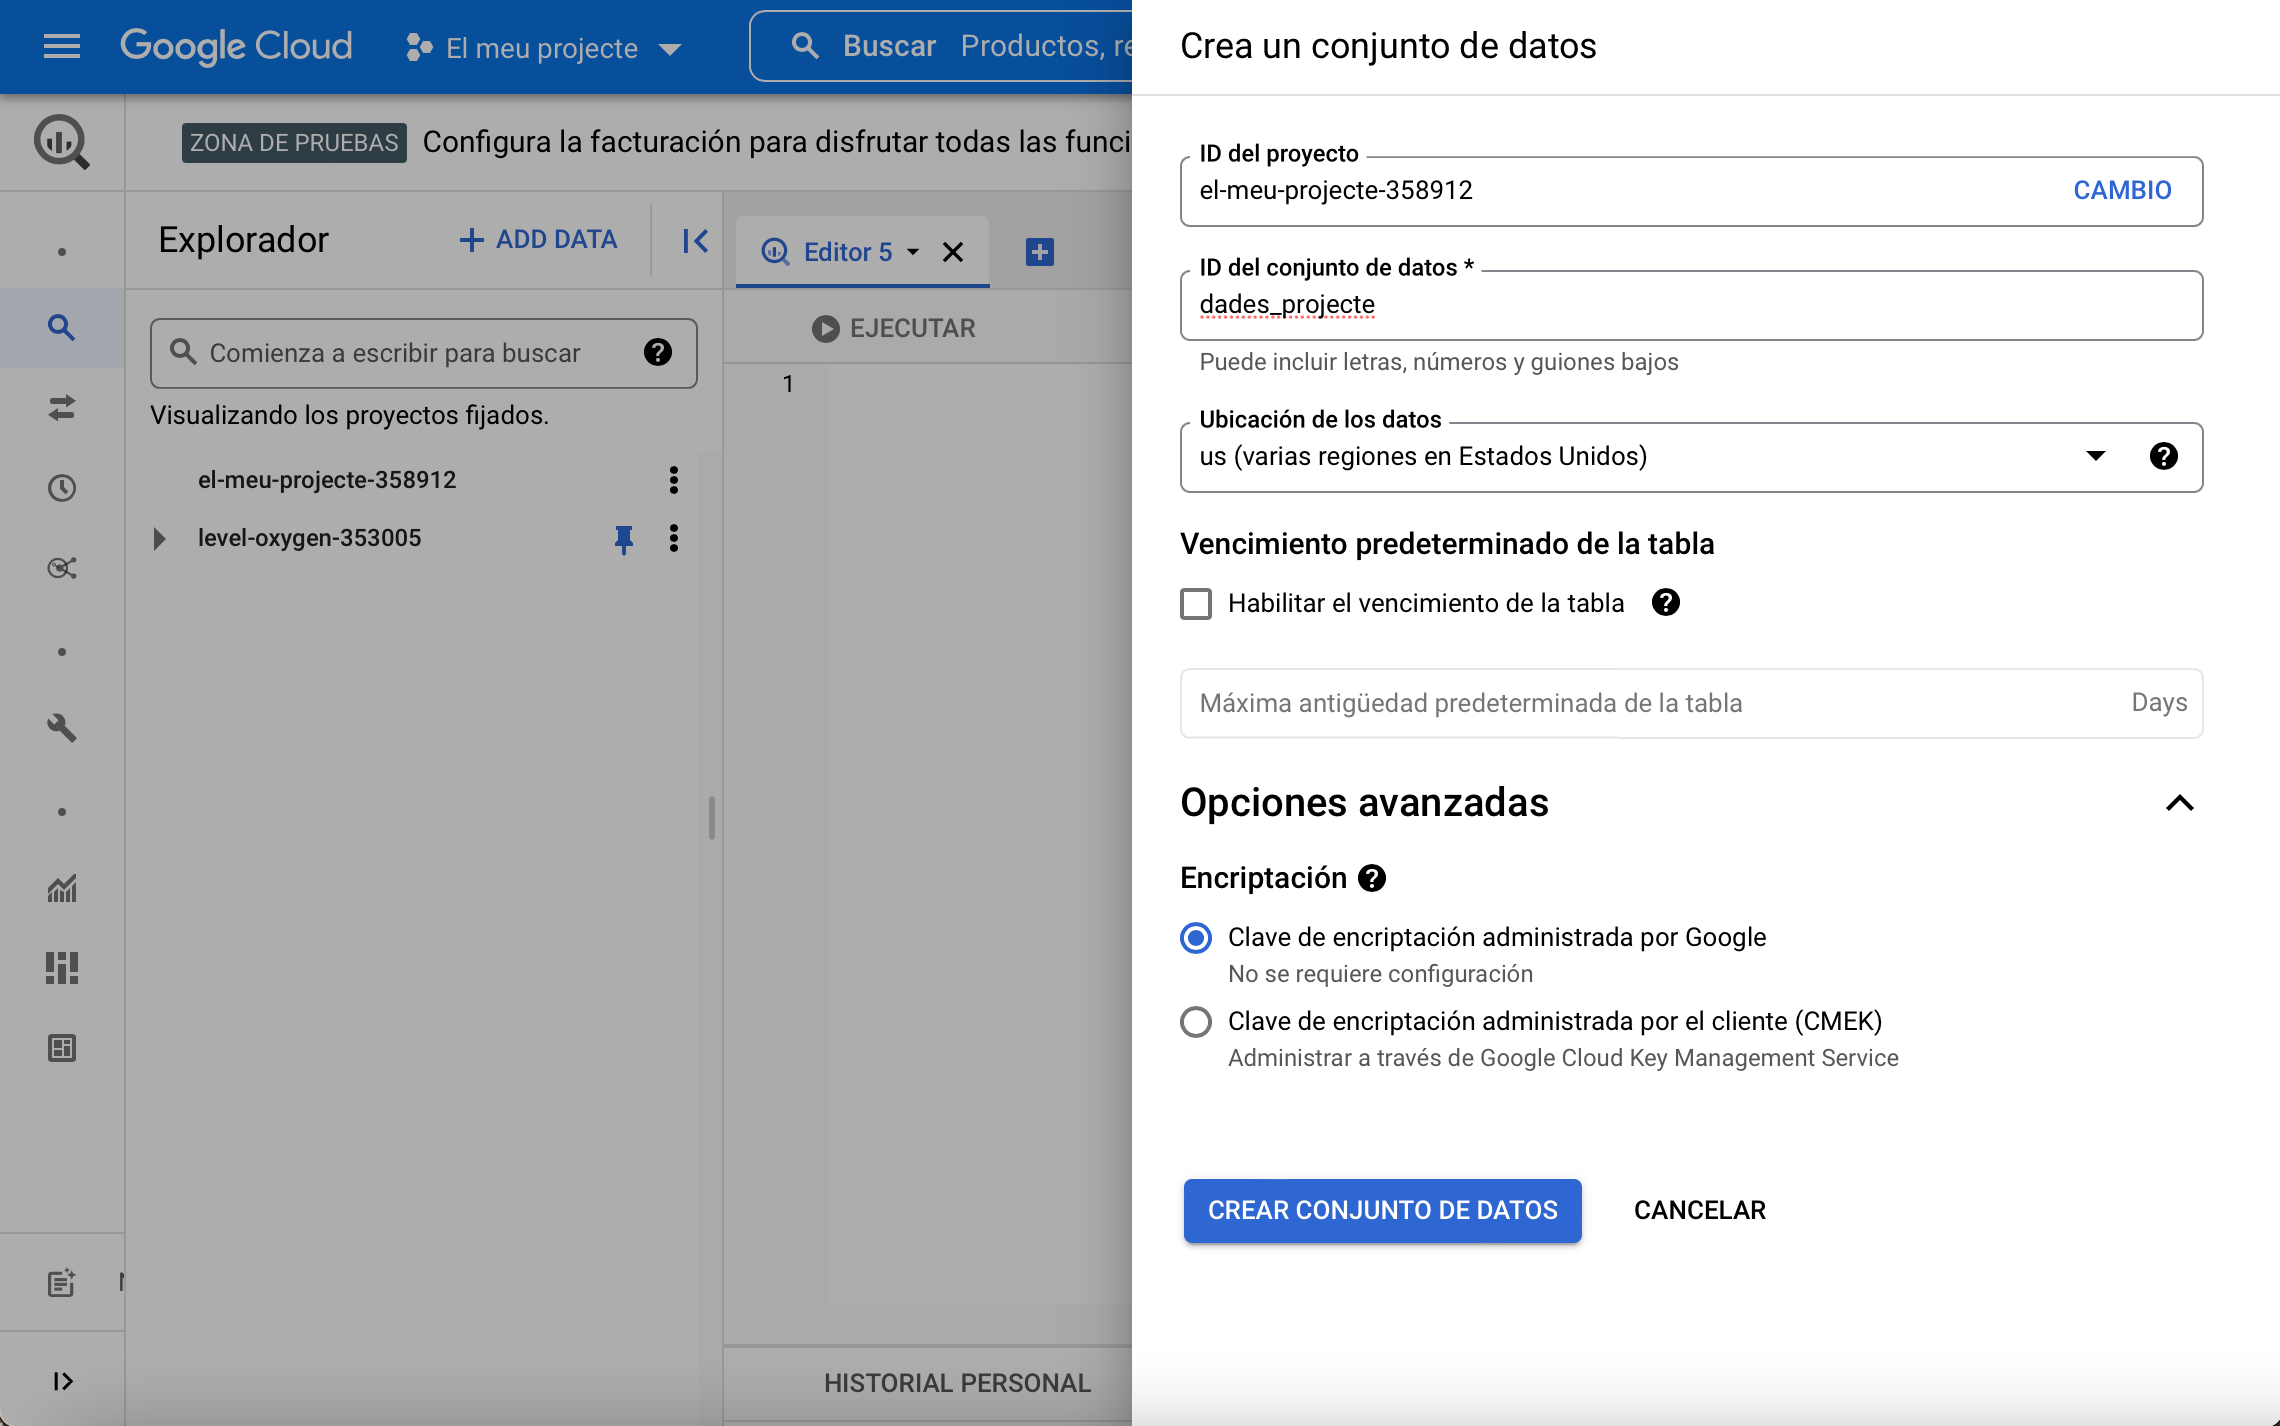
\includegraphics[width=10cm]{bq5}
\end{center}
\caption{Informació del conjunt de dades}
\label{fig:bq5}
\end{figure}
\vspace{2mm}

Un cop creat, el conjunt de dades \verb|dades_projecte|, es pot comprovar que ara apareix dins de \verb|el_meu_projecte| a la UI de BigQuery i, ampliant això, s'observa que no hi ha taules dins d'aquest. Ara, es pot donar un cop d'ull als detalls associats a aquest conjunt de dades (Figura ~\ref{fig:bq5}). Des d'aquest menú, podem triar obrir-lo, moment en el qual la informació del conjunt de dades apareix a la dreta. Aquí podem confirmar l'identificador del conjunt de dades, que també assenyala el projecte en el qual s'ha creat el conjunt de dades, i després altres detalls que inclouen les hores de creació i modificació, així com la ubicació d'aquest.

\vspace{2mm}

A més, des d'aquesta finestra podrem compartir el conjunt de dades amb altres usuaris. Hi ha opcions per a copiar i eliminar aquest conjunt de dades. I després, a l'opció \textit{editar detalles}, podem reconfigurar el temps de caducitat de les taules, establir una descripció o afegir etiquetes. Per exemple, si volem marcar aquest conjunt de dades com a pertanyent a un equip, podem establir una etiqueta amb la clau d'equip i el valor corresponent. En acabant, quan guardem aquest conjunt de dades, les etiquetes apareixen a l'apartat d'informació.

\subsection{Definició d'una taula de BigQuery des de la interfície d'usuari}

Després d'haver creat un conjunt de dades en un projecte, ja es pot crear una taula dins d'aquest conjunt de dades. Si tenim la informació del conjunt de dades, hauríem de veure aquesta opció per a crear una nova taula des d'aquí. Alternativament, podem dirigir-nos al projecte, després al conjunt de dades i triar l'opció de crear una taula. Apareixerà un formulari i tindrem l'opció d'especificar una font per a la nostra taula. Això ens permetrà extreure dades de fonts ja existents, com l'emmagatzematge en el núvol de Google o bé un arxiu dels nostres propis sistemes. La primera taula que crearem serà bastant simple, i ens servirà per explorar una mica la plataforma. De fet, serà una taula buida anomenada \verb|accidents| (Figura ~\ref{fig:bq6}). 

\vspace{2mm}
\begin{figure}[h!]
\par
\raisebox{-.5\height}{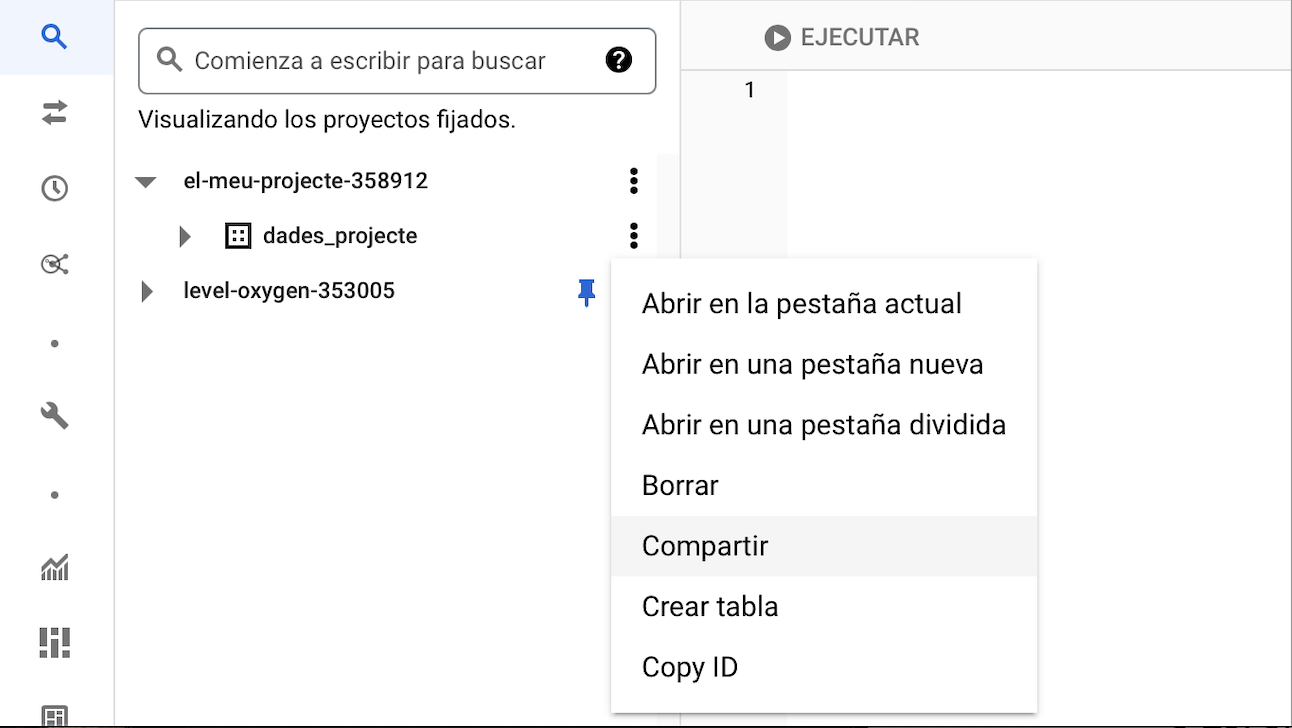
\includegraphics[width=7.25cm]{bq6}}%
\hfill
\raisebox{-.5\height}{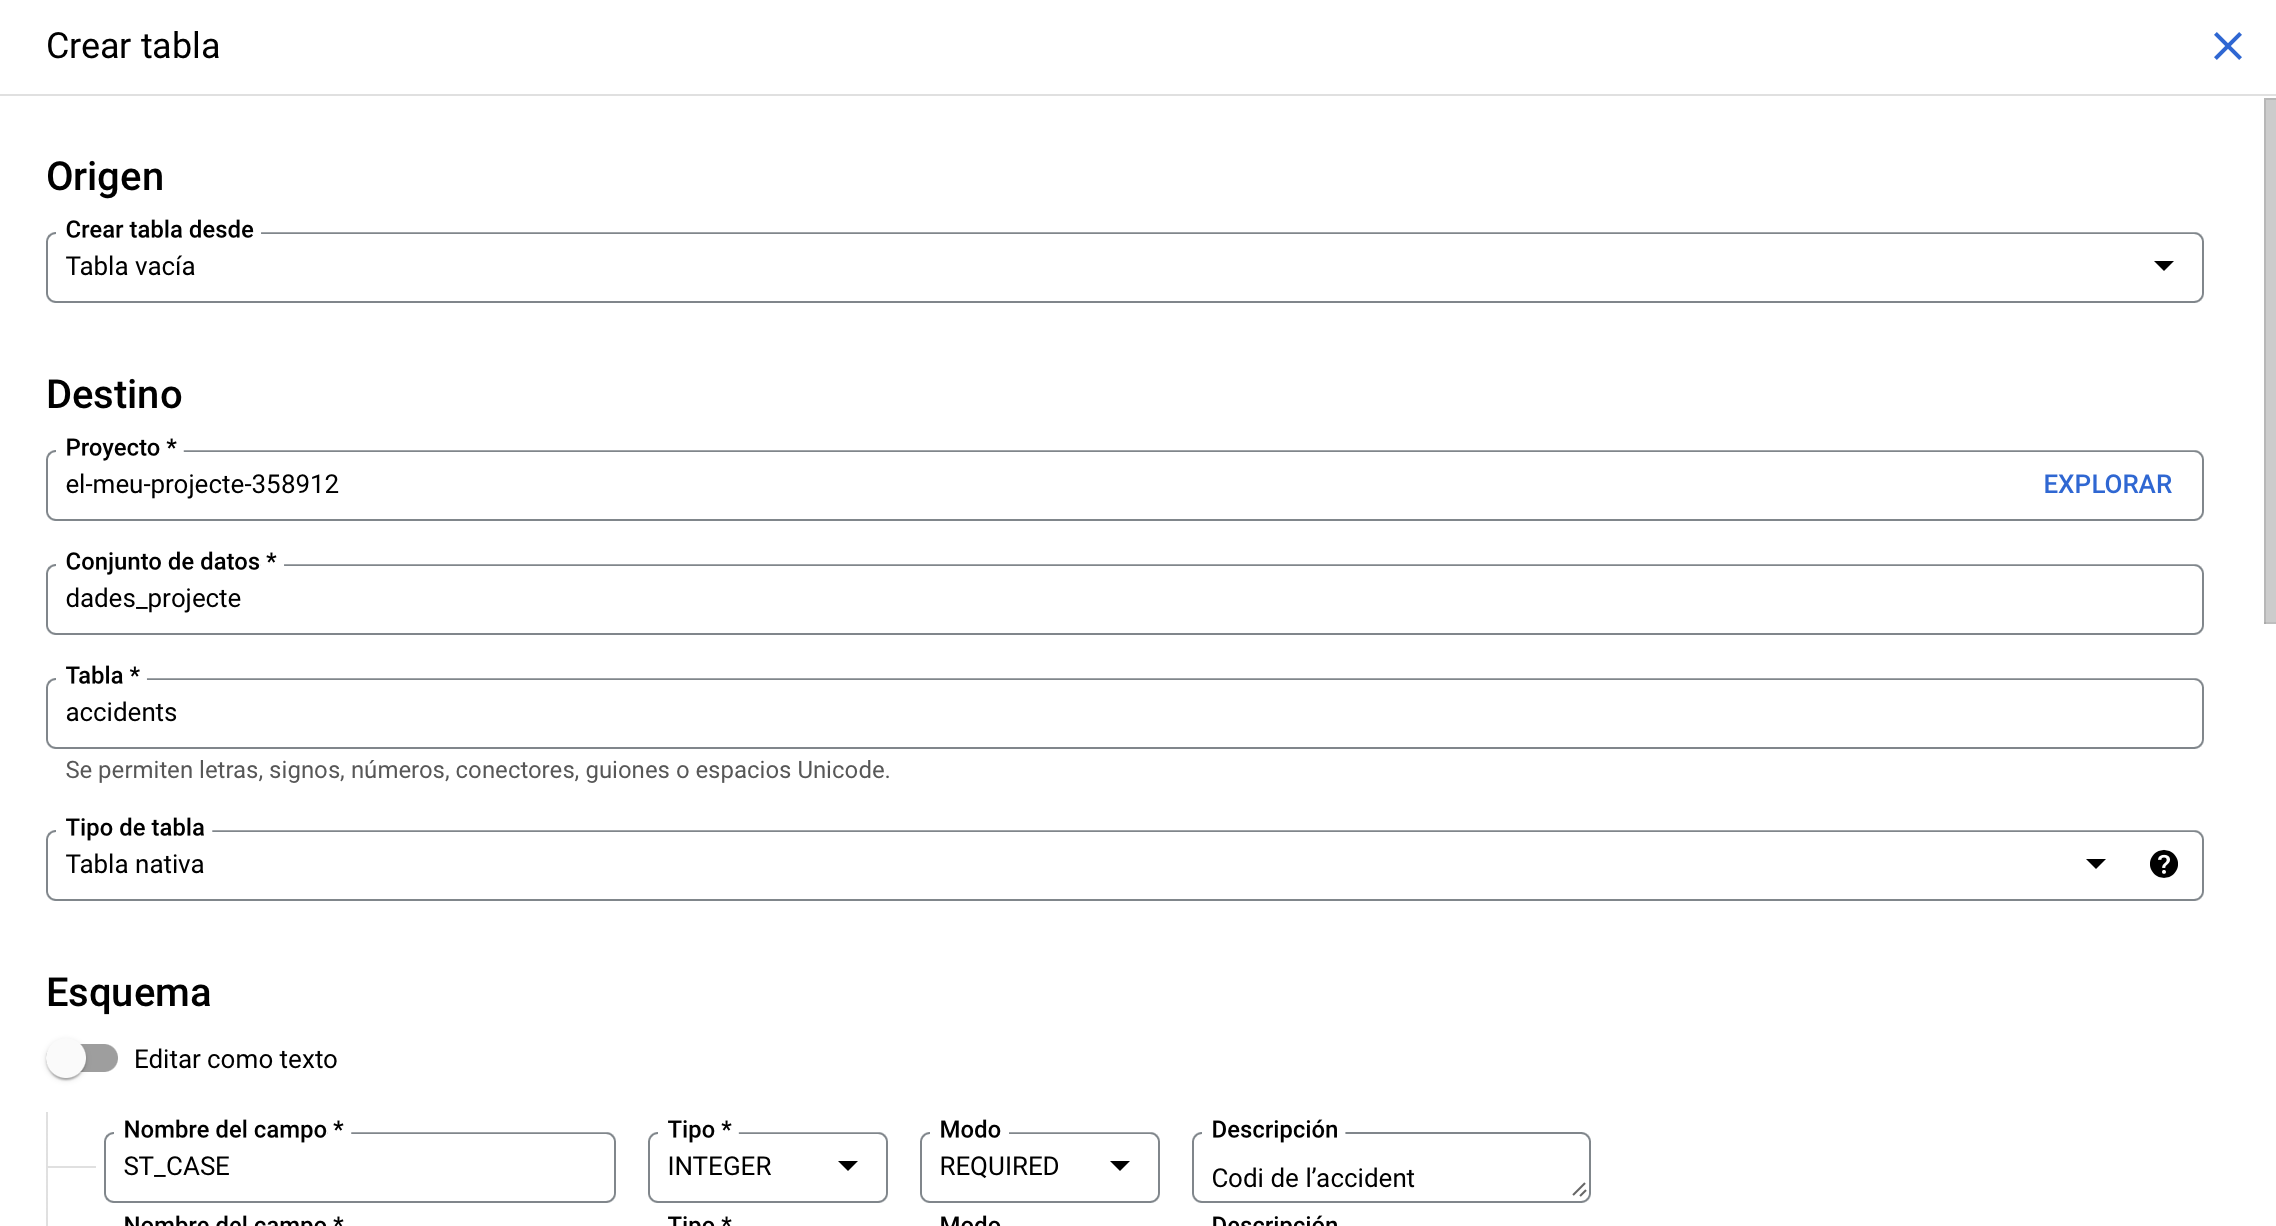
\includegraphics[width=7.25cm]{bq7 copia}}%
\par
\caption{Creació d'una taula}
\label{fig:bq6}
\end{figure}
\vspace{2mm}

A continuació, passem a la secció d'Esquema. Podem fer ús d'aquesta interfície per a establir les columnes de la nostra taula, incloent-hi els tipus i altres configuracions. La primera columna que definiré és l'identificador de l'accident, que s'anomenarà \verb|ST_CASE|. Per al tipus de variable, podem triar d'entre menú d'opcions, que inclou tots els tipus amb els quals ja estem familiaritzats. Quant a la manera (columna \textit{modo} a la figura ~\ref{fig:bq8}), aquesta determinarà si els valors d'aquesta columna poden ser nuls o si es requereix un valor (com és el cas de l'identificador), i també podem establir que els valors siguin d'un tipus que es pugui repetir, marcant \textit{indistint}. Finalment, es pot escriure una descripció per a la variable, que és opcional. 

\vspace{2mm}
\begin{figure}[h!]
\begin{center}
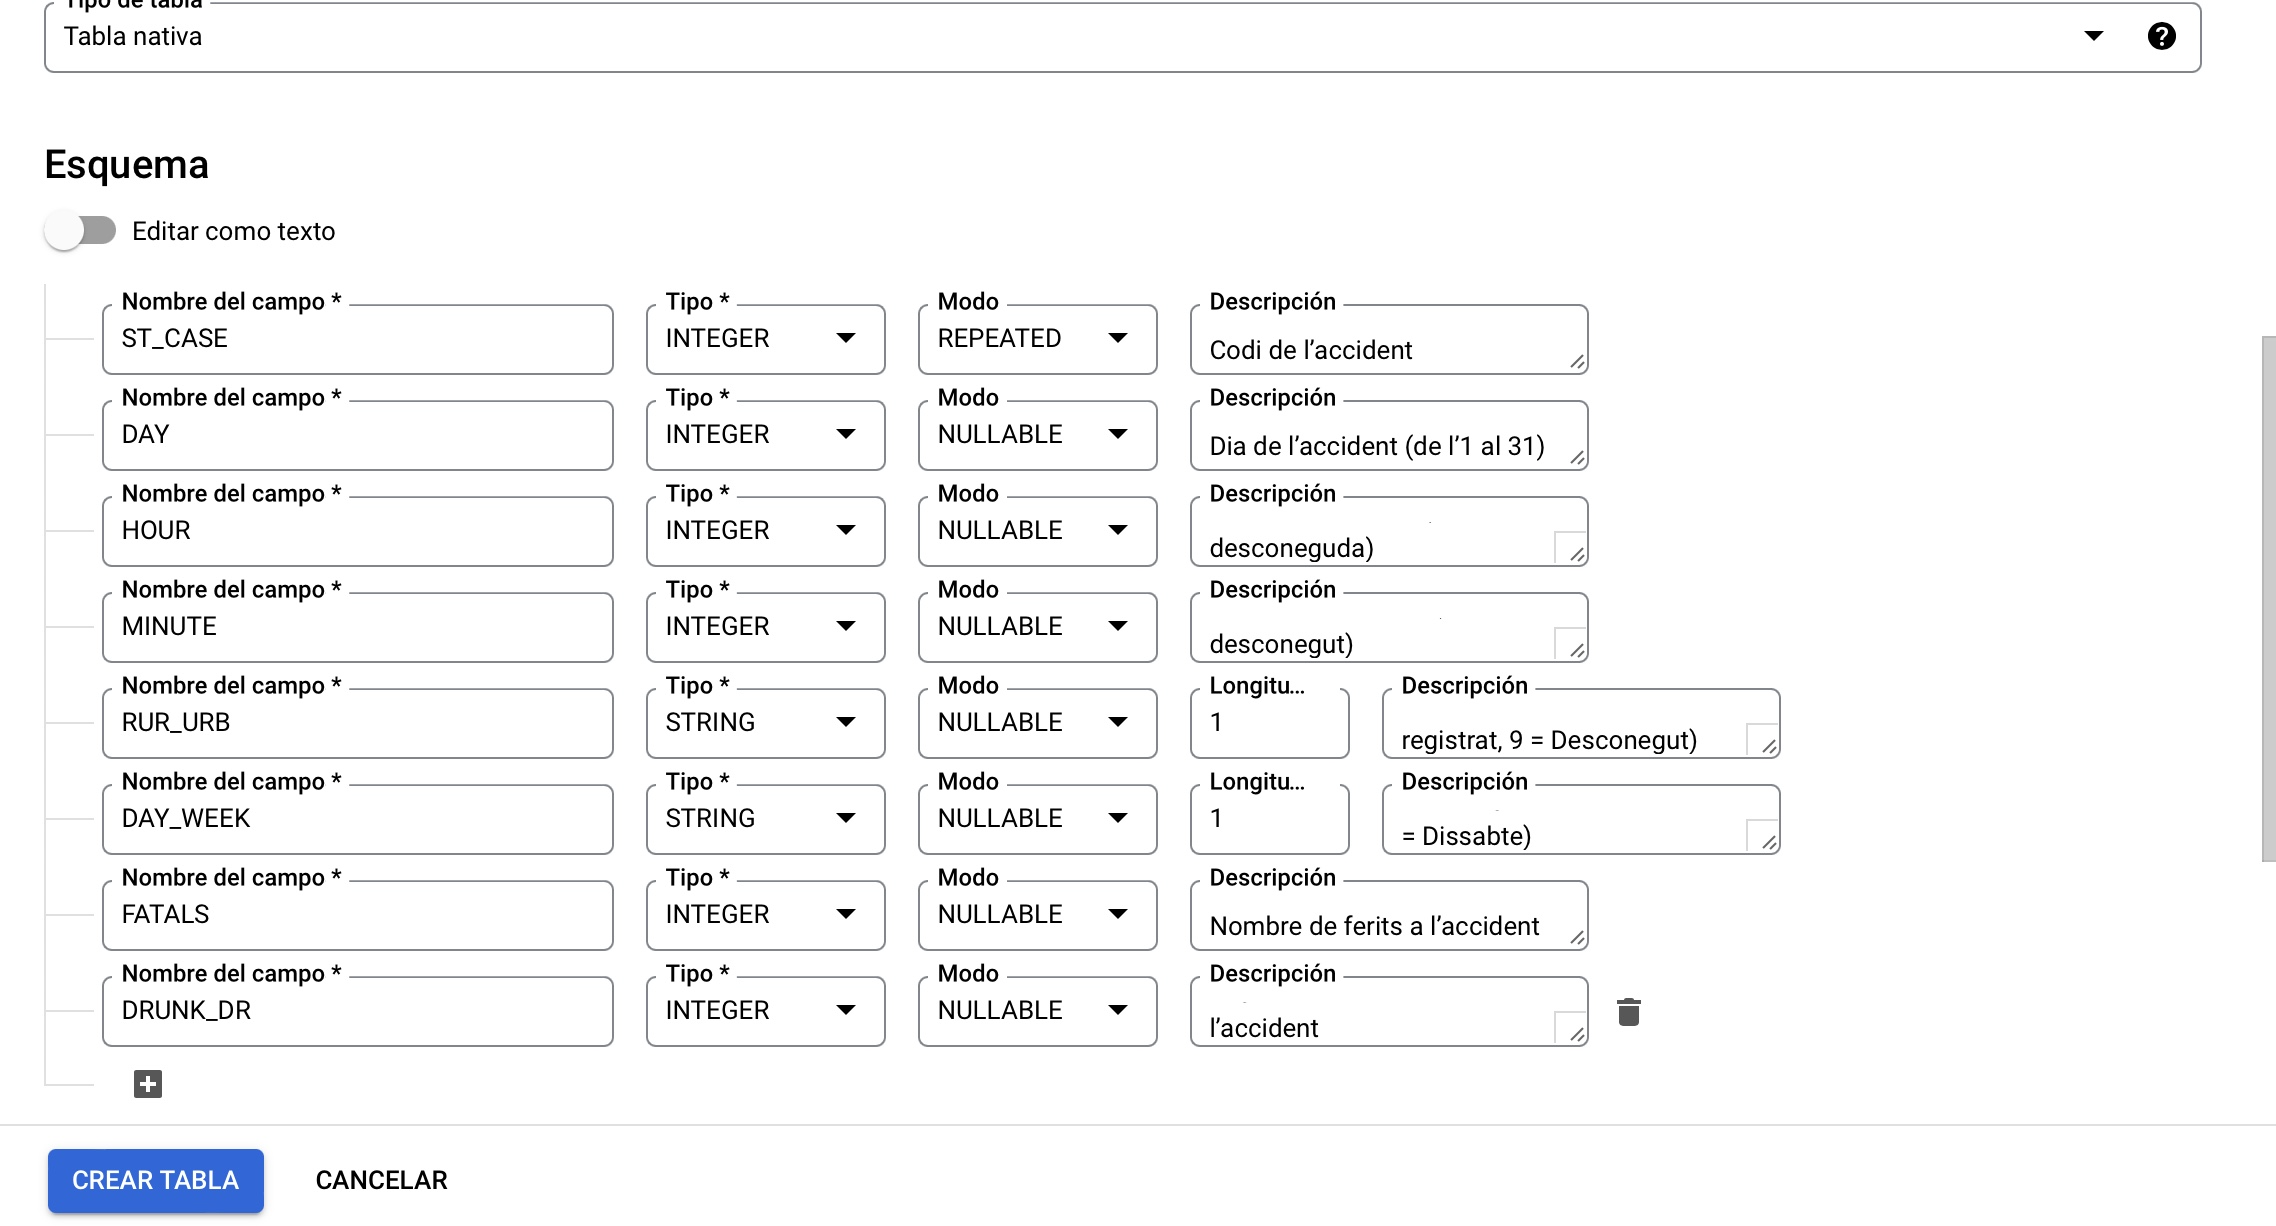
\includegraphics[width=10cm]{bq8}
\end{center}
\caption{Esquema de la nostra taula}
\label{fig:bq8}
\end{figure}
\vspace{2mm}

La taula ~\ref{tab:taula1} que acabem de crear està formada per 8 variables, 6 de les quals són numèriques i 2 categòriques, i es descriuen tal com es pot veure a continuació.

\begin{table}[h]
\resizebox{\textwidth}{!}{%
\begin{tabular}{|l|l|l|}
\hline
Variable  & Tipus      & Descripció                                                                                                        \\ \hline
ST\_CASE       & Numèrica & Codi de l'accident                                                                                   \\ \hline
DAY       & Numèrica & Dia de l’accident (de l’1 al 31)                                                                                    \\ \hline
HOUR      & Numèrica   & Hora de l’accident (99 = desconeguda)                                                                               \\ \hline
MINUTE    & Numèrica   & Minut de l’accident (99 = desconegut)                                                                               \\ \hline
RUR\_URB  & Categòrica & Informació sobre la localització (1 = Rural, 2 = Urbà, 6 = Via no classificada, 8 = No registrat, 9 = Desconegut)   \\ \hline
DAY\_WEEK & Categòrica & Dia de la setmana (1 = Diumenge, 2 = Dilluns, ..., 7 = Dissabte)                                                    \\ \hline
FATALS    & Numèrica   & Nombre de ferits a l’accident                                                                                       \\ \hline
DRUNK\_DR & Numèrica   & Nombre de conductors beguts involucrats a l’accident                                                                \\ \hline
\end{tabular}%
}
\caption{Especificacions de la taula Accidents}
\label{tab:taula1}
\end{table}

\vspace{2mm}

En el transcurs del treball, farem ús d'aquesta taula, juntament amb dues més, que prenen de nom de \verb|persones| i \verb|vehicles|, per analitzar les dades que es van prendre d'un conjunt d'accidents que es van donar als Estats Units. 

\subsubsection{Afegir dades a una taula de BigQuery senzilla}

Ara que hem creat una taula de consulta, podem centrar-nos a treballar amb ella. Per a això, ens desplaçarem cap avall i donarem un cop d'ull al primer esquema de la taula (a la figura ~\ref{fig:bq9}), on es troba a alguna informació interessant. Més enllà de la identificació de la taula, a l'esquerra de la figura, també podem comprovar la grandària de la taula a la dreta, que ens donarà una indicació de la quantitat de dades que es processaran, si anéssim a executar consultes sobre aquesta. La grandària d'emmagatzematge a llarg termini assenyala les dades a les quals no s'ha accedit en els últims noranta dies, i després, per descomptat, tenim les hores de creació i modificació juntament amb la ubicació de les dades de la taula. Des d'aquesta interfície, també podem editar els detalls existents d'aquesta taula. Aquí podem establir un temps de caducitat en cas que vulguem anul·lar el que s'ha establert en el nivell del conjunt de dades. També tenim l'opció d'establir una descripció o afegir etiquetes.

\vspace{2mm}
\begin{figure}[h!]
\par
\raisebox{-.5\height}{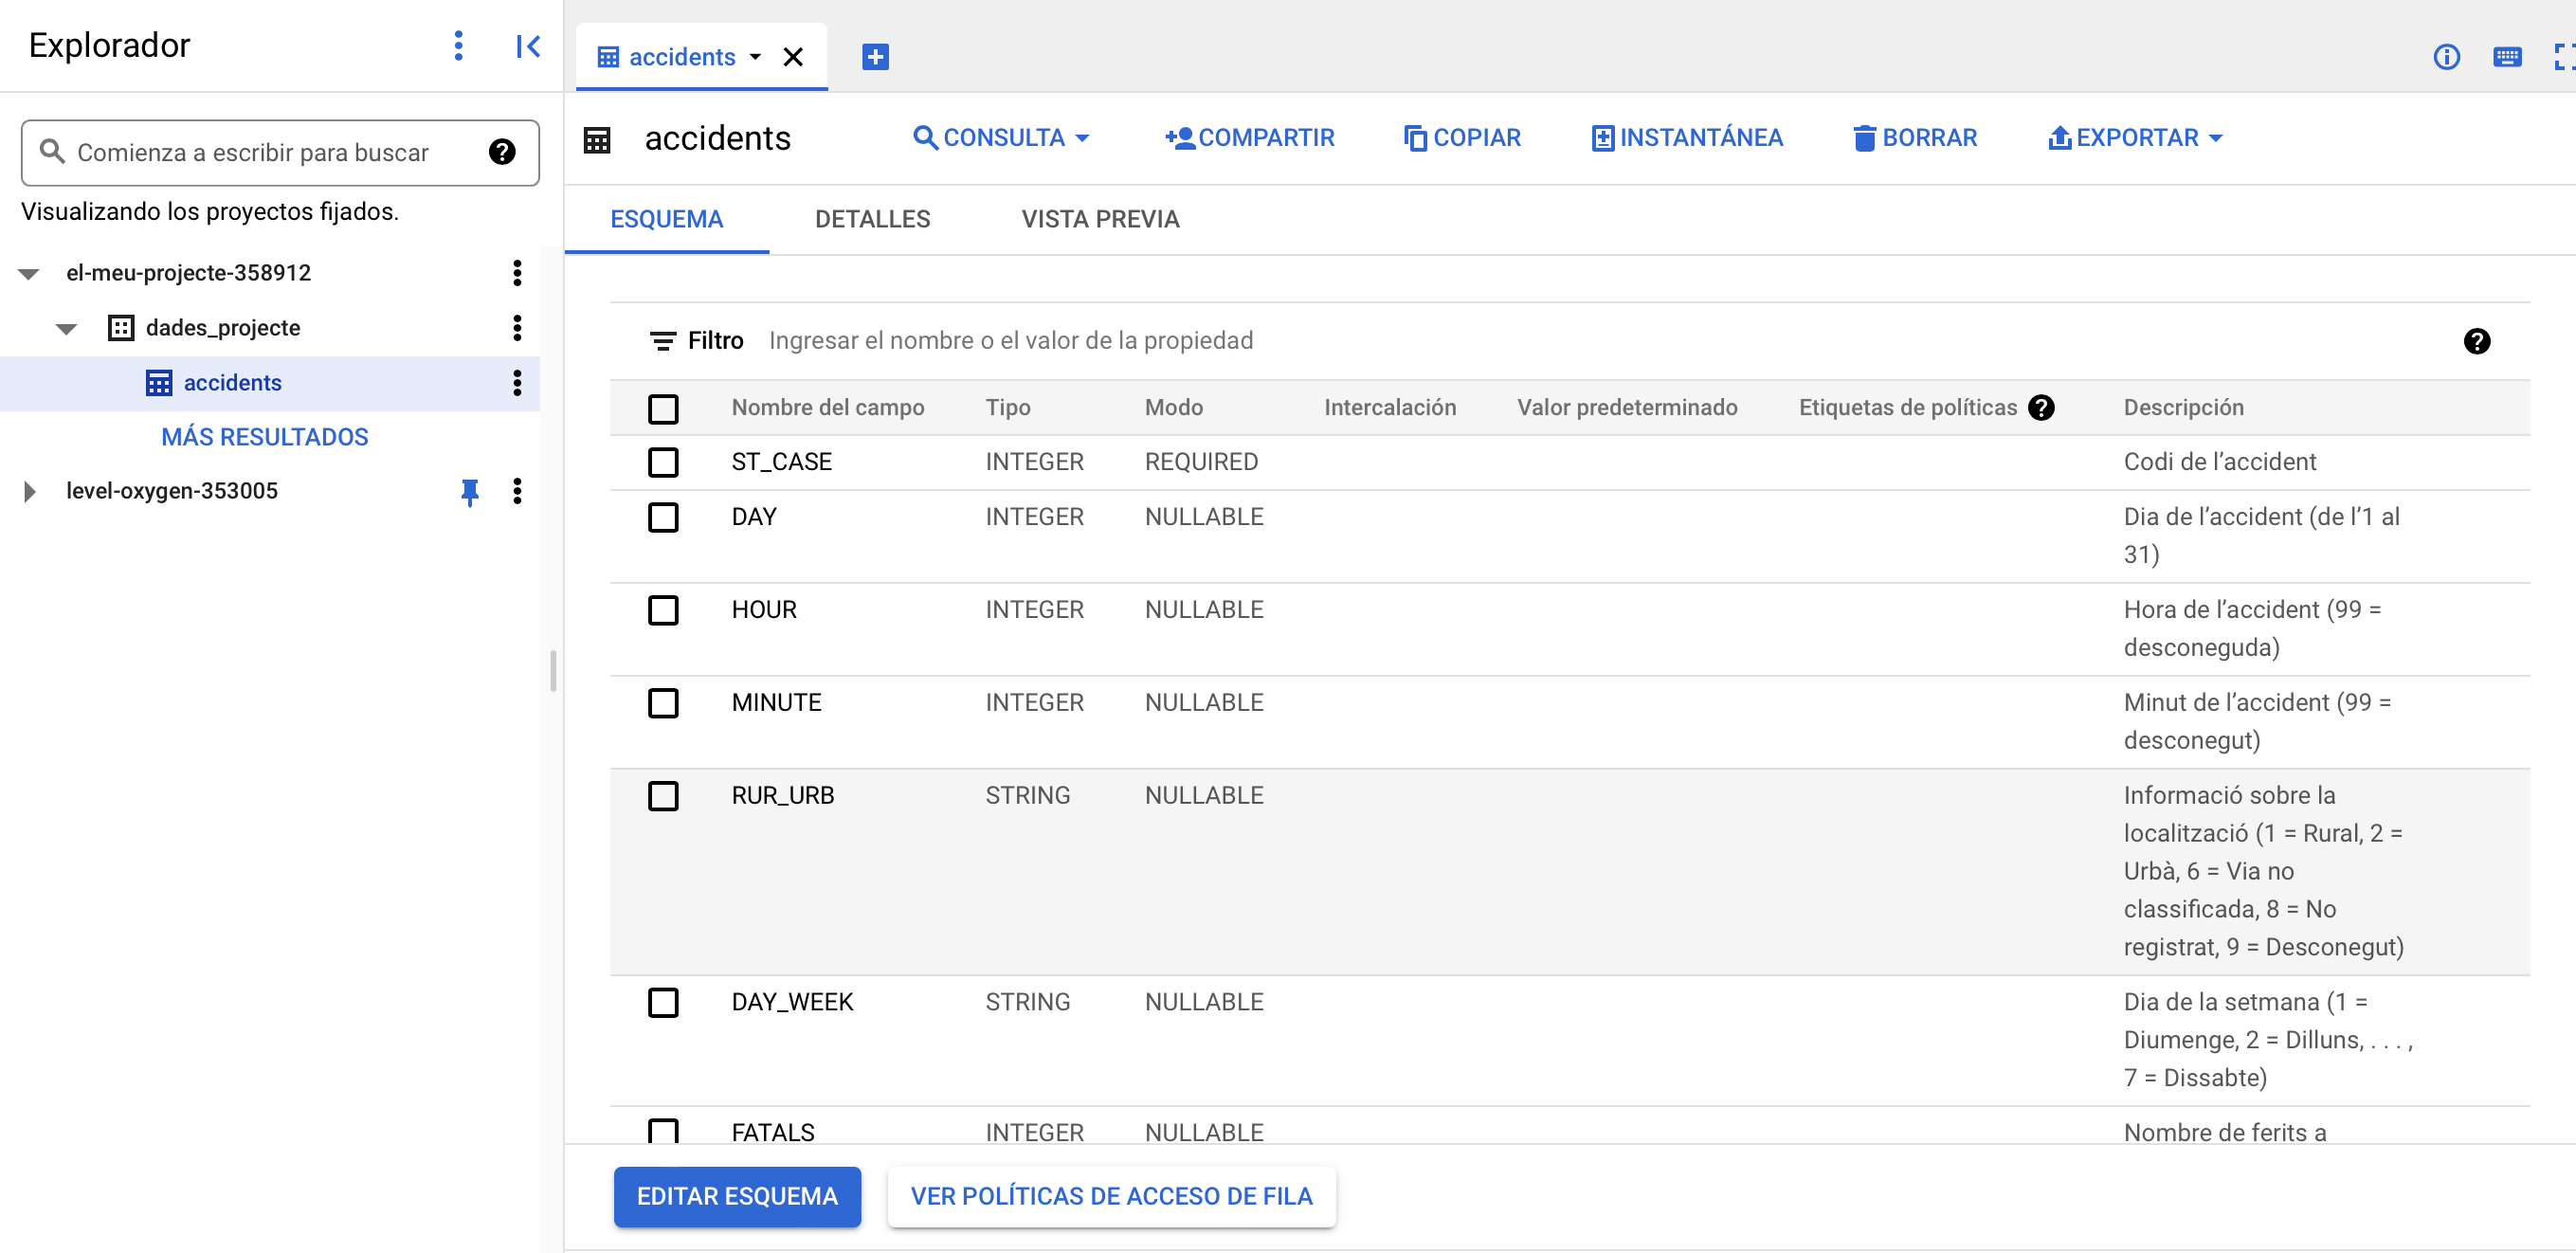
\includegraphics[width=7.25cm]{bq9}}%
\hfill
\raisebox{-.5\height}{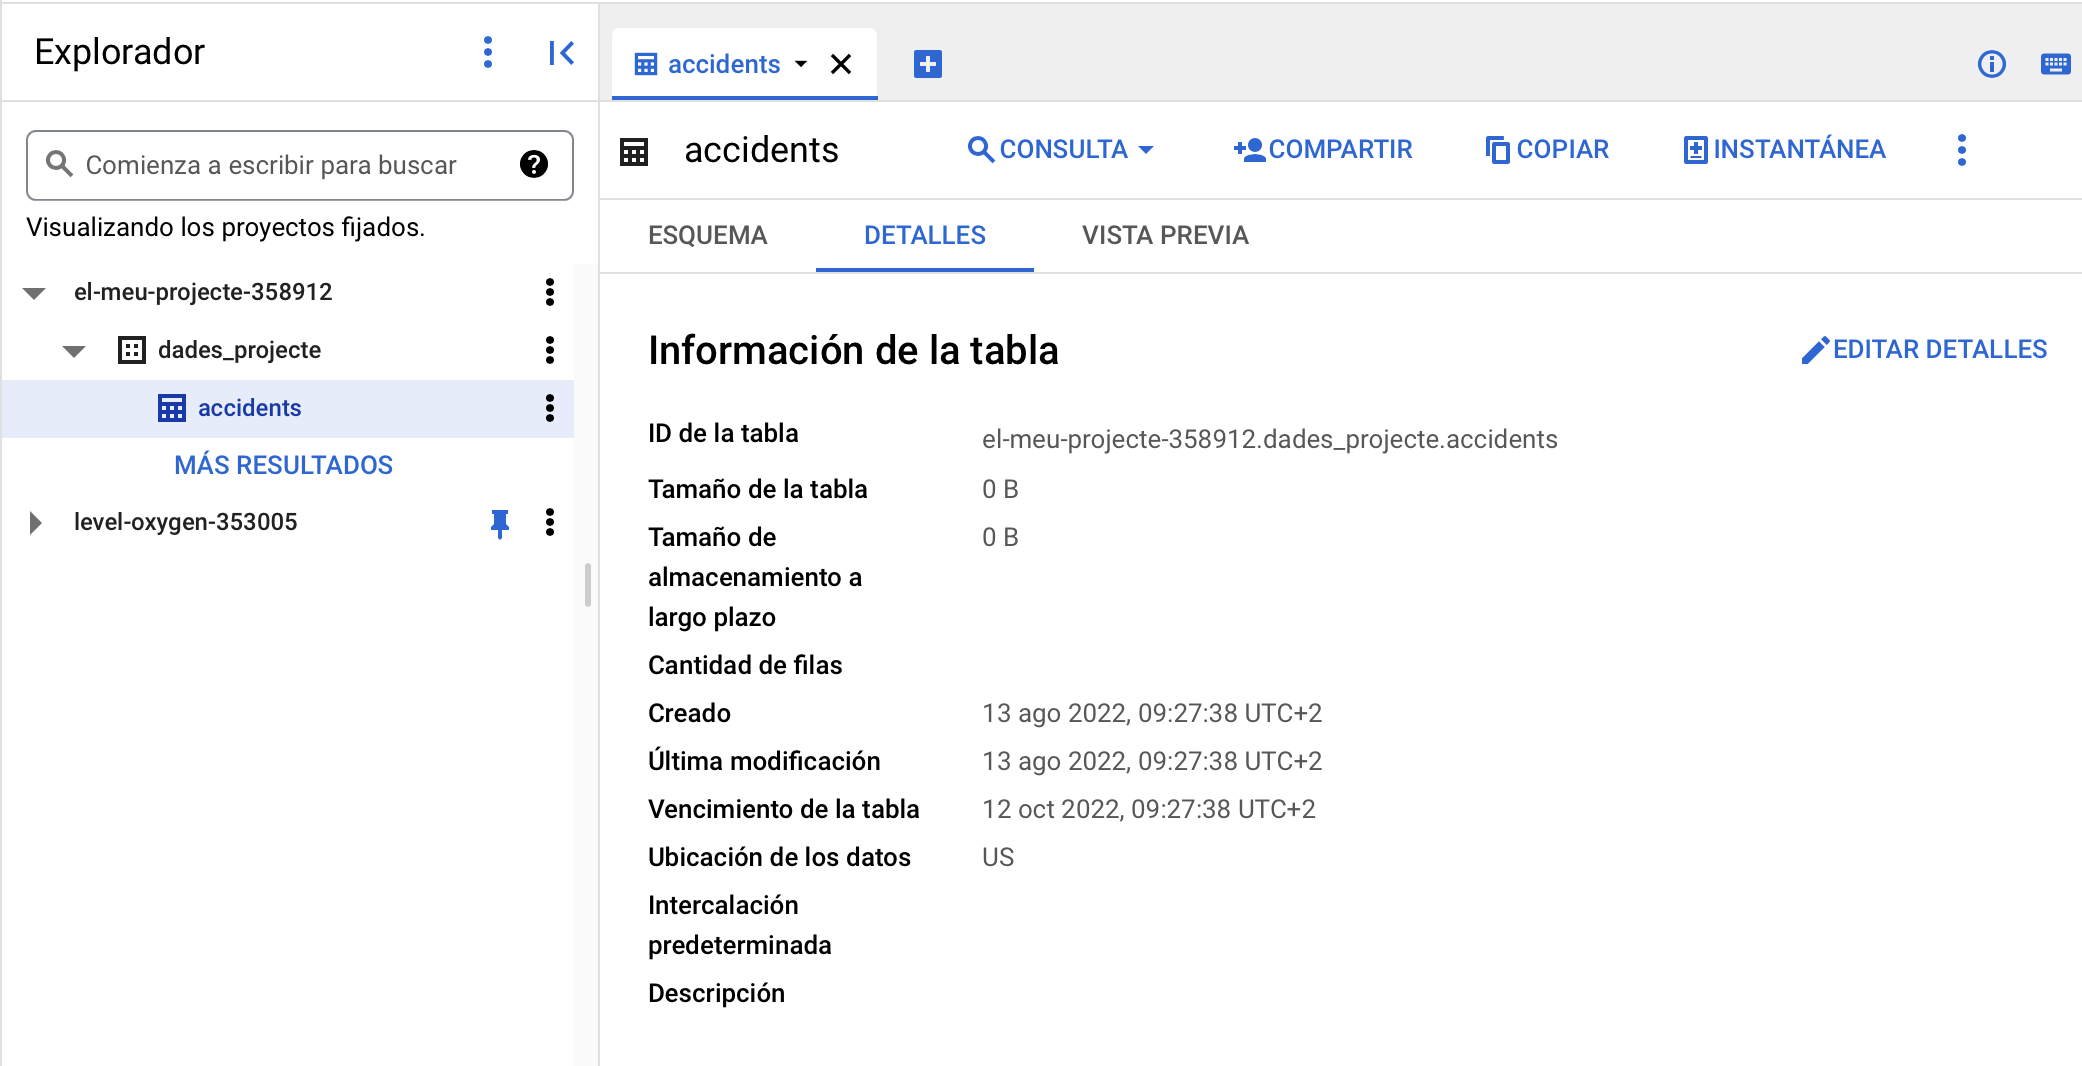
\includegraphics[width=7.25cm]{bq10}}%
\par

\caption{Detalls de la taula}
\label{fig:bq9}
\end{figure}
\vspace{2mm}

Una altra característica que podem consultar és la vista prèvia de la taula, i com és lògic, veurem que aquesta encara no conté dades, ja que simplement hem creat l'esquema de la taula, sense inserir cap dada en aquesta. Si féssim ús de SQL, en qualsevol altre context es podrien afegir dades a partir d'una simple consulta a la taula, que tindria l'estructura següent:

\begin{verbatim}
INSERT INTO `el-meu-projecte-358912.dades_projecte.accidents` 
(ST_CASE, DAY, HOUR, MINUTE, RUR_URB, DAY_WEEK, FATALS, DRUNK_DR)
VALUES (20055, 1, 20, 55, "1", "3", 3, 0);
\end{verbatim}

A partir d'aquesta consulta afegiríem a la taula el cas d'un accident amb identificador 20055, que es va produir el dia 1 del mes a les 20:55 a una zona rural (\verb|RUR_URB| = 1)un dimarts (\verb|DAY_WEEK| = 3), i en el que hi ha 3 ferits i cap conductor begut involucrat en l'accident.

Això no obstant, quan intentem executar la consulta, BigQuery ens informa d'un error (Figura ~\ref{fig:bq11}). Si recordem, prèviament s'han definit algunes de les limitacions per a l'ús de la zona de proves de BigQuery. Entre aquestes s´hi troba que no podem utilitzar el llenguatge de manipulació de dades (DML), és a dir, que no podem modificar la taula amb sentències com \verb|INSERT INTO|, \verb|UPDATE| o \verb|DELETE|, per exemple. Per aquest motiu, l'error ens avisa que no tenim el nostre projecte vinculat a un compte i, per tant, no ens avaluarà la nostra consulta.

\vspace{2mm}
\begin{figure}[h!]
\begin{center}
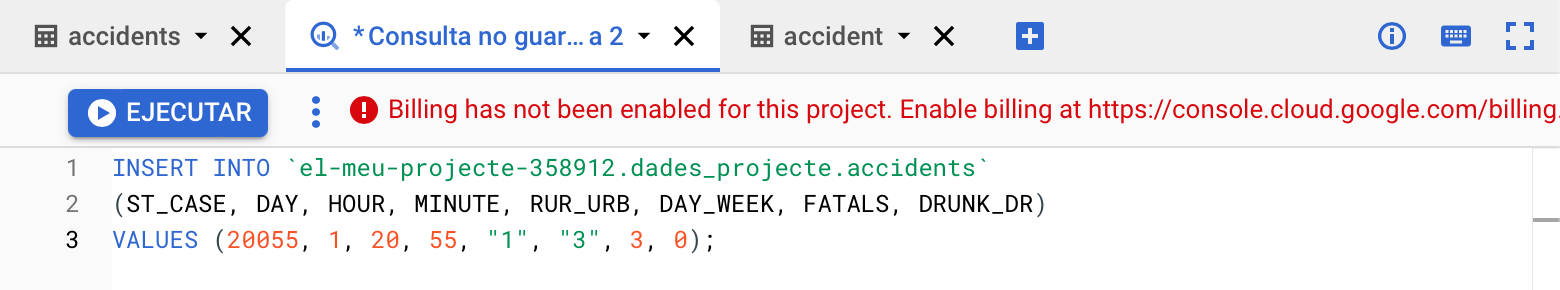
\includegraphics[width=12cm]{bq11}
\end{center}
\caption{Inserció de dades a la taula}
\label{fig:bq11}
\end{figure}
\vspace{2mm}

\subsection{Càrrega de dades per crear una taula de BigQuery}

Hem vist que és possible crear una taula buida, però que la zona de proves (\textit{sandbox}) no ens permet després emplenar-la amb dades amb sentències \verb|INSERT|. Ara explorarem un cas d'ús més comú per als usuaris de BigQuery en el qual es crea una taula a partir de dades existents. Per a això, ens dirigirem al nostre conjunt de dades, \verb|dades_projecte|, i triarem crear una nova taula. Aquest cop, la font no serà una taula buida, sinó que carregarem un arxiu CSV del nostre propi sistema d'arxius. Un cop seleccionem importar les dades, es pot seleccionar diferents tipus d'arxiu com ara CSV, JSON, Avro o Parquet, principalment. Per a respectar les limitacions de la zona de proves, hi ha algunes restriccions quant a la grandària de l'arxiu que podem pujar, recordem que aquestes han de ser menors a 10 Gb. Procedim llavors a navegar pels nostres sistemes d'arxius per a l'arxiu a pujar. Una vegada que l'arxiu ha estat seleccionat, el format de l'arxiu s'ha establert automàticament en CSV (Figura ~\ref{fig:bq12}). 

\vspace{2mm}
\begin{figure}[h!]
\par
\raisebox{-.5\height}{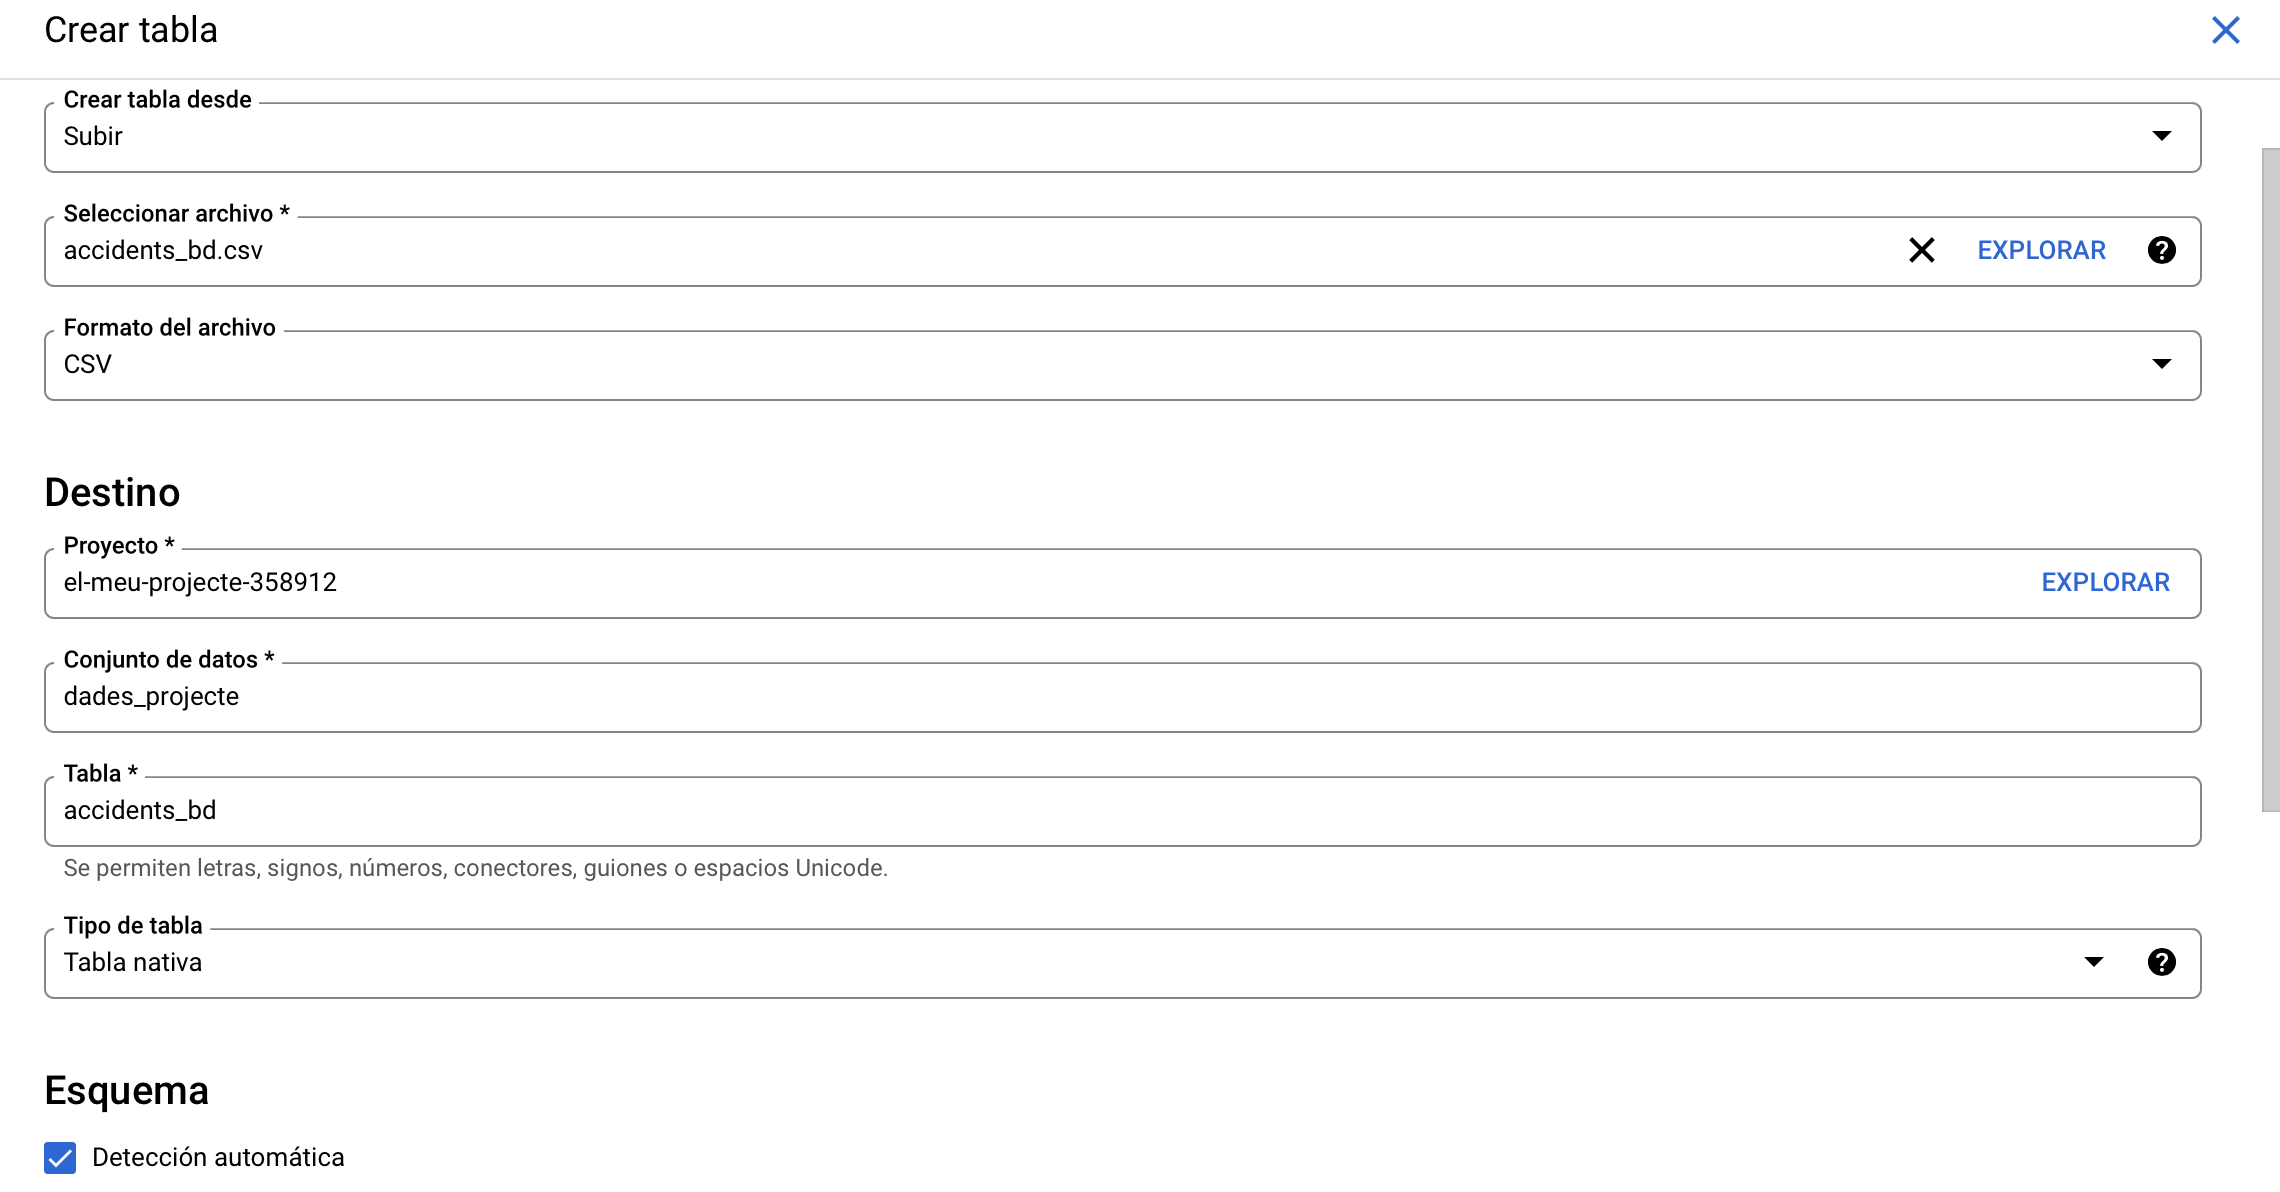
\includegraphics[width=7.25cm]{bq12}}%
\hfill
\raisebox{-.5\height}{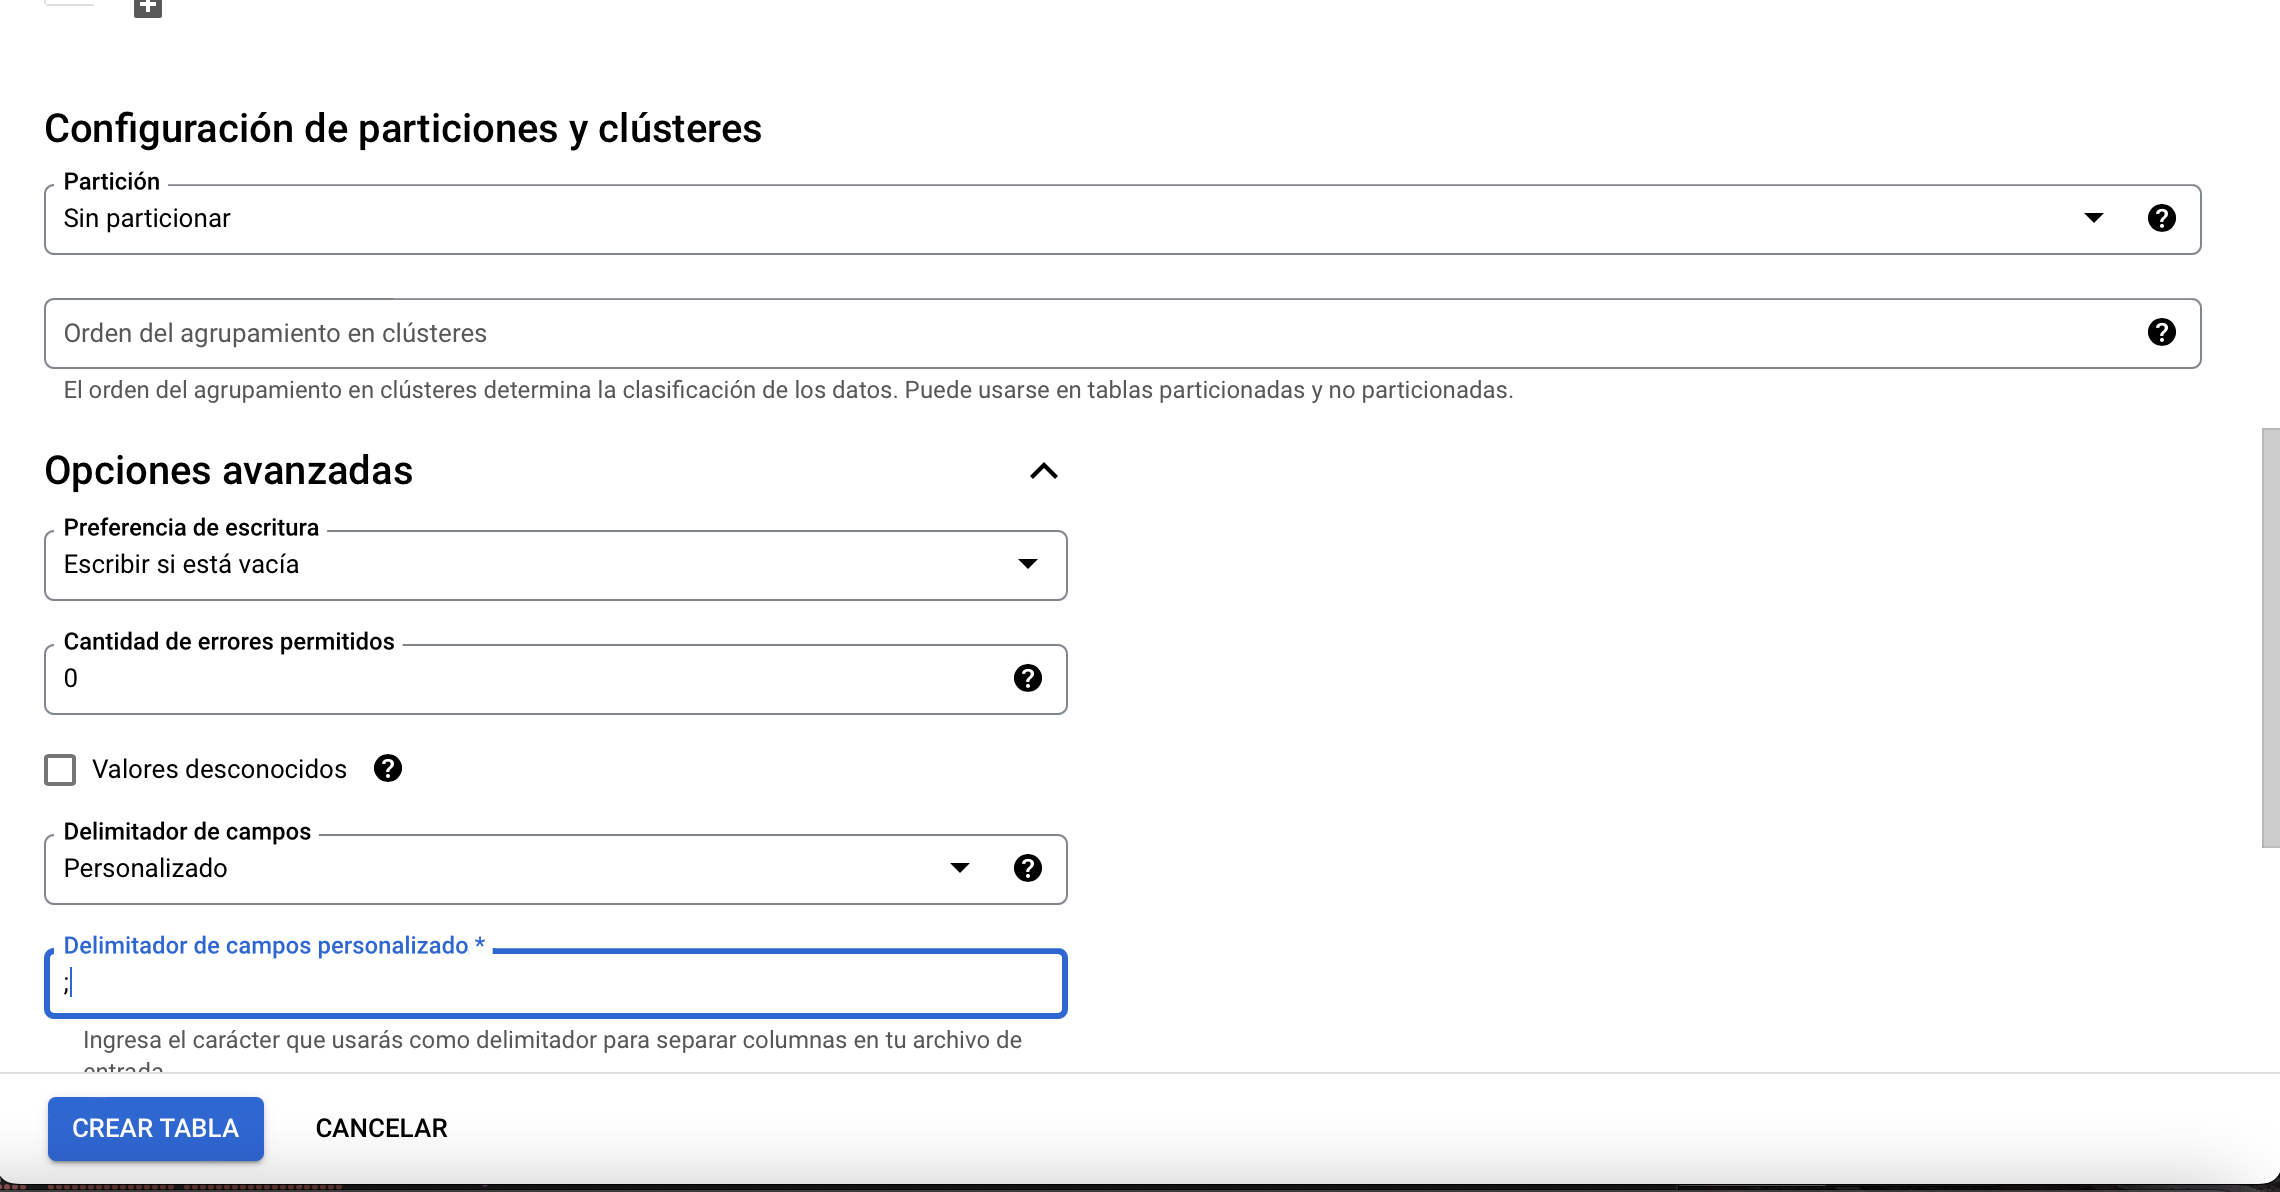
\includegraphics[width=7.25cm]{bq13}}%
\par

\caption{Lectura d'un arxiu extern}
\label{fig:bq12}
\end{figure}
\vspace{2mm}

Quant al projecte i al conjunt de dades, els deixarem com estan. I escollirem el nom de la taula, \verb|accidents_bd|, el qual farà saber que inclou informació sobre diversos accidents de trànsit. A continuació, tenim l'opció de definir explícitament l'esquema. No obstant això, atès que es tracta d'un arxiu CSV amb múltiples columnes, podem triar l'opció de detectar automàticament. D'aquesta manera, BigQuery donarà un cop d'ull al contingut de cada columna i determinarà quin ha de ser l'esquema. Més enllà d'això, al final de la finestra de creació de la taula ens apareixeran unes Opcions avançades. Aquestes opcions permeten la lectura de diferents tipus de CSV, entre altres coses. Sabem que el delimitador de camps d’un CSV pot ser una tabulació o una coma entre altres possibilitats. En el nostre cas, cal especificar que el nostre tabulador és el punt i coma “;”. 

\vspace{2mm}

Si hem establert totes aquestes especificacions, ja podrem començar amb l’anàlisi.

\vspace{2mm}

Ara es pot comprovar que \verb|accidents_bd| apareix sota el nostre conjunt de dades, \verb|dades_projecte|. A continuació, podem accedir a la informació de la taula i al seu contingut desplegant el menú i triant Obrir. En l'esquema de la taula, sabrà que s'ha detectat automàticament el tipus dels diferents camps. Donem un cop d'ull als detalls de la taula. Aquí notaràs que la grandària total és de poc més de 280 kB. El nombre de files és d'unes 2.780. I després, quan ens dirigim a la Vista Prèvia, obtenim un cop d'ull als continguts (Figura ~\ref{fig:bq13}). 

\vspace{2mm}
\begin{figure}[h!]
\par
\raisebox{-.5\height}{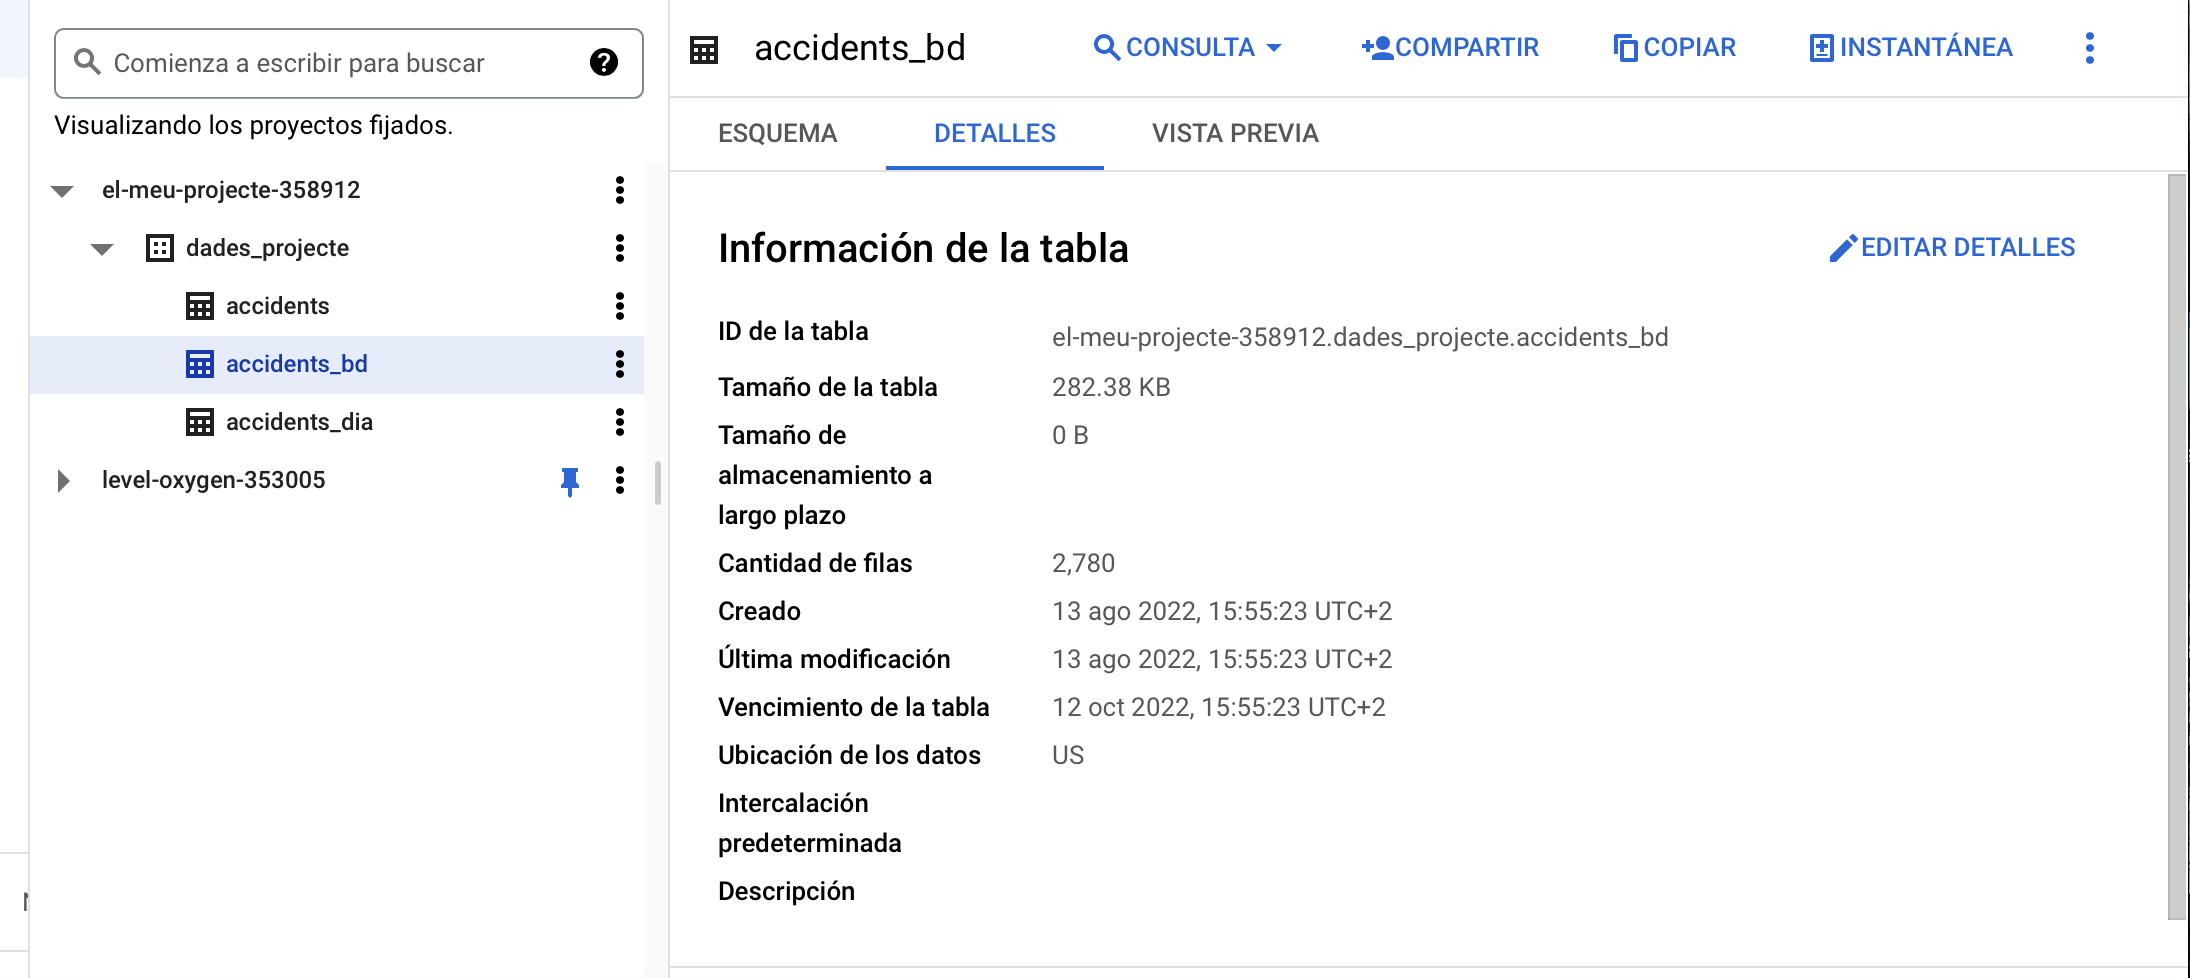
\includegraphics[width=7.25cm]{bq13_2}}%
\hfill
\raisebox{-.5\height}{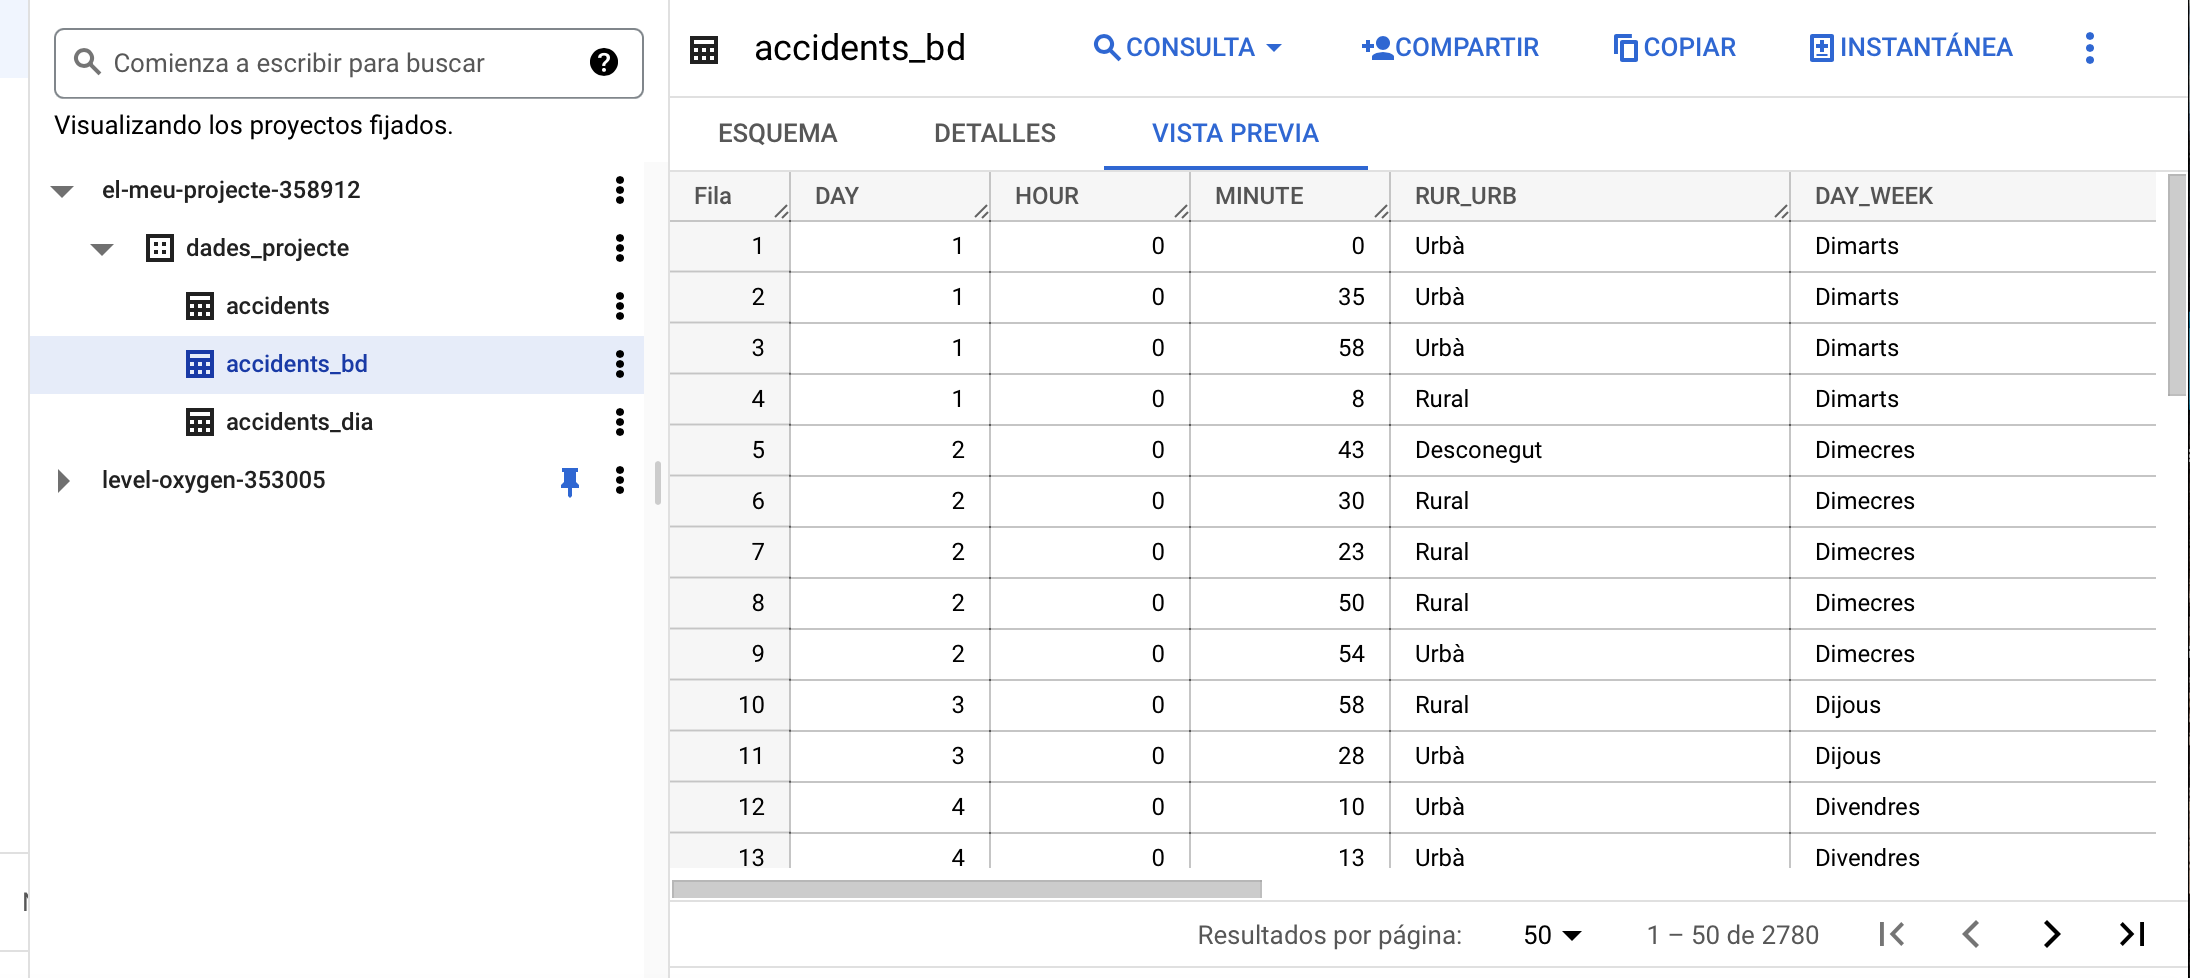
\includegraphics[width=7.25cm]{bq13_3}}%
\par

\caption{Informació sobre la taula}
\label{fig:bq13}
\end{figure}
\vspace{2mm}


\subsection{Consulta de dades i visualització d'estadístiques de consultes}

Per a executar consultes en aquesta taula, ens dirigim al botó de consulta i s'obrirà en una nova pestanya. Aquesta pot ser una pestanya completament nova que ocultarà aquesta vista de detalls, mentre que una pestanya dividida ens permetrà fer referència a aquesta vista de detalls per a la taula mentre construïm una consulta. Mitjançant aquest procés, ha aparegut una nova pestanya cap a la dreta, i la consulta que apareix per defecte inclou una clàusula \verb|SELECT|, però no inclou cap camp (Figura ~\ref{fig:bq14}). Precisament per això hi ha un error de sintaxi, com es mostra a la dreta de la figura. 

\vspace{2mm}
\begin{figure}[h!]
\par
\raisebox{-.5\height}{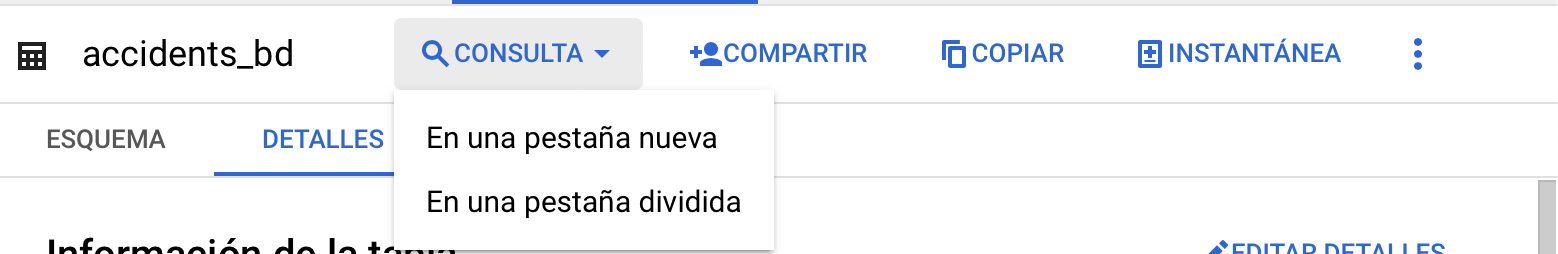
\includegraphics[width=7.25cm]{bq14}}%
\hfill
\raisebox{-.5\height}{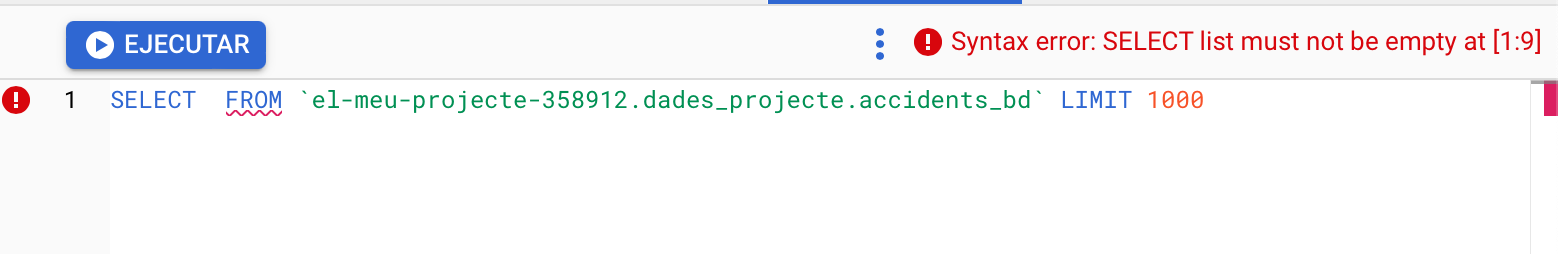
\includegraphics[width=7.25cm]{bq15}}%
\par

\caption{Elaboració d'una consulta}
\label{fig:bq14}
\end{figure}
\vspace{2mm}

Ara, per a completar la clàusula \verb|SELECT|, podríem escriure els noms dels atributs que volem consultar, a més de condicions, per exemple, mitjançant la clàusula \verb|WHERE|. Concretament, l'esquema que s'haurà de seguir per a consultar la base de dades té la forma següent:


\begin{verbatim}
SELECT atribut1, atribut2,...
FROM `[nom_projecte].[nom_base_de_dades].[nom_taula]`
(WHERE condició)
\end{verbatim}

\vspace{2mm}

Si escrivim a l’editor la nostra consulta, apareixerà un validador d’aquesta a la part superior dreta de la finestra. Aquest validador l'hem vist anteriorment quan ens indicava un error en voler executar una consulta fent servir llenguatge de manipulació de dades (DML), i pot agafar dues formes:
- Si la consulta és vàlida, apareixerà una icona de verificación verd.
- Si la consulta no és vàlida, apareixerà una icona d’exclamació Vermell
A més, el validador també mostra la quantitat de dades que la consulta processarà quan s’executi. Per exemple, si demanem en una consulta que ens retorni la columna sencera \verb|DAY|, el validador de la dreta ens marca que es processaran una quantitat de gairebé 22 kB, tal com es pot veure a la figura ~\ref{fig:bq19}.

\vspace{2mm}
\begin{figure}[h!]
\begin{center}
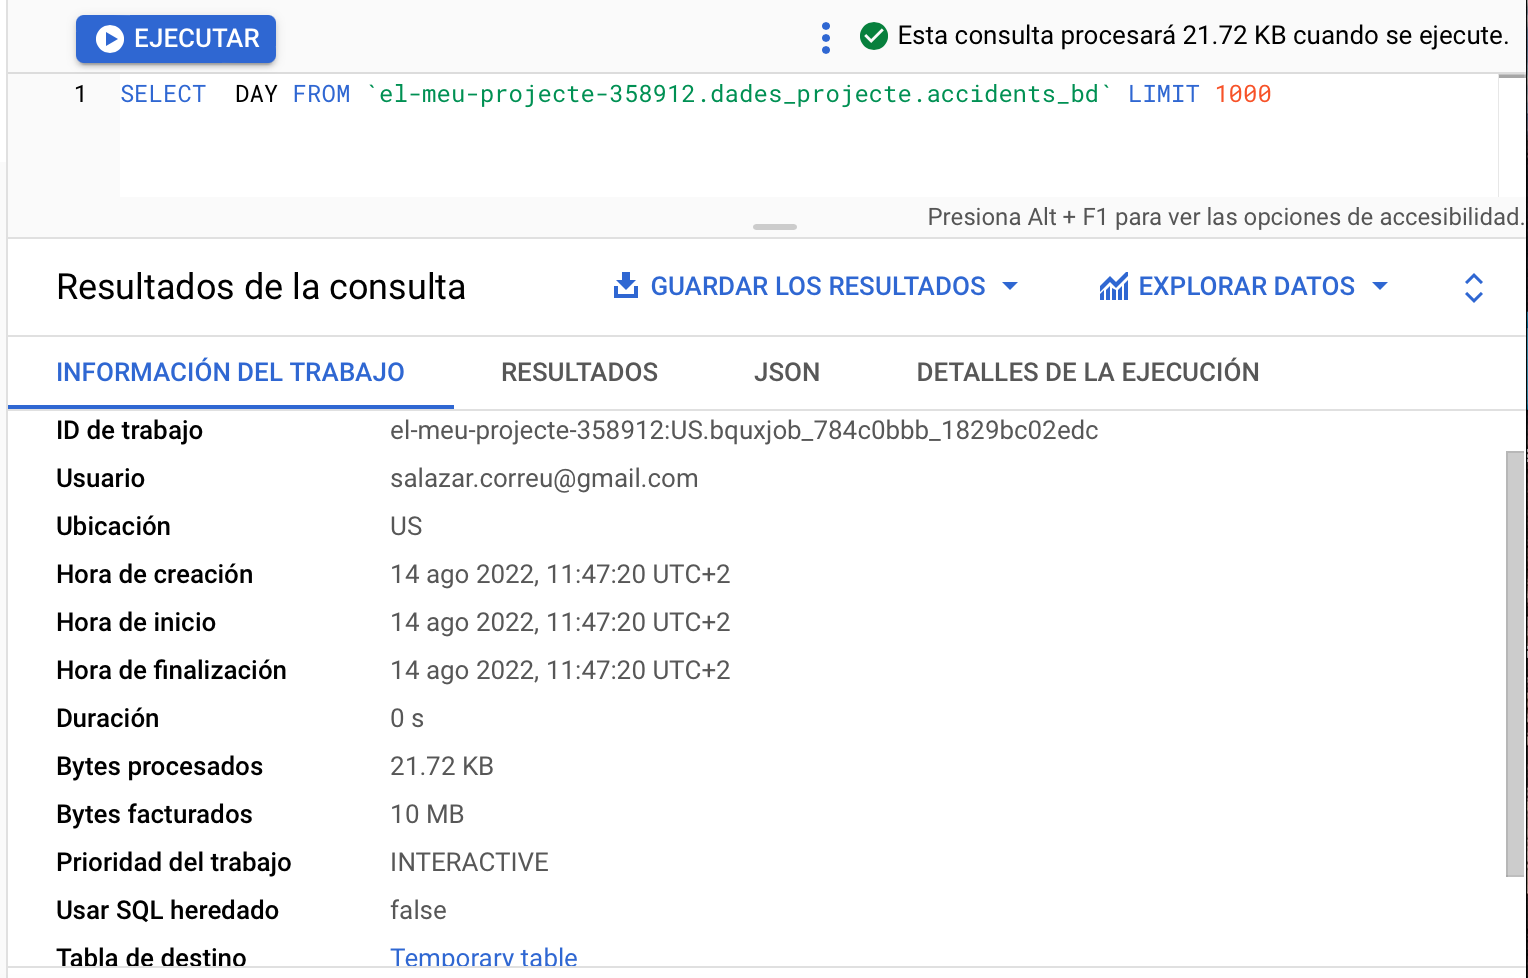
\includegraphics[width=10cm]{bq19}
\end{center}
\caption{Primera consulta}
\label{fig:bq19}
\end{figure}
\vspace{2mm}

Executarem aquesta consulta prement \verb|Executar|. Els resultats apareixen sota la finestra d'editor i mostra certs detalls com, per exemple, que s'ha executat en uns 0 segons per a mi. Per descomptat, podem desplaçar-nos i donar un cop d'ull a tots els resultats (a la dreta de la Figura ~\ref{fig:bq19}). Entre els detalls que es mostren per a cada consulta s'hi troben la informació del treball, els resultats en forma de taula, els resultats en format JSON i certs detalls de l'execució de la consulta. Si posem el focus en la informació del treball, es troba l'identificador d'aquest, l'usuari que l'ha executat, la ubicació on s'emmagatzemen les dades, l'hora de la creació i l'execució d'aquesta, el temps d'execució i els bytes processats i facturats. Veiem que el nombre de bytes facturats és de 10 MB, aquesta és la quantitat mínima que surt per defecte per a cada consulta per \textit{Google Cloud Platform}, i té en compte les despeses generals. Per a consultes a bases de dades més extenses, aquesta facturació serà major i ens impedirà l'ús de la zona de proves. L'última característica que crida l'atenció de la informació del treball és que els resultats s'emmagatzemen en una taula temporal. Això vol dir que aquesta taula resultant no es guardarà com una més en el nostre conjunt de dades i, per tant, no la podrem consultar.

\vspace{2mm}

\subsection{Creació d'una taula a partir d'un resultat de consulta}

Una altra alternativa a les taules temporals serà crear una taula en el nostre conjunt de dades a partir d'una taula temporal o vista. En aquest cas, farem una sèrie temporal de 31 observacions que ens compti el nombre d'accidents ocorreguts cada dia del mes a partir de la consulta següent:

\begin{verbatim}
SELECT DAY, COUNT(*) AS FREQ
FROM `el-meu-projecte-358912.dades_projecte.accidents_bd`
GROUP BY DAY
\end{verbatim}

Un cop realitzada la consulta, hem d'exportar totes aquestes dades a una nova taula i, per a fer-ho, revisarem algunes de les opcions d'exportació que es troben al menú \verb|Guardar resultats|. En aquest, apareixen diverses opcions per a la manera de guardar els resultats (Figura ~\ref{fig:bq17}). Podem guardar-los com un arxiu CSV en Google Drive o en un arxiu local. En el nostre cas, exportarem el contingut a una nova taula de BigQuery. Una vegada feta aquesta selecció, podem decidir el nom del projecte i el conjunt de dades on s'aprovisionarà la taula i, a més, establir un nom de taula. 

\vspace{2mm}
\begin{figure}[h!]
\par
\raisebox{-.5\height}{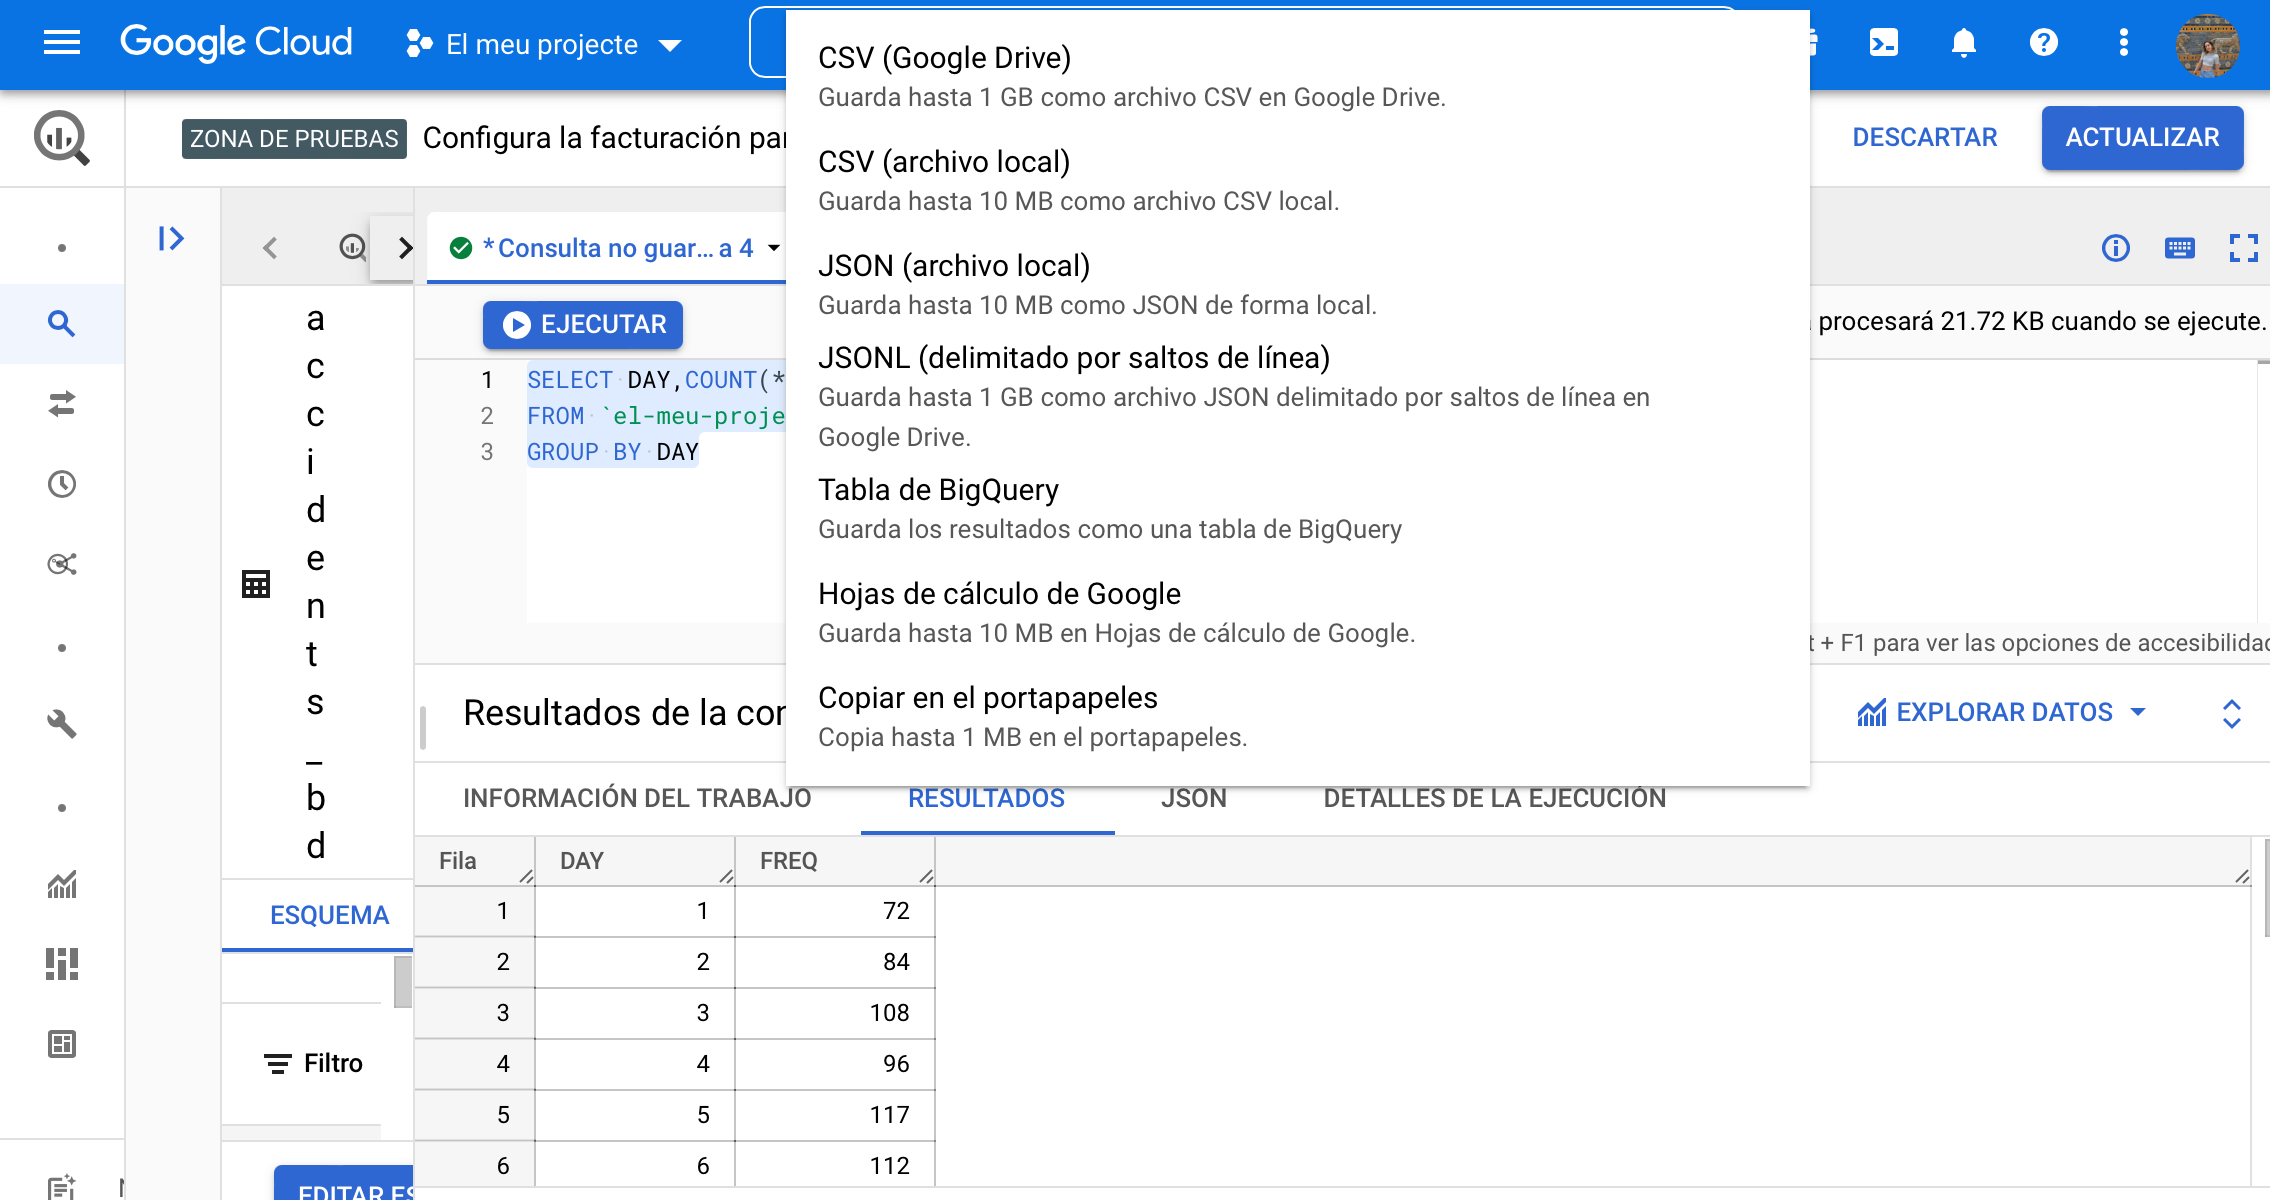
\includegraphics[width=7.25cm]{bq17}}%
\hfill
\raisebox{-.5\height}{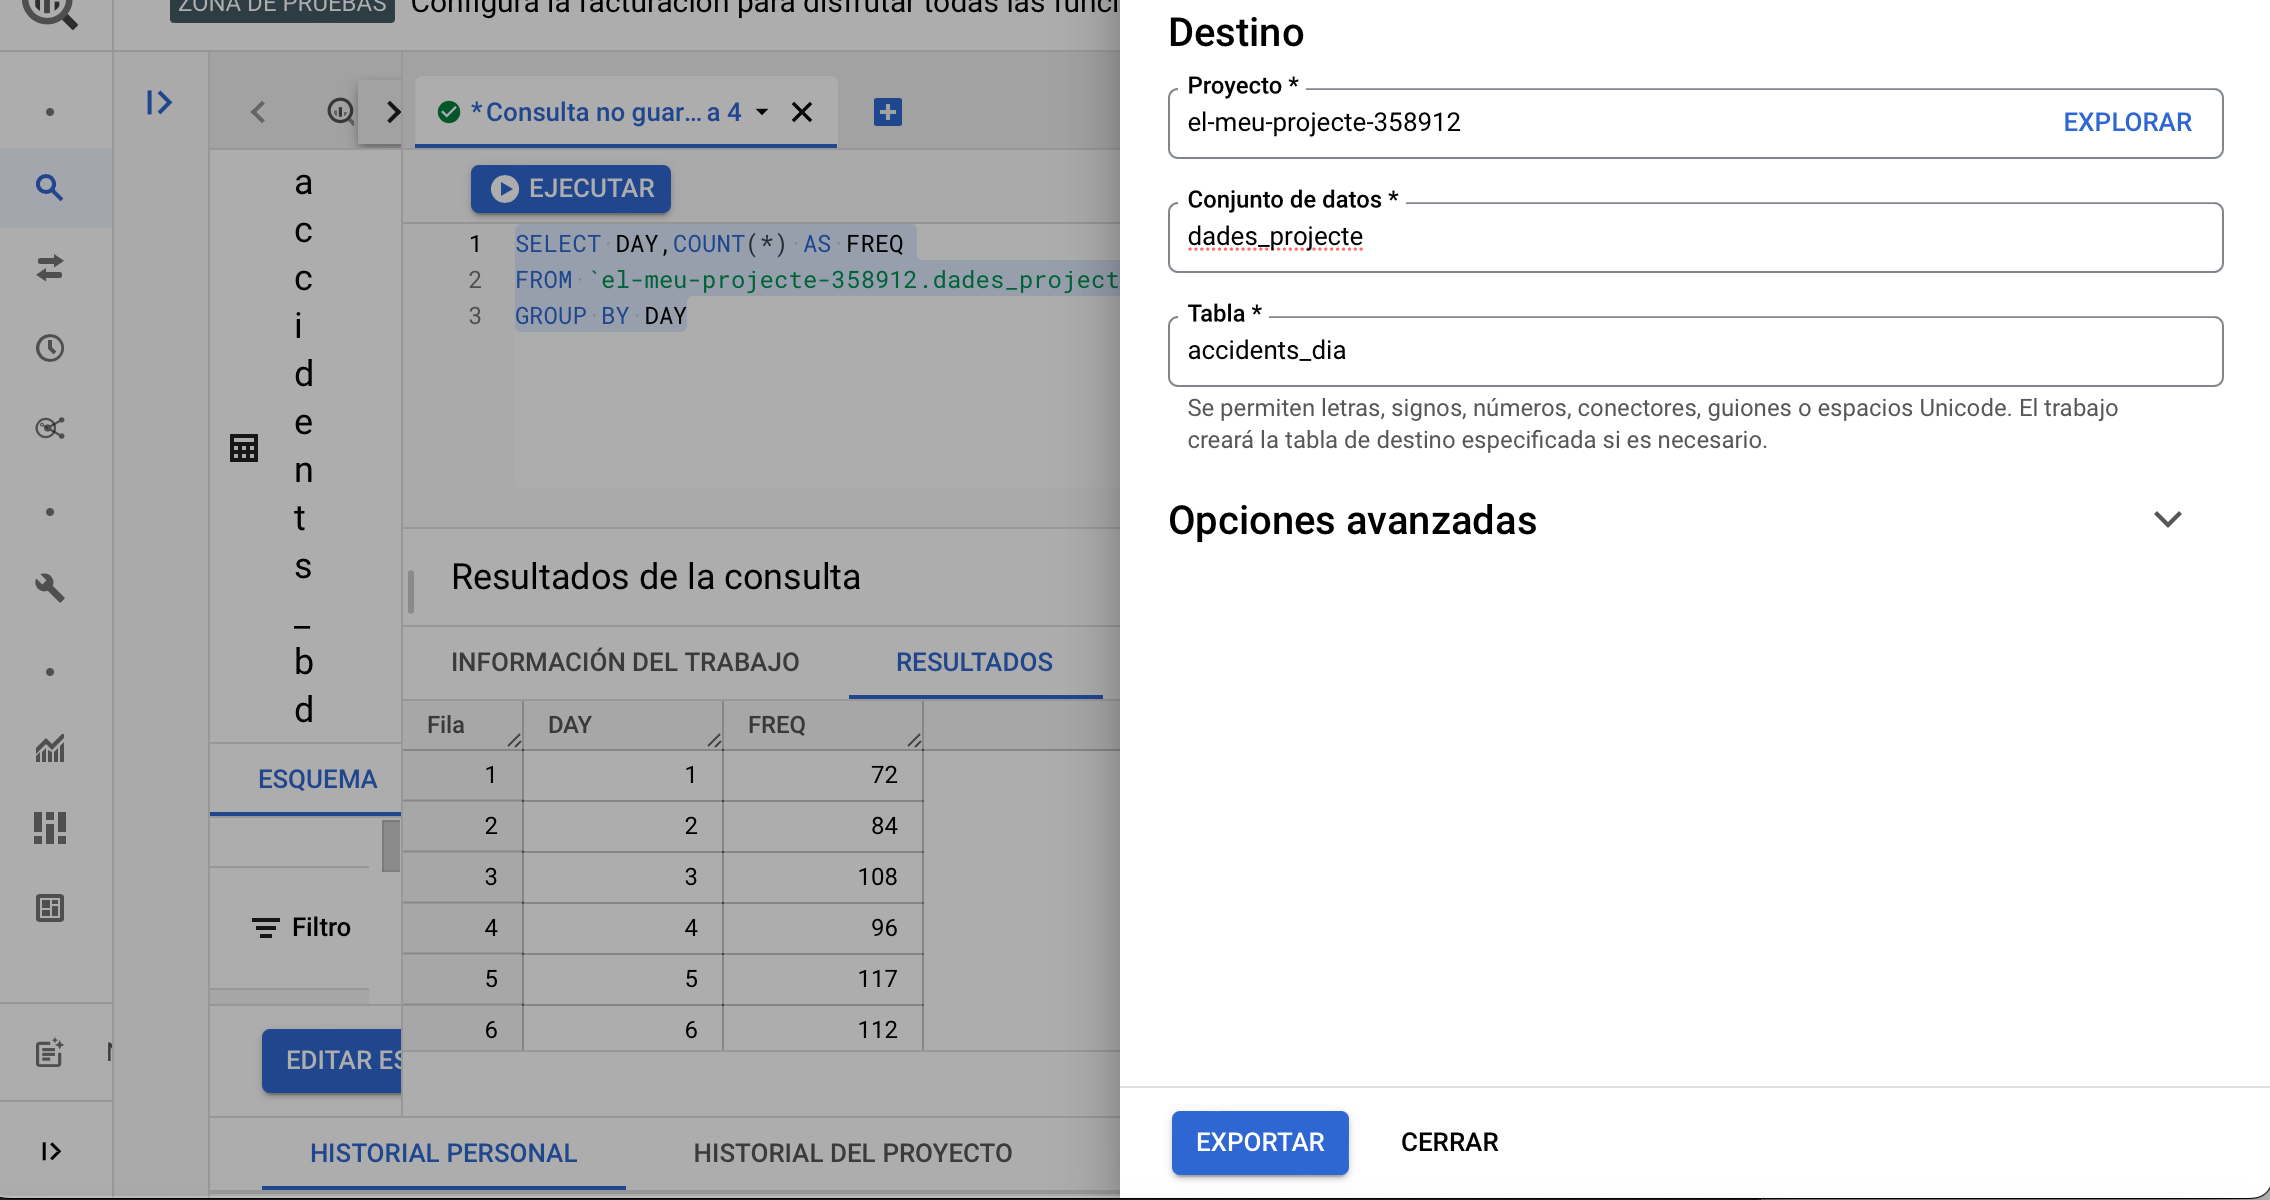
\includegraphics[width=7.25cm]{bq18}}%
\par

\caption{Creació d'una taula a partir d'una consulta}
\label{fig:bq17}
\end{figure}
\vspace{2mm}


Llavors, quan guardem les coses, això haurà iniciat un nou treball per a guardar la nova taula i carregar-la amb dades. Una vegada que tanquem aquesta notificació, podem treure el pin de l'Explorador i baix, apareix com una taula. En obrir-la confirmem que l'esquema apunta a les mateixes columnes que havíem referenciat en la clàusula \verb|SELECT| de la consulta que va crear aquesta taula. Des dels detalls podem confirmar que el nombre de files coincideix amb el dels resultats de la consulta, concretament 31. I després la vista prèvia ens mostrarà quines són les dades exactament. 

\vspace{2mm}

Hom es pot preguntar: \textit{Quina és la finalitat d'aquesta taula?} Bé, atès que només conté un subconjunt de la taula original, les consultes cap a aquesta taula tindran potencialment menys dades per a processar que les consultes que s'executen directament a la taula original. Potser en aquest cas no tornarem a necessitar aquesta consulta, però imaginem que només ens interessa estudiar els accidents que s'hagin produït a zones rurals i creem una consulta que filtri aquest tipus de casos. En aquesta situació, serà millor executar la resta de consultes sobre la taula petita, que inclou tota la informació que necessitem i probablement tindrà un cost de consulta menor.

\newpage

\section{Dades públiques i dades externes}

\subsection{Conjunts de dades públiques a BigQuery}

Mentre continuem familiaritzant-nos amb la plataforma, podem explorar una altra opció que ofereix BigQuery, que són dades que estan disponibles públicament per a que qualsevol usuari pugui executar les seves consultes. Aquests conjunts de dades públiques es troben en un projecte anomenat BigQuery Public Data. Per a accedir a elles, farem servir al botó d'agregació de dades (\verb|ADD DATA|), i escollirem l'opció que ens interessa (Figura ~\ref{fig:bq20}).

\vspace{2mm}
\begin{figure}[h!]
\begin{center}
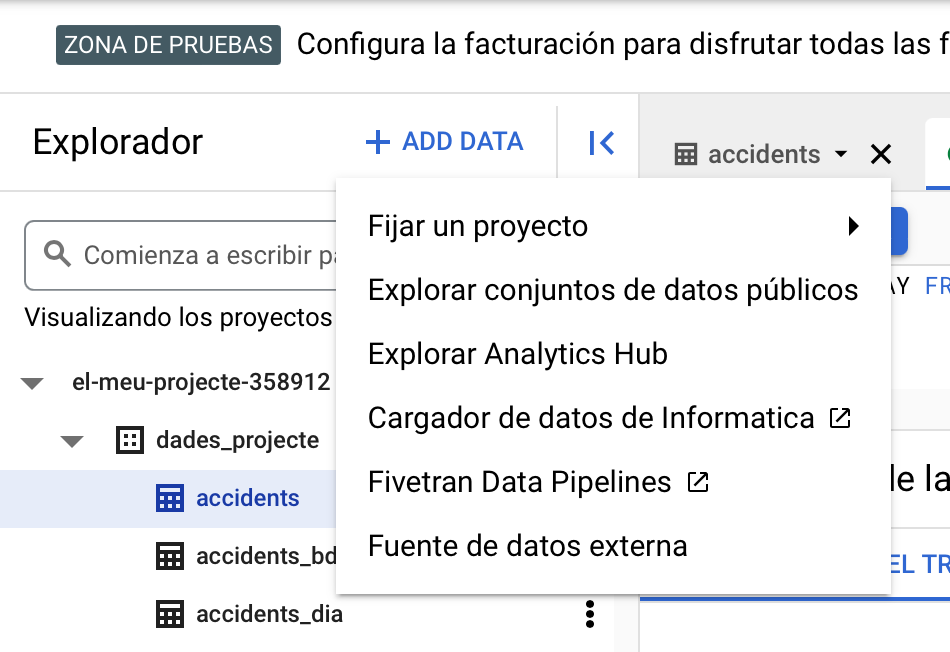
\includegraphics[width=10cm]{bq20}
\end{center}
\caption{Accés als conjunts de dades públiques}
\label{fig:bq20}
\end{figure}
\vspace{2mm}

Podem donar un cop d'ull als diferents conjunts de dades i taules d'aquest projecte i navegar entre les diferents opcions per a poder triar aquells que cridin la nostra atenció i amb els que treballarem. Per exemple, entre totes aquestes taules s'hi troba una que conté informació sobre la població catalana recopilada per l'aplicació \textit{GenCat Mobile Coverage} (Figura ~\ref{fig:bq21}). Dins d'aquesta taula s'hi troben dades recollides mitjançant \textit{crowdsourcing} i tenen informació sobre l'estat de la cobertura de la telefonia mòbil a Catalunya. La plataforma utilitza una aplicació Android per a registrar les dades dels ciutadans a través dels seus dispositius mòbils sobre el nivell de cobertura per operador, xarxa (2G, 3G i 4G) i la ubicació del dispositiu. Aquestes dades en concret van ser recopilades durant el període 2015-2017.

\vspace{2mm}
\begin{figure}[h!]
\par
\raisebox{-.5\height}{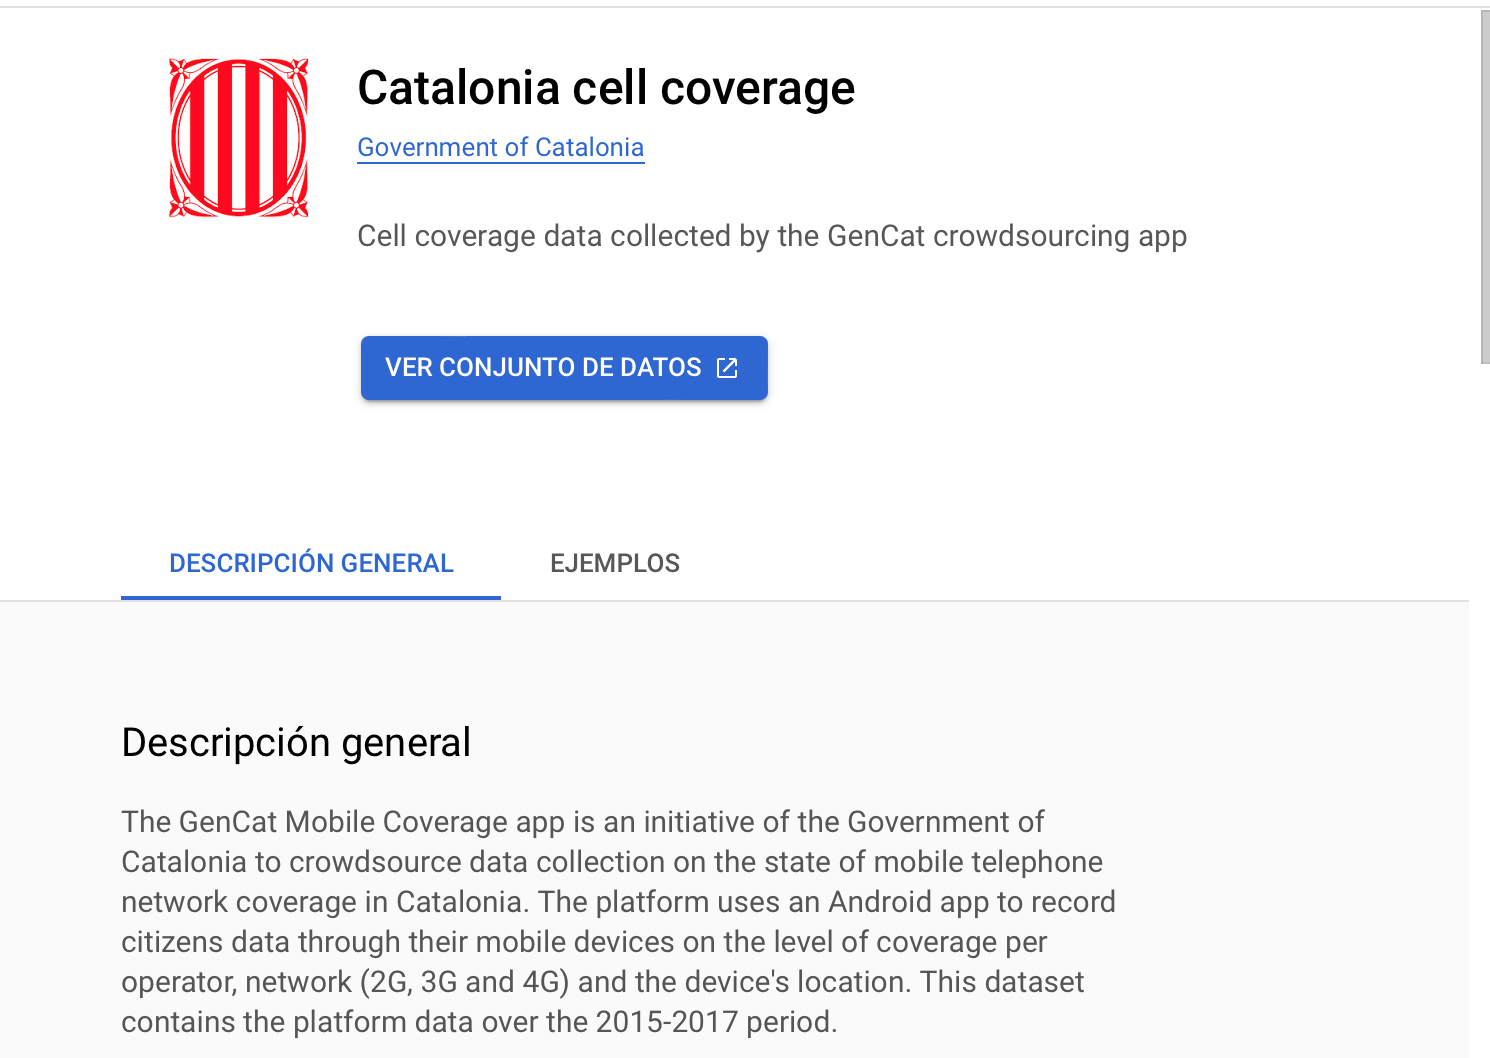
\includegraphics[width=7.25cm]{bq21}}%
\hfill
\raisebox{-.5\height}{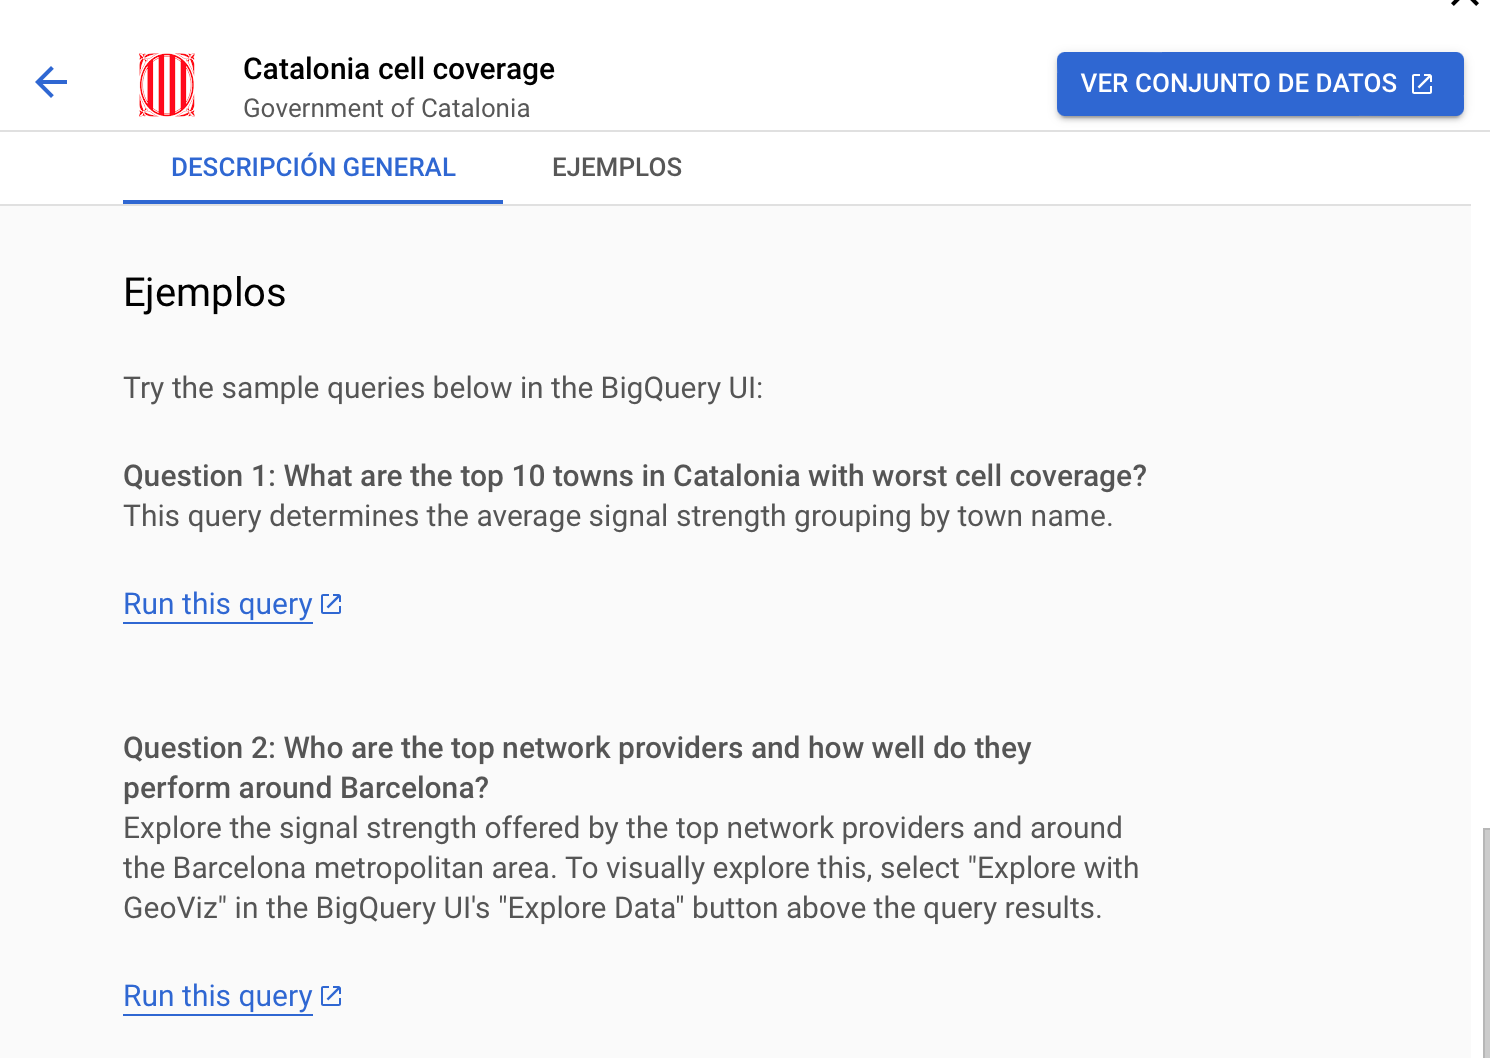
\includegraphics[width=7.25cm]{bq22}}%
\par

\caption{Creació d'una taula a partir d'una consulta}
\label{fig:bq21}
\end{figure}
\vspace{2mm}

Si volguéssim descarregar la taula i situar-la dins del nostre projecte, BigQuery ens permet aquesta operació si premem \textit{Visualitzar conjunt de dades} seguit de \textit{crear taula}. Això no obstant, també és possible consultar la taula sense necessitat de descarregar-la dins del nostre projecte, que és el que farem en aquest cas.

\vspace{2mm}

Dins la informació de la taula que ens proporciona la plataforma, apareix una secció amb consultes suggerides (a la dreta de la Figura ~\ref{fig:bq21}). D'entre aquestes, la primera fa referència als 10 pobles catalans amb pitjor cobertura de mòbil.  Si premem a \verb|Run this query|, el navegador ens redirigeix a l'editor amb la consulta preparada, i nosaltres la podem executar sense cap cost, ja que tant la taula com el resultat de la consulta estan emmagatzemats a BigQuery (Figura ~\ref{fig:bq23}).

\vspace{2mm}
\begin{figure}[h!]
\begin{center}
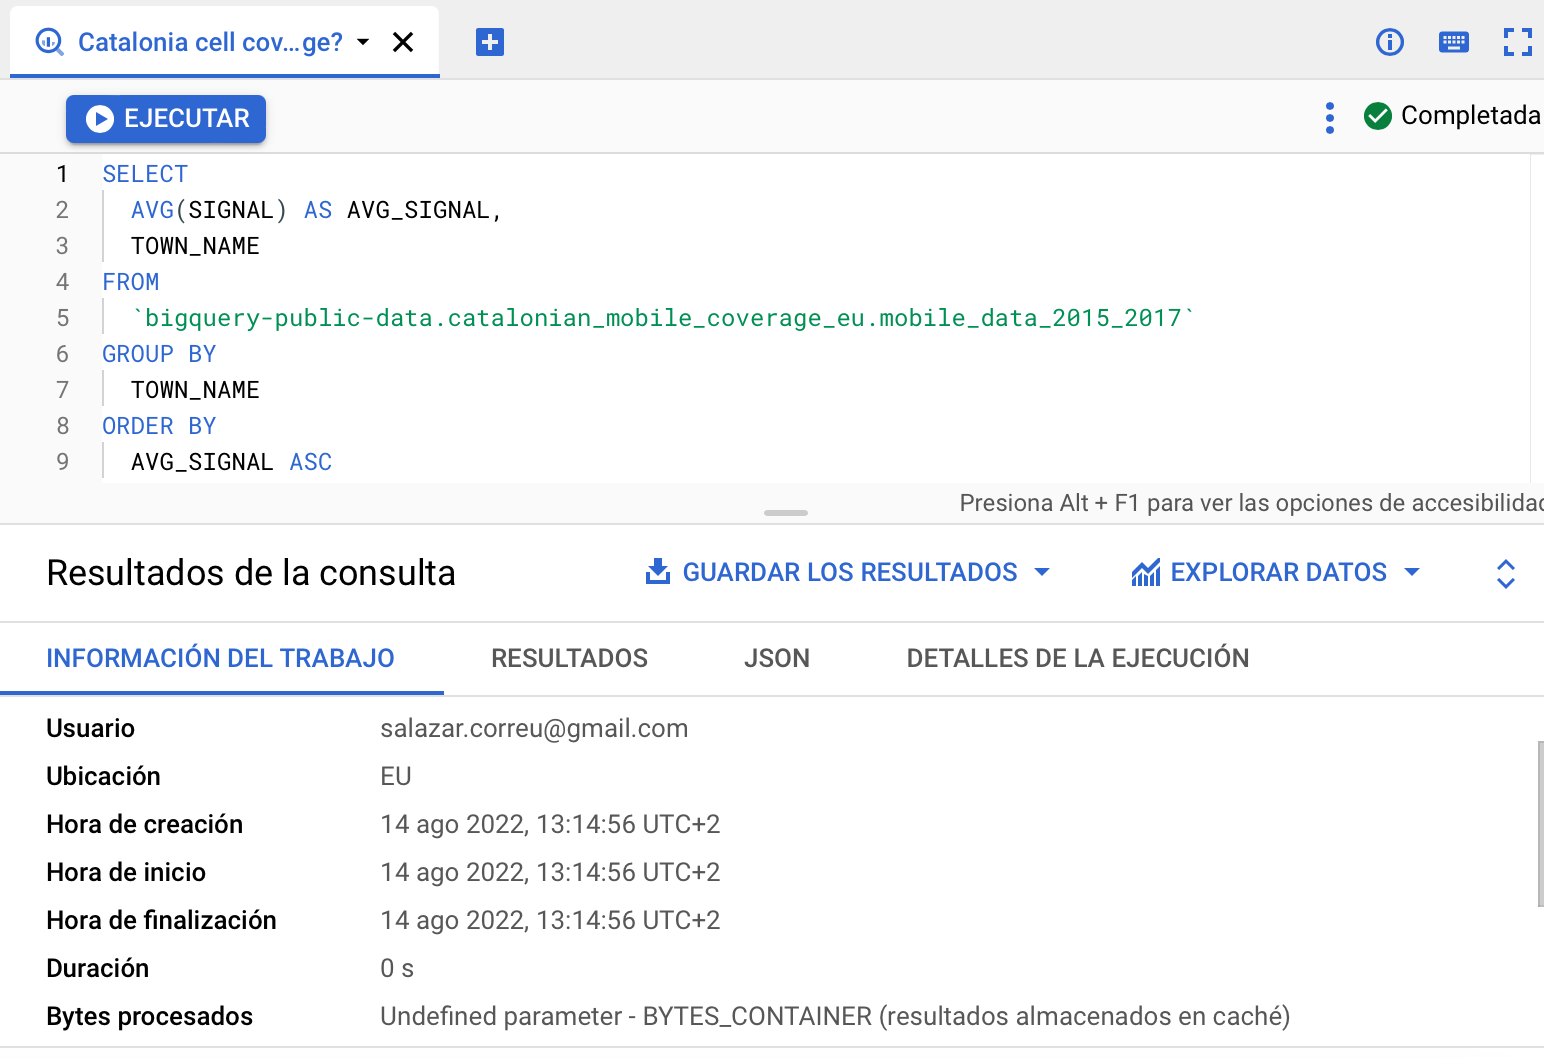
\includegraphics[width=10cm]{bq23}
\end{center}
\caption{Consulta a un conjunt de dades públic}
\label{fig:bq23}
\end{figure}
\vspace{2mm}

Els resultats d'aquesta consulta ens diu que els pobles catalans amb menys cobertura mòbil són Canejan, Boadella i les Escaules, Cabó, la Vajol, Gaià, Farrera, Gisclareny, Viver i Serrateix, Savallà del Comtat i Torroja del Priorat. A més, els bytes processats en aquesta consulta apareixen com un paràmetre indefinit, ja que aquests resultats estan emmagatzemats a la memòria cau de BigQuery.

\vspace{2mm}

Tal com hem vist, BigQuery emmagatzema a la seva memòria cau els resultats de la consulta perquè les dades puguin ser recuperades més ràpidament la pròxima vegada que s'executi la consulta. No obstant això, cal tenir en compte que només s'accedeix a les dades de la memòria cau quan s'executa la mateixa consulta després de la seva creació. Per exemple, si es modifiqués una mica aquesta consulta i, per exemple, demanés que em retornés tan sols el nom del poble en comptes d'aquest i la mitjana del senyal mòbil, podríem arribar a pensar que els resultats de la consulta d'aquesta execució haurien de retornar-nos un subconjunt de les dades que ja són presents en la memòria cau (ja que és un subconjunt de la nostra consulta anterior). Això no obstant, per la forma en què funciona la memòria cau de BigQuery, quan executem això, observarem que la informació no s'ha recuperat d'aquesta. En canvi, quan aquesta consulta es torna a executar, és quan la memòria cau s'activa, i és d'on es recuperen les dades. 

\vspace{2mm}

Per tant, la memòria cau només funciona si és la mateixa consulta la que es torna a executar. Aquestes característiques són de gran interès, ja que l'emmagatzematge en memòria cau és una gran manera de reduir el cost d'execució de les consultes, i també millora el rendiment d'aquestes. 

\subsection{Taules externes de BigQuery}

Una altra funció que presenta la plataforma és la lectura d'arxius externs que s'actualitzen de forma periòdica. Això és d'especial utilitat en els casos en què la informació de la qual es disposa és a temps real. Per a il·lustrar el funcionament de BigQuery en aquests casos, crearé una nova taula que estarà vinculada, en aquest cas, a \textit{Google Drive} (Figura ~\ref{fig:bq24}). És molt important que el propietari de la taula sigui el mateix compte que està vinculat a BigQuery, perquè en cas contrari sorgeix un missatge d'error.

\vspace{2mm}
\begin{figure}[h!]
\begin{center}
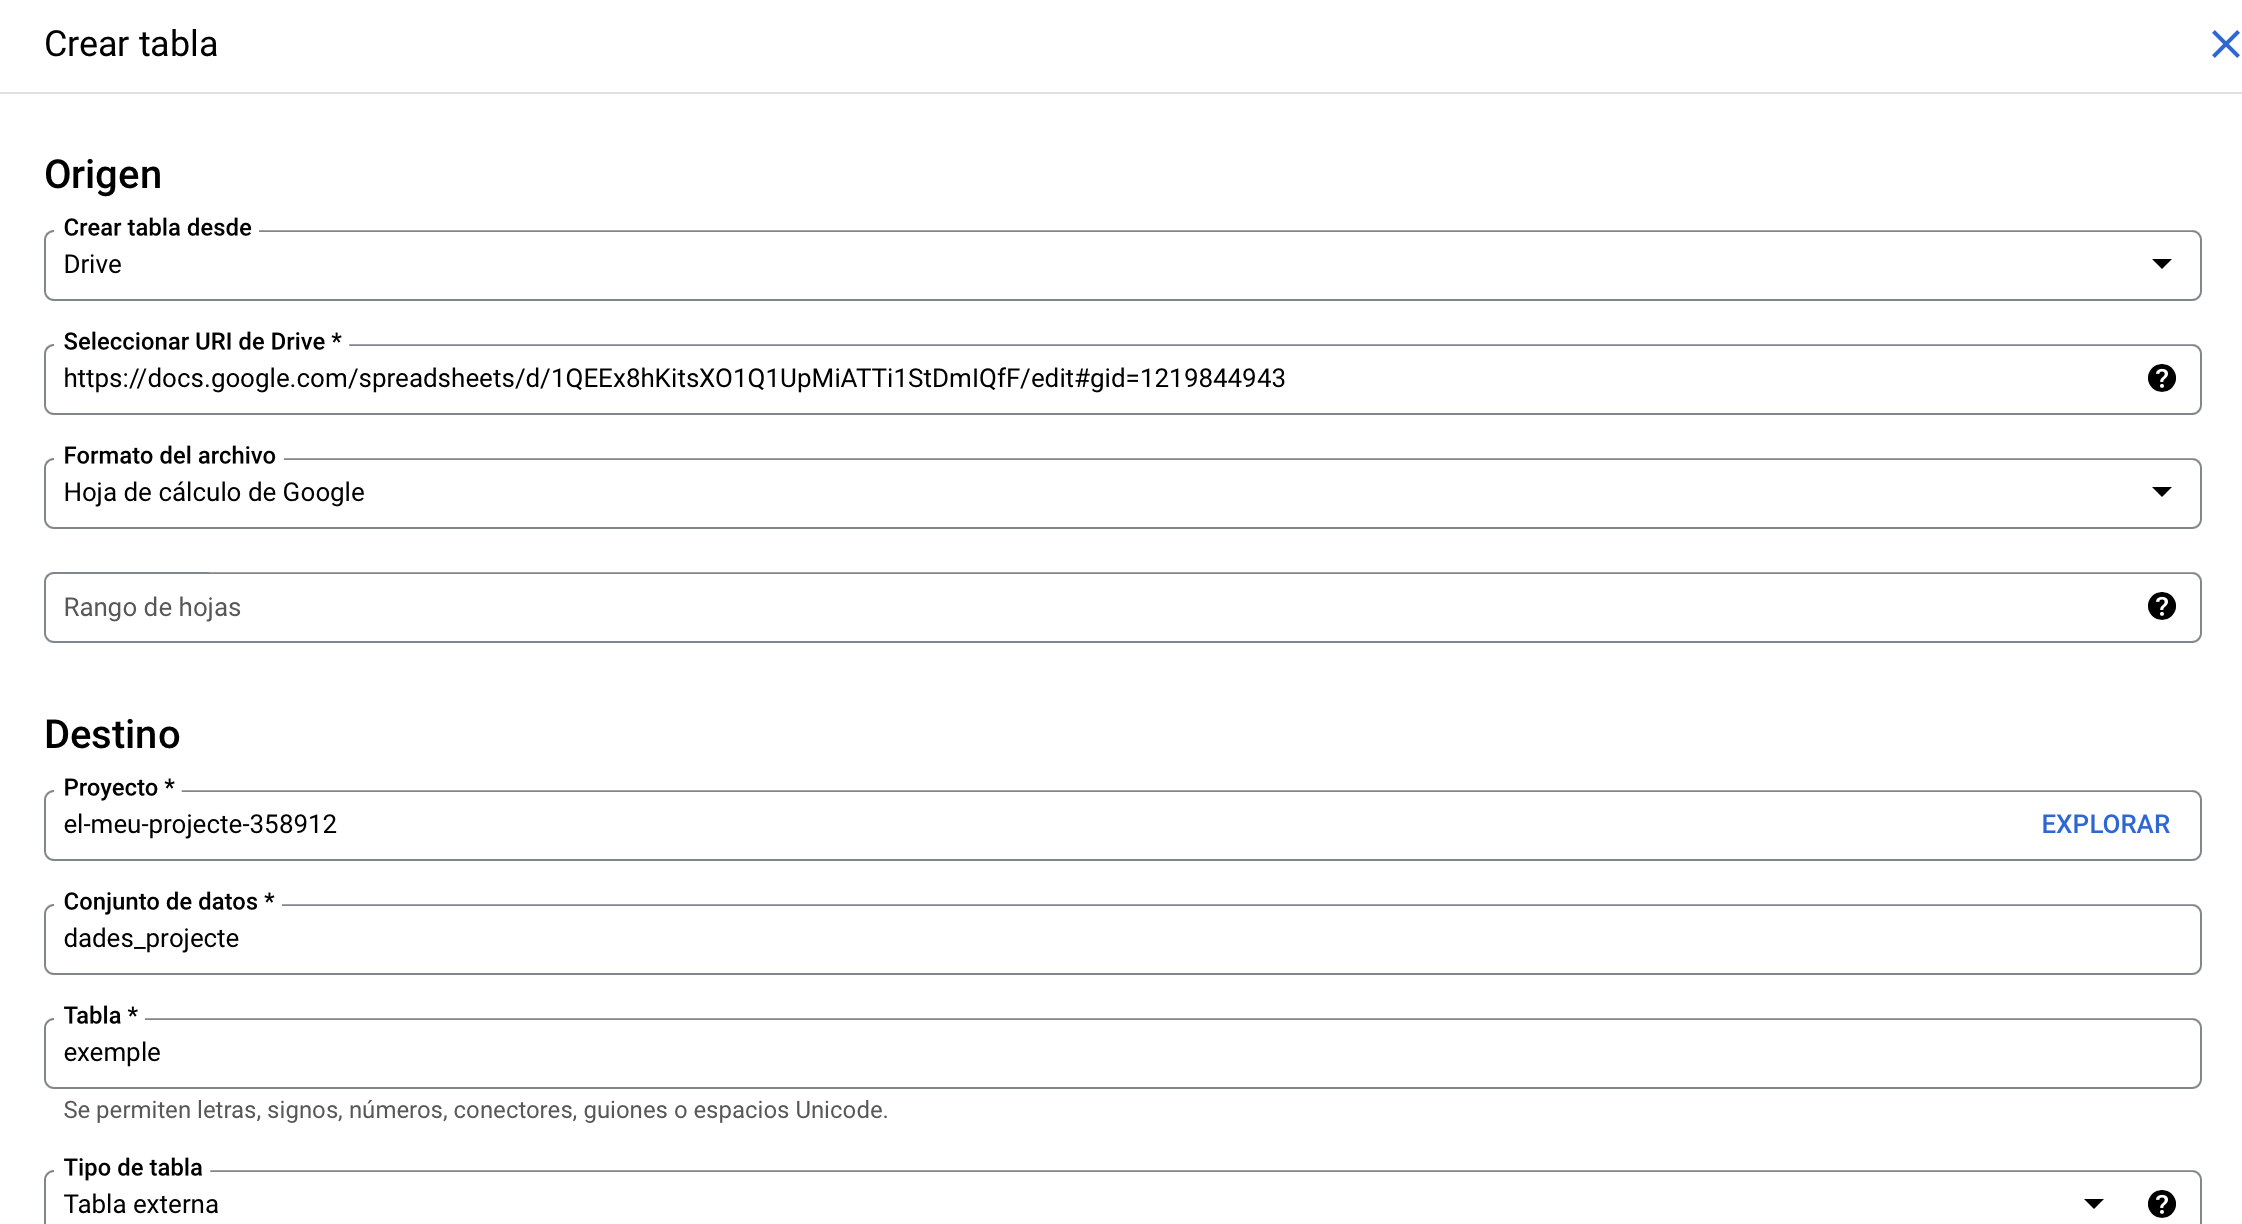
\includegraphics[width=10cm]{bq24}
\end{center}
\caption{Connexió a una taula externa}
\label{fig:bq24}
\end{figure}
\vspace{2mm}


Si ens dirigim als detalls, aquí és on veiem quelcom interessant. La grandària de la taula és de zero bytes, atès que les dades són externes a BigQuery (Figura ~\ref{fig:bq25}). Si ens desplacem, podem veure els detalls de les dades externes. Això significa que quan actualitzem el full de càlcul, qualsevol consulta cap a aquesta taula recollirà automàticament les dades més recents. Ja que la nostra consulta de la taula gran no és només una còpia del full de càlcul, sinó que és de fet una referència a ella. Parlant de consultar les dades, ens dirigirem a Query, i a obrir un editor de consultes en una nova pestanya. Quan una consulta s'executa, totes les dades són retornades a nosaltres, i podem accedir a elles com ho faríem amb qualsevol dada que resideixi en una taula nativa de BigQuery. 

\vspace{2mm}
\begin{figure}[h!]
\begin{center}
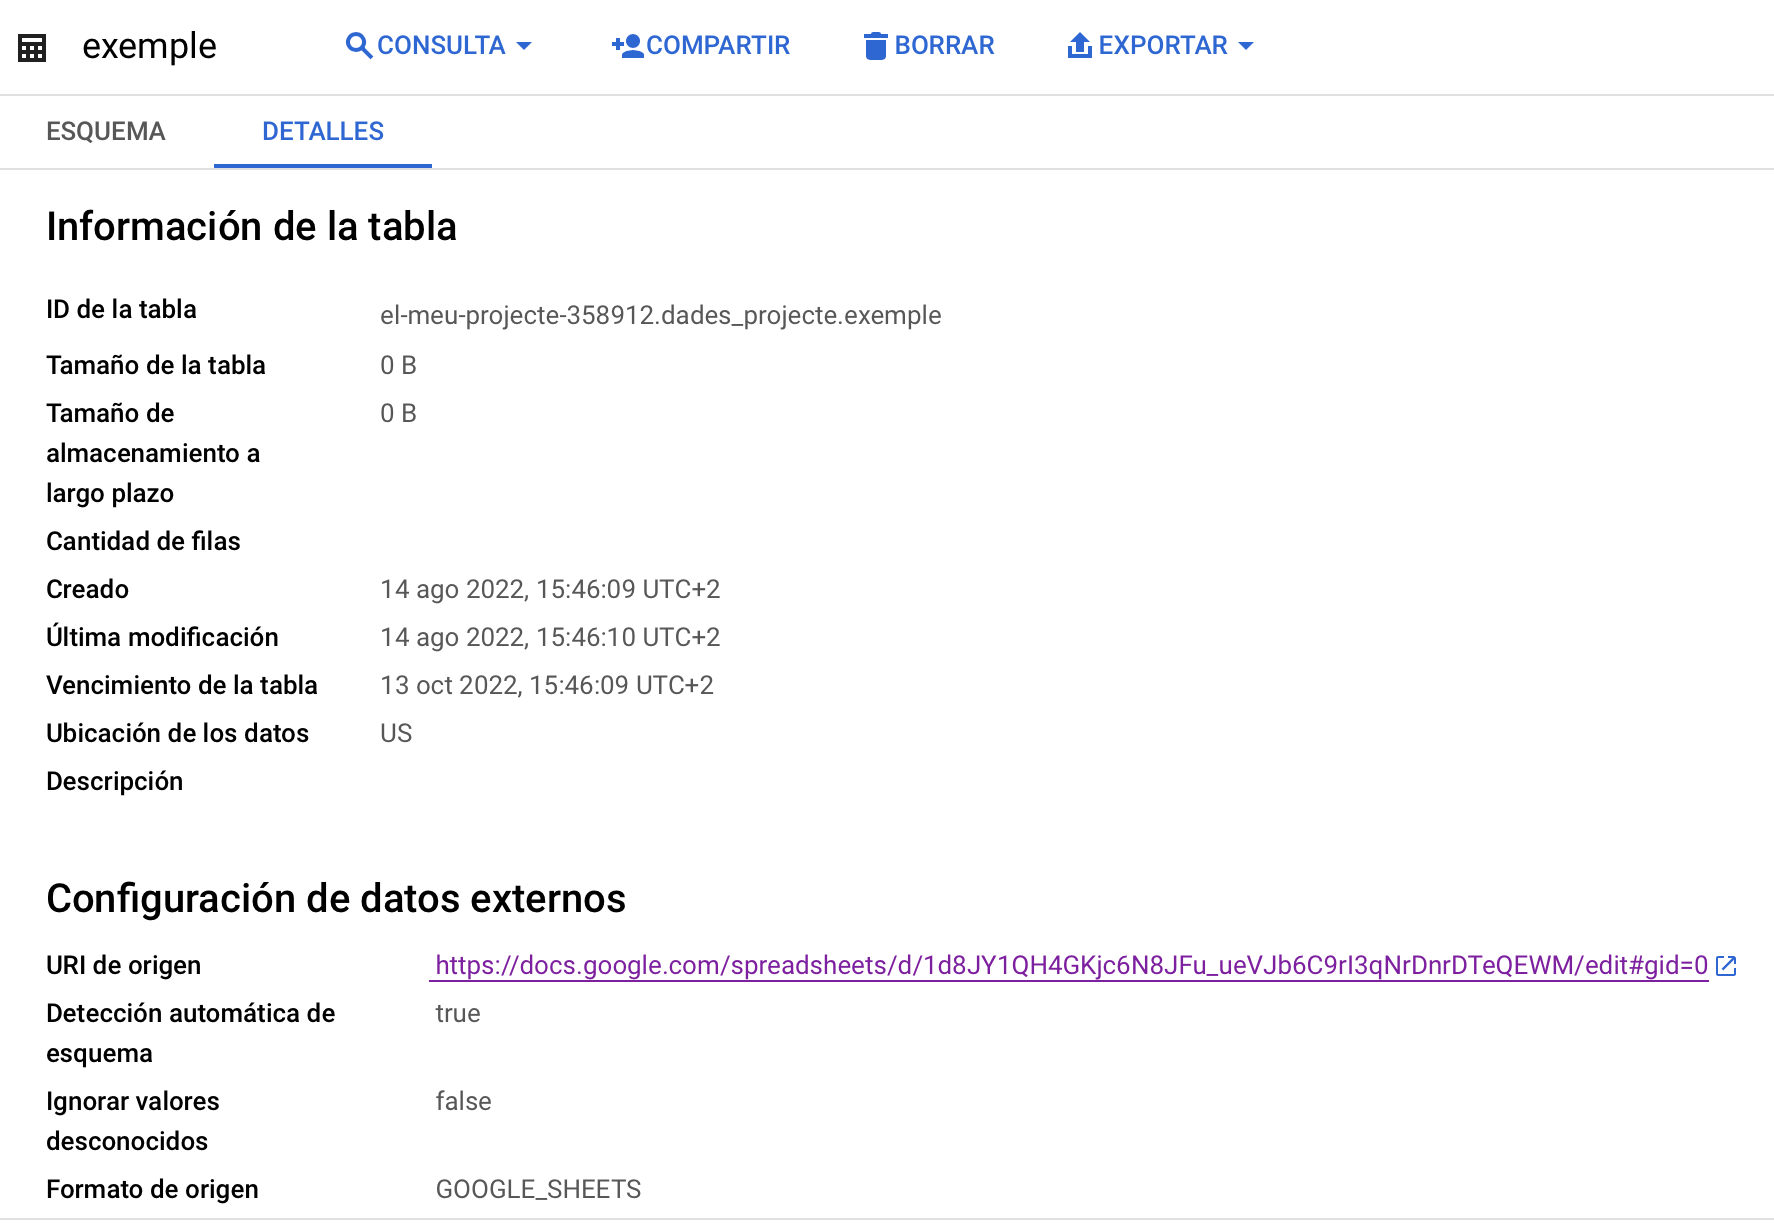
\includegraphics[width=10cm]{bq25}
\end{center}
\caption{Característiques d'una taula externa}
\label{fig:bq25}
\end{figure}
\vspace{2mm}

\newpage

\section{Integració de BigQuery amb Data Studio}

Ara que hem cobert els diferents tipus de taules de BigQuery, ens centrarem en com podem visualitzar les nostres consultes. 

\vspace{2mm}

Data Studio és una eina gratuïta que permet convertir les dades de les quals es disposa en panells o informes complets, fàcils de llegir, fàcils de compartir i totalment personalitzables. Algunes de les seves funcionalitats són:

\vspace{2mm}

- Descriure les dades amb gràfiques, que inclouen gràfics de línies, de barres i circulars, mapes geogràfics, gràfics d’àrea i de bombolles, taules de dades dinàmiques i molt més.

\vspace{2mm}

- Permet que els nostres informes siguin interactius amb filtres de visualització.

\vspace{2mm}

- Inclou enllaços i imatges en les quals es pot clicar per crear catàlegs de productes, biblioteques de vídeo i altres continguts amb URL.

\vspace{2mm}

- Facilita l’anotació i descripció dels informes amb text i imatges.

\vspace{2mm}

A més de presentar totes aquestes característiques, amb Data Studio es poden elaborar fàcilment informes sobre dades procedents d’una gran varietat de fonts, sense necessitat de programar. En tan sols uns instants, ens podem connectar a conjunts de dades com BigQuery.

\subsection{Ús de Data Studio des de BigQuery}

Imaginem que volem tornar a consultar el nombre d'accidents de trànsit que es van donar cada dia durant aquell mes als Estats Units. Per a fer aquesta consulta, farem servir la \textit{query} anterior:

\begin{verbatim}
SELECT DAY, COUNT(*) AS FREQ
FROM `el-meu-projecte-358912.dades_projecte.accidents_bd`
GROUP BY DAY
\end{verbatim}

Per a visualitzar la taula resultant, podem ampliar el menú \verb|Explorar dades|, tot seguit d'\verb|Explorar amb Data Studio| (Figura ~\ref{fig:bq26}).

\vspace{2mm}
\begin{figure}[h!]
\begin{center}
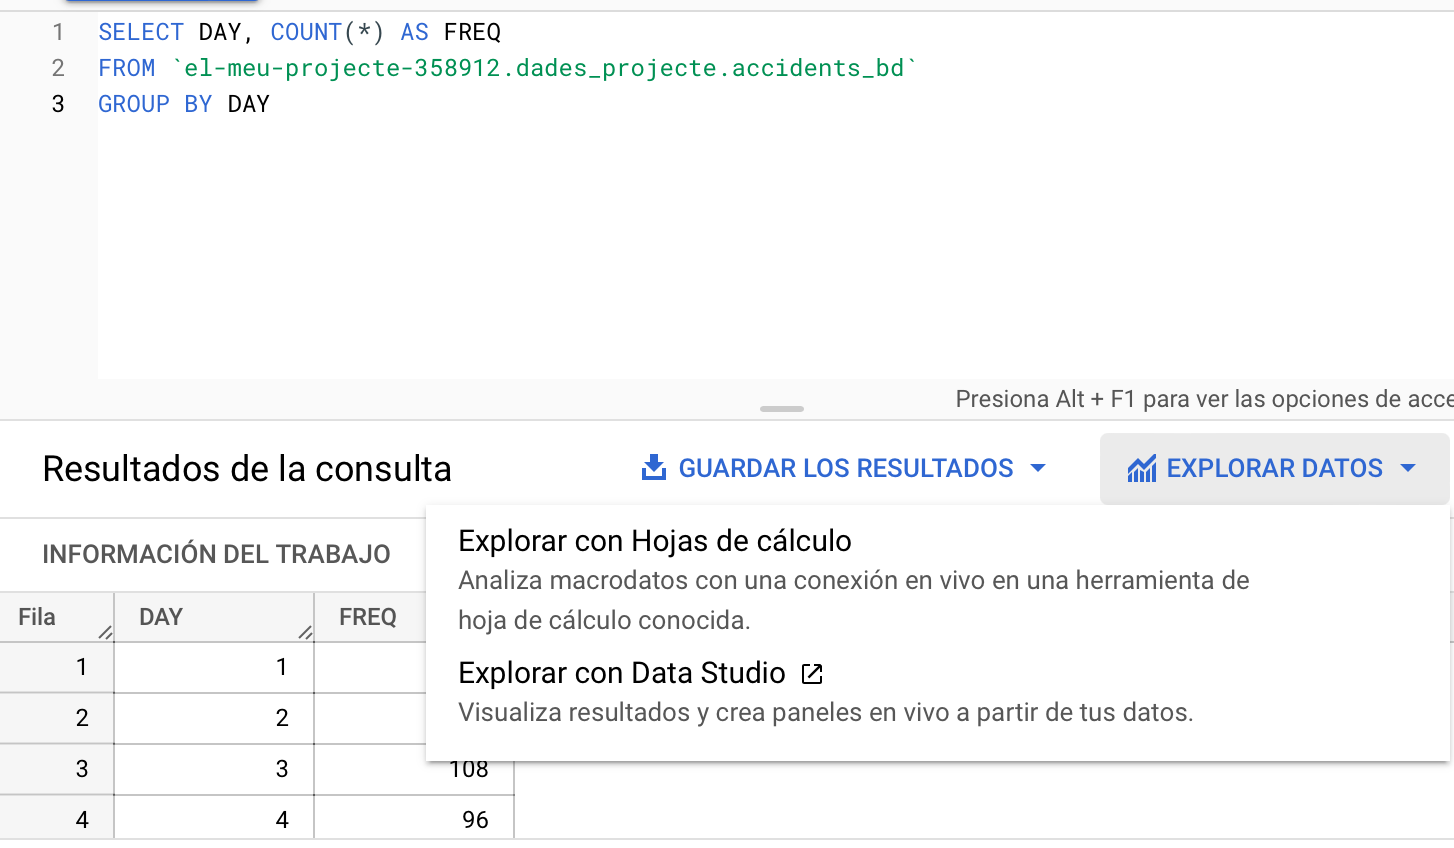
\includegraphics[width=10cm]{bq26}
\end{center}
\caption{Visualització d'una consulta a Data Studio}
\label{fig:bq26}
\end{figure}
\vspace{2mm}

Quan fem aquesta selecció, notaràs que ha sorgit una interfície, que ja té una taula que conté alguna informació agregada i un histograma amb la informació d'aquesta (Figura ~\ref{fig:bq27}).

\vspace{2mm}
\begin{figure}[h!]
\begin{center}
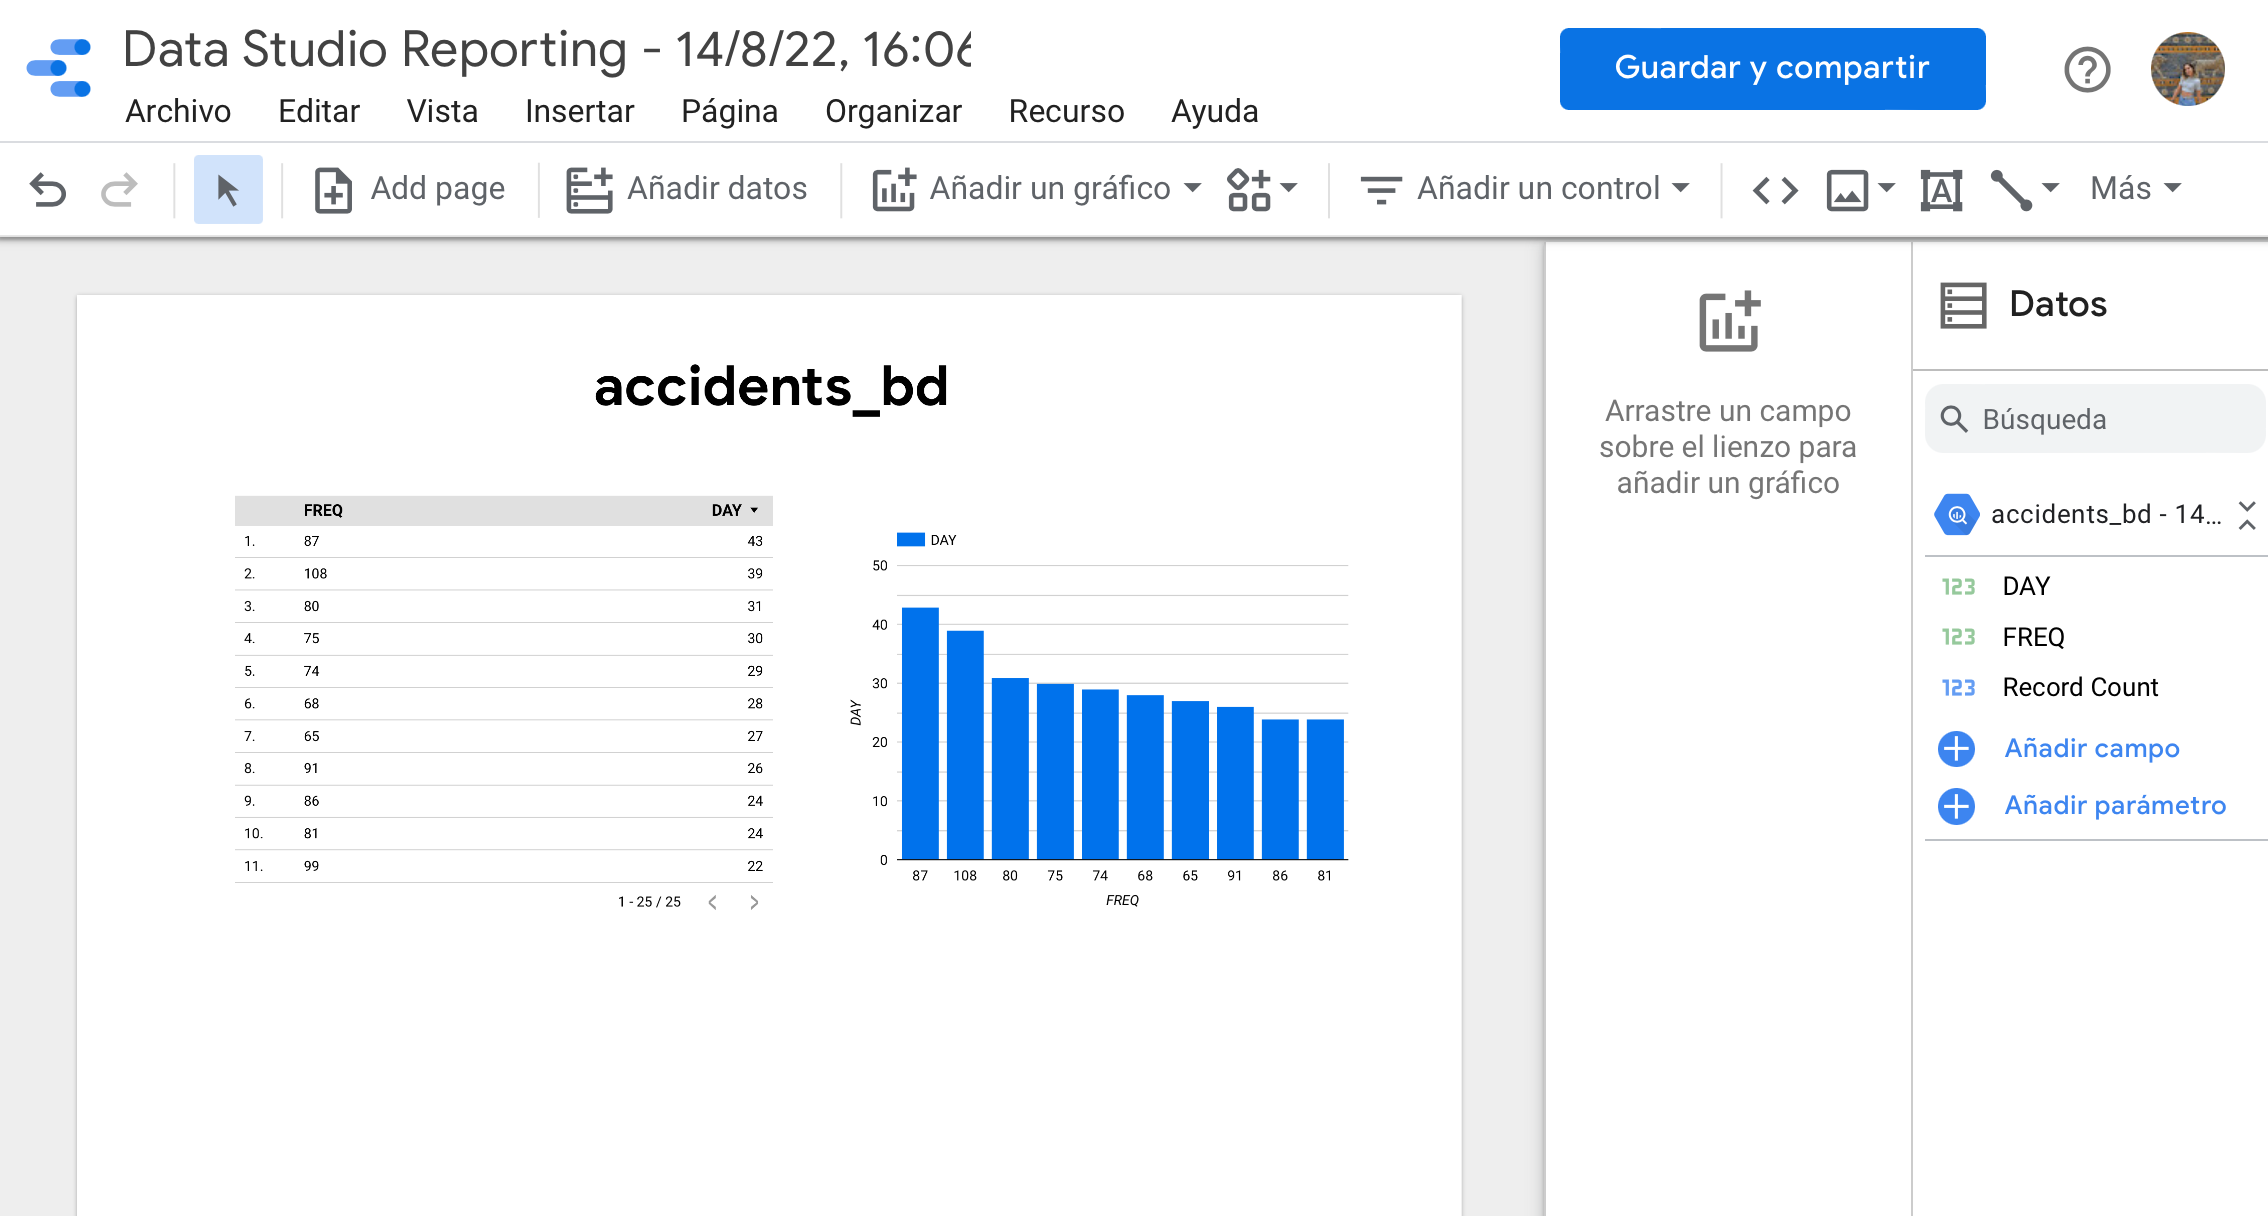
\includegraphics[width=10cm]{bq27}
\end{center}
\caption{Consulta des de Data Studio}
\label{fig:bq27}
\end{figure}
\vspace{2mm}

Data Studio, per defecte, ha entès que una taula de recompte es visualitza normalment a partir d'un \textit{bar plot} o histograma, i per això l'ha creat sense que nosaltres ho hàgim especificat. Així i tot, nosaltres podem seleccionar una visualització abans de configurar-la per a presentar la informació que necessitem. Pose'm-nos en el cas que preferim un gràfic de barres per a la visualització d'aquestes dades. Premem l'opció \verb|Afegir un gràfic| i ens assegurem que la dimensió, que en aquest cas són els dies, i la mètrica, la freqüència dels accidents, estiguin seleccionades segons el que vulguem representar (Figura ~\ref{fig:bq28}). 

\vspace{2mm}
\begin{figure}[h!]
\par
\raisebox{-.5\height}{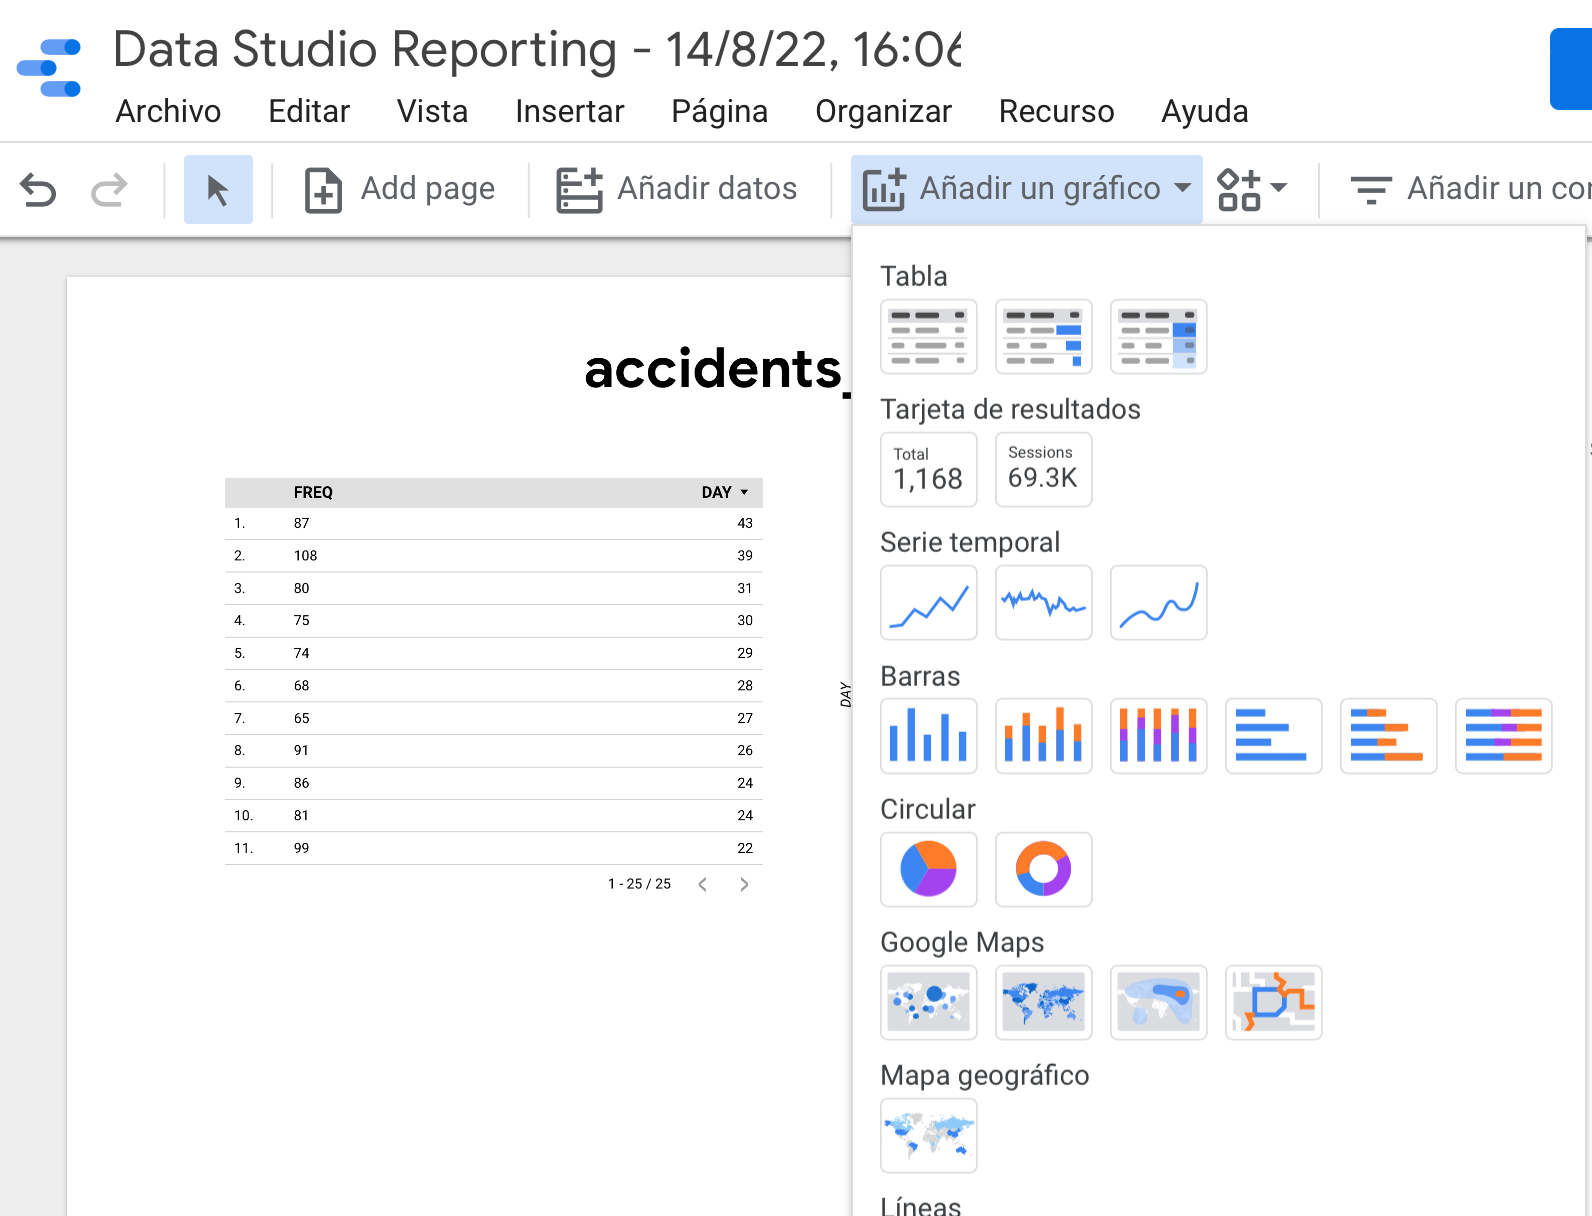
\includegraphics[width=7.25cm]{bq28}}%
\hfill
\raisebox{-.5\height}{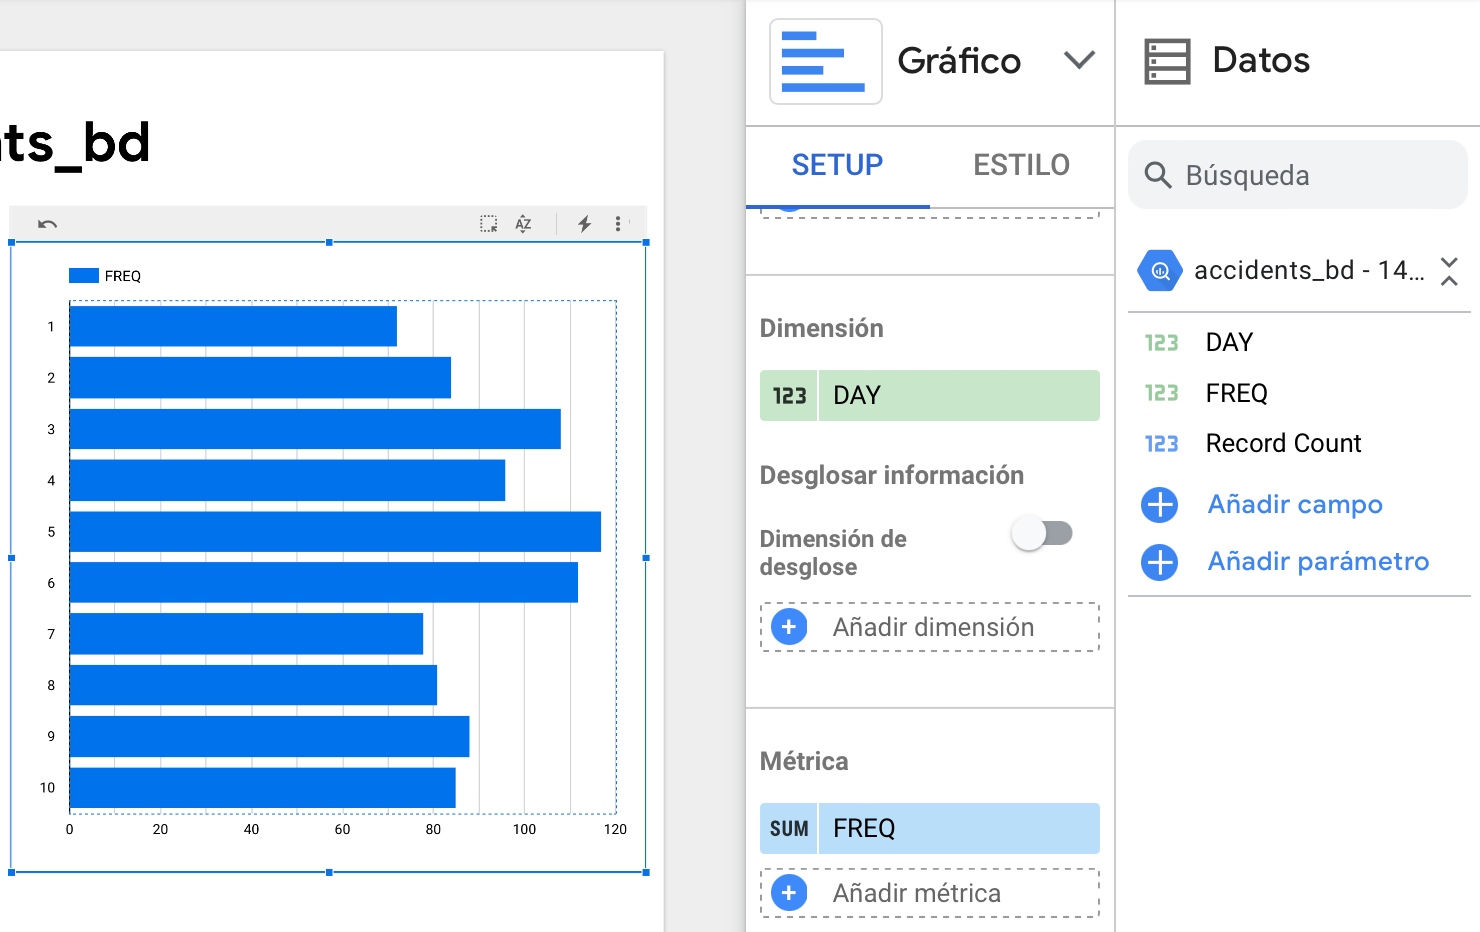
\includegraphics[width=7.25cm]{bq29}}%
\par

\caption{Creació d'un gràfic a partir de Data Studio}
\label{fig:bq28}
\end{figure}
\vspace{2mm}

\subsection{Ús de Data Studio des de la pròpia plataforma}

Per a utilitzar aquesta eina és necessari disposar d’un compte a Google. Per accedir a la pàgina, navega \href{https://datastudio.google.com}{aquí} i inicia sessió amb el teu compte. Un cop dins de Data Studio, veuràs una pantalla d’inici amb les característiques següents:

\vspace{2mm}
\begin{figure}[h!]
\begin{center}
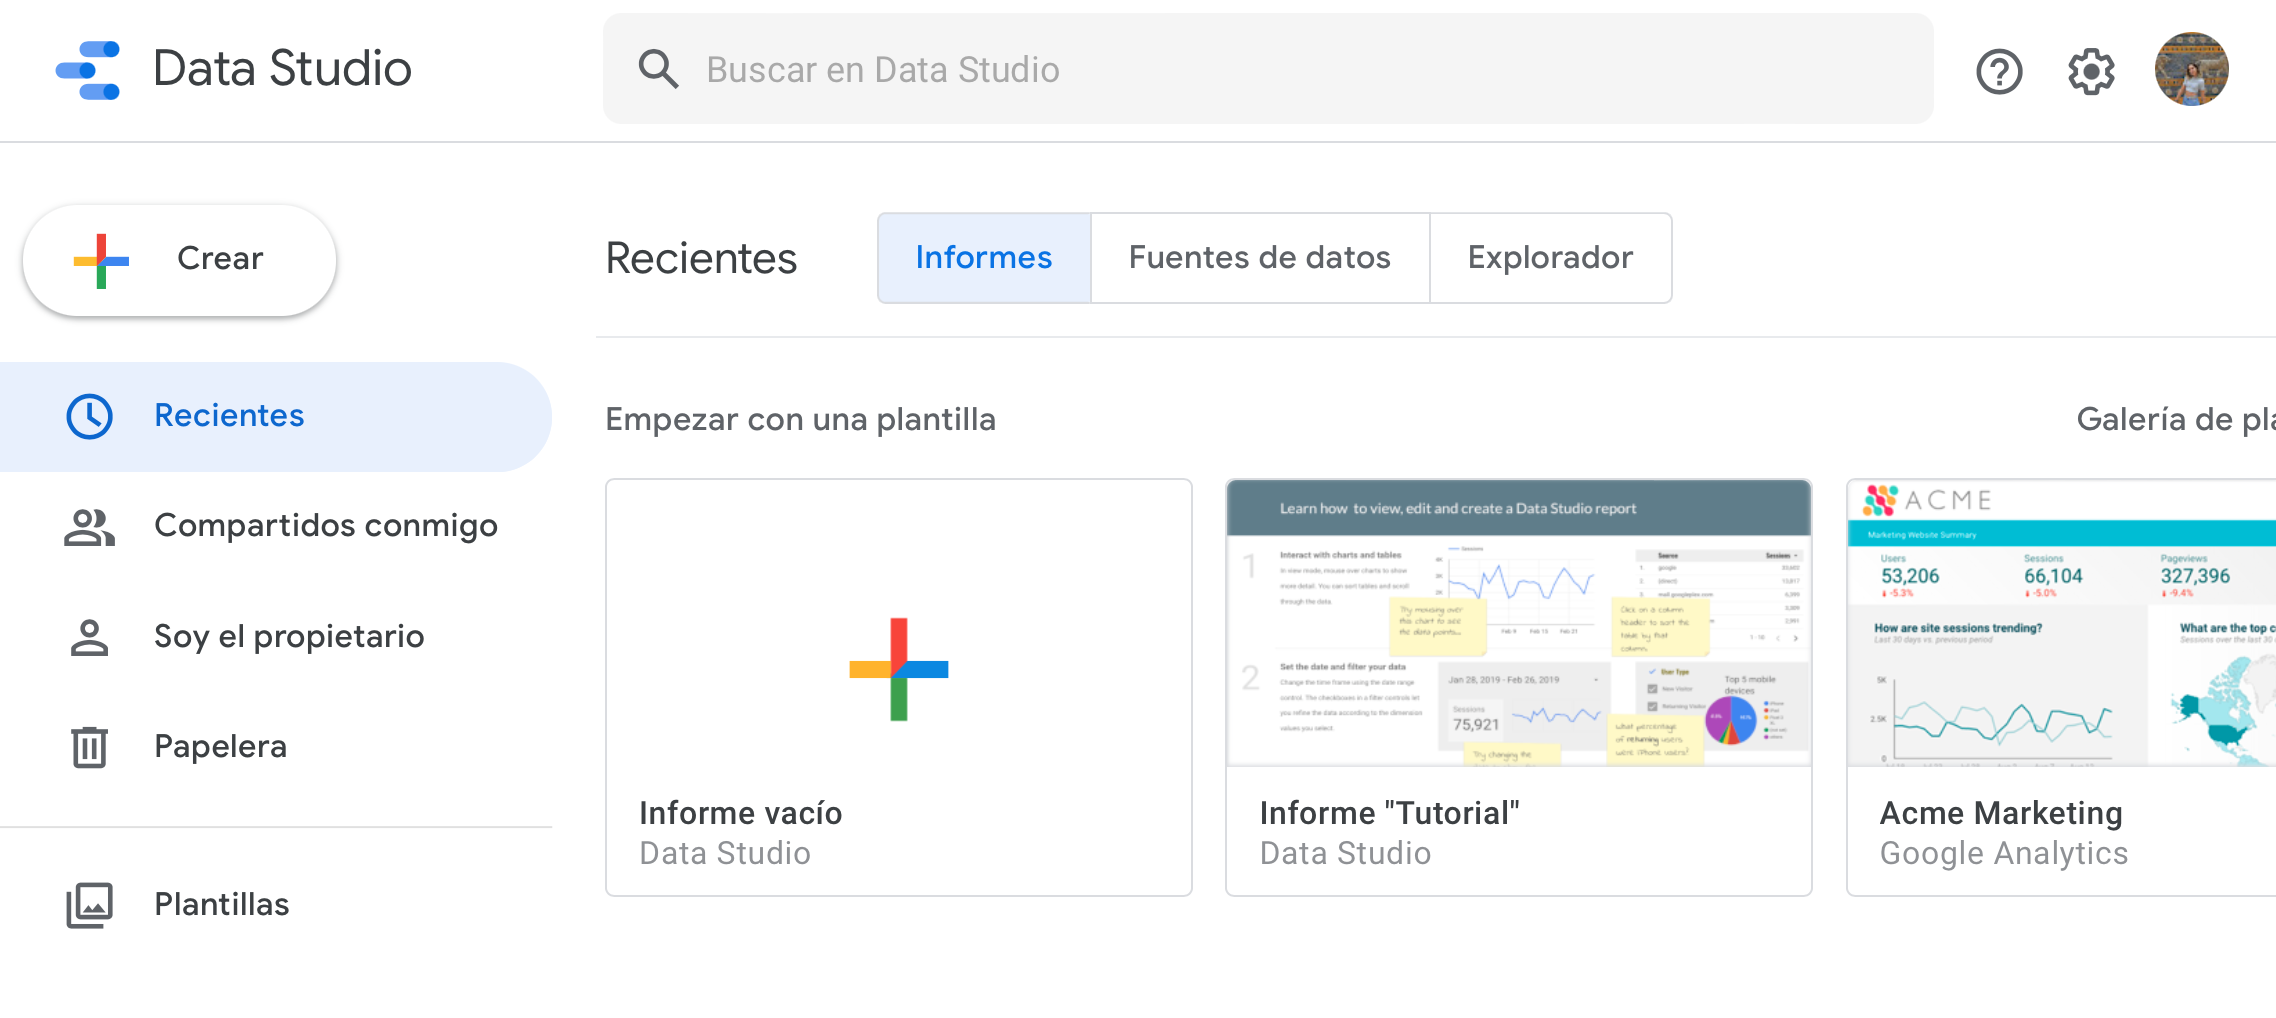
\includegraphics[width=10cm]{ds1}
\end{center}
\caption{Inici de Data Studio}
\label{fig:ds1}
\end{figure}
\vspace{2mm}

A la pàgina d’inici hi ha una sèrie de plantilles, que són una forma entretinguda d’explorar les capacitats de Data Studio. En el nostre cas, com el que ens interessa és crear un informe des de zero, clicarem a \verb|Informe vacío|. Un cop dins l’informe en blanc, s’hauran d’afegir les dades que volem representar en aquest (Figura ~\ref{fig:ds2}). Tenim moltes opcions a l'hora d'escollir la font de les dades, però per a fer-ho més senzill vincularem l'informe a BigQuery, específicament al nostre conjunt de dades \verb|accidents_bd|.

\vspace{2mm}
\begin{figure}[h!]
\begin{center}
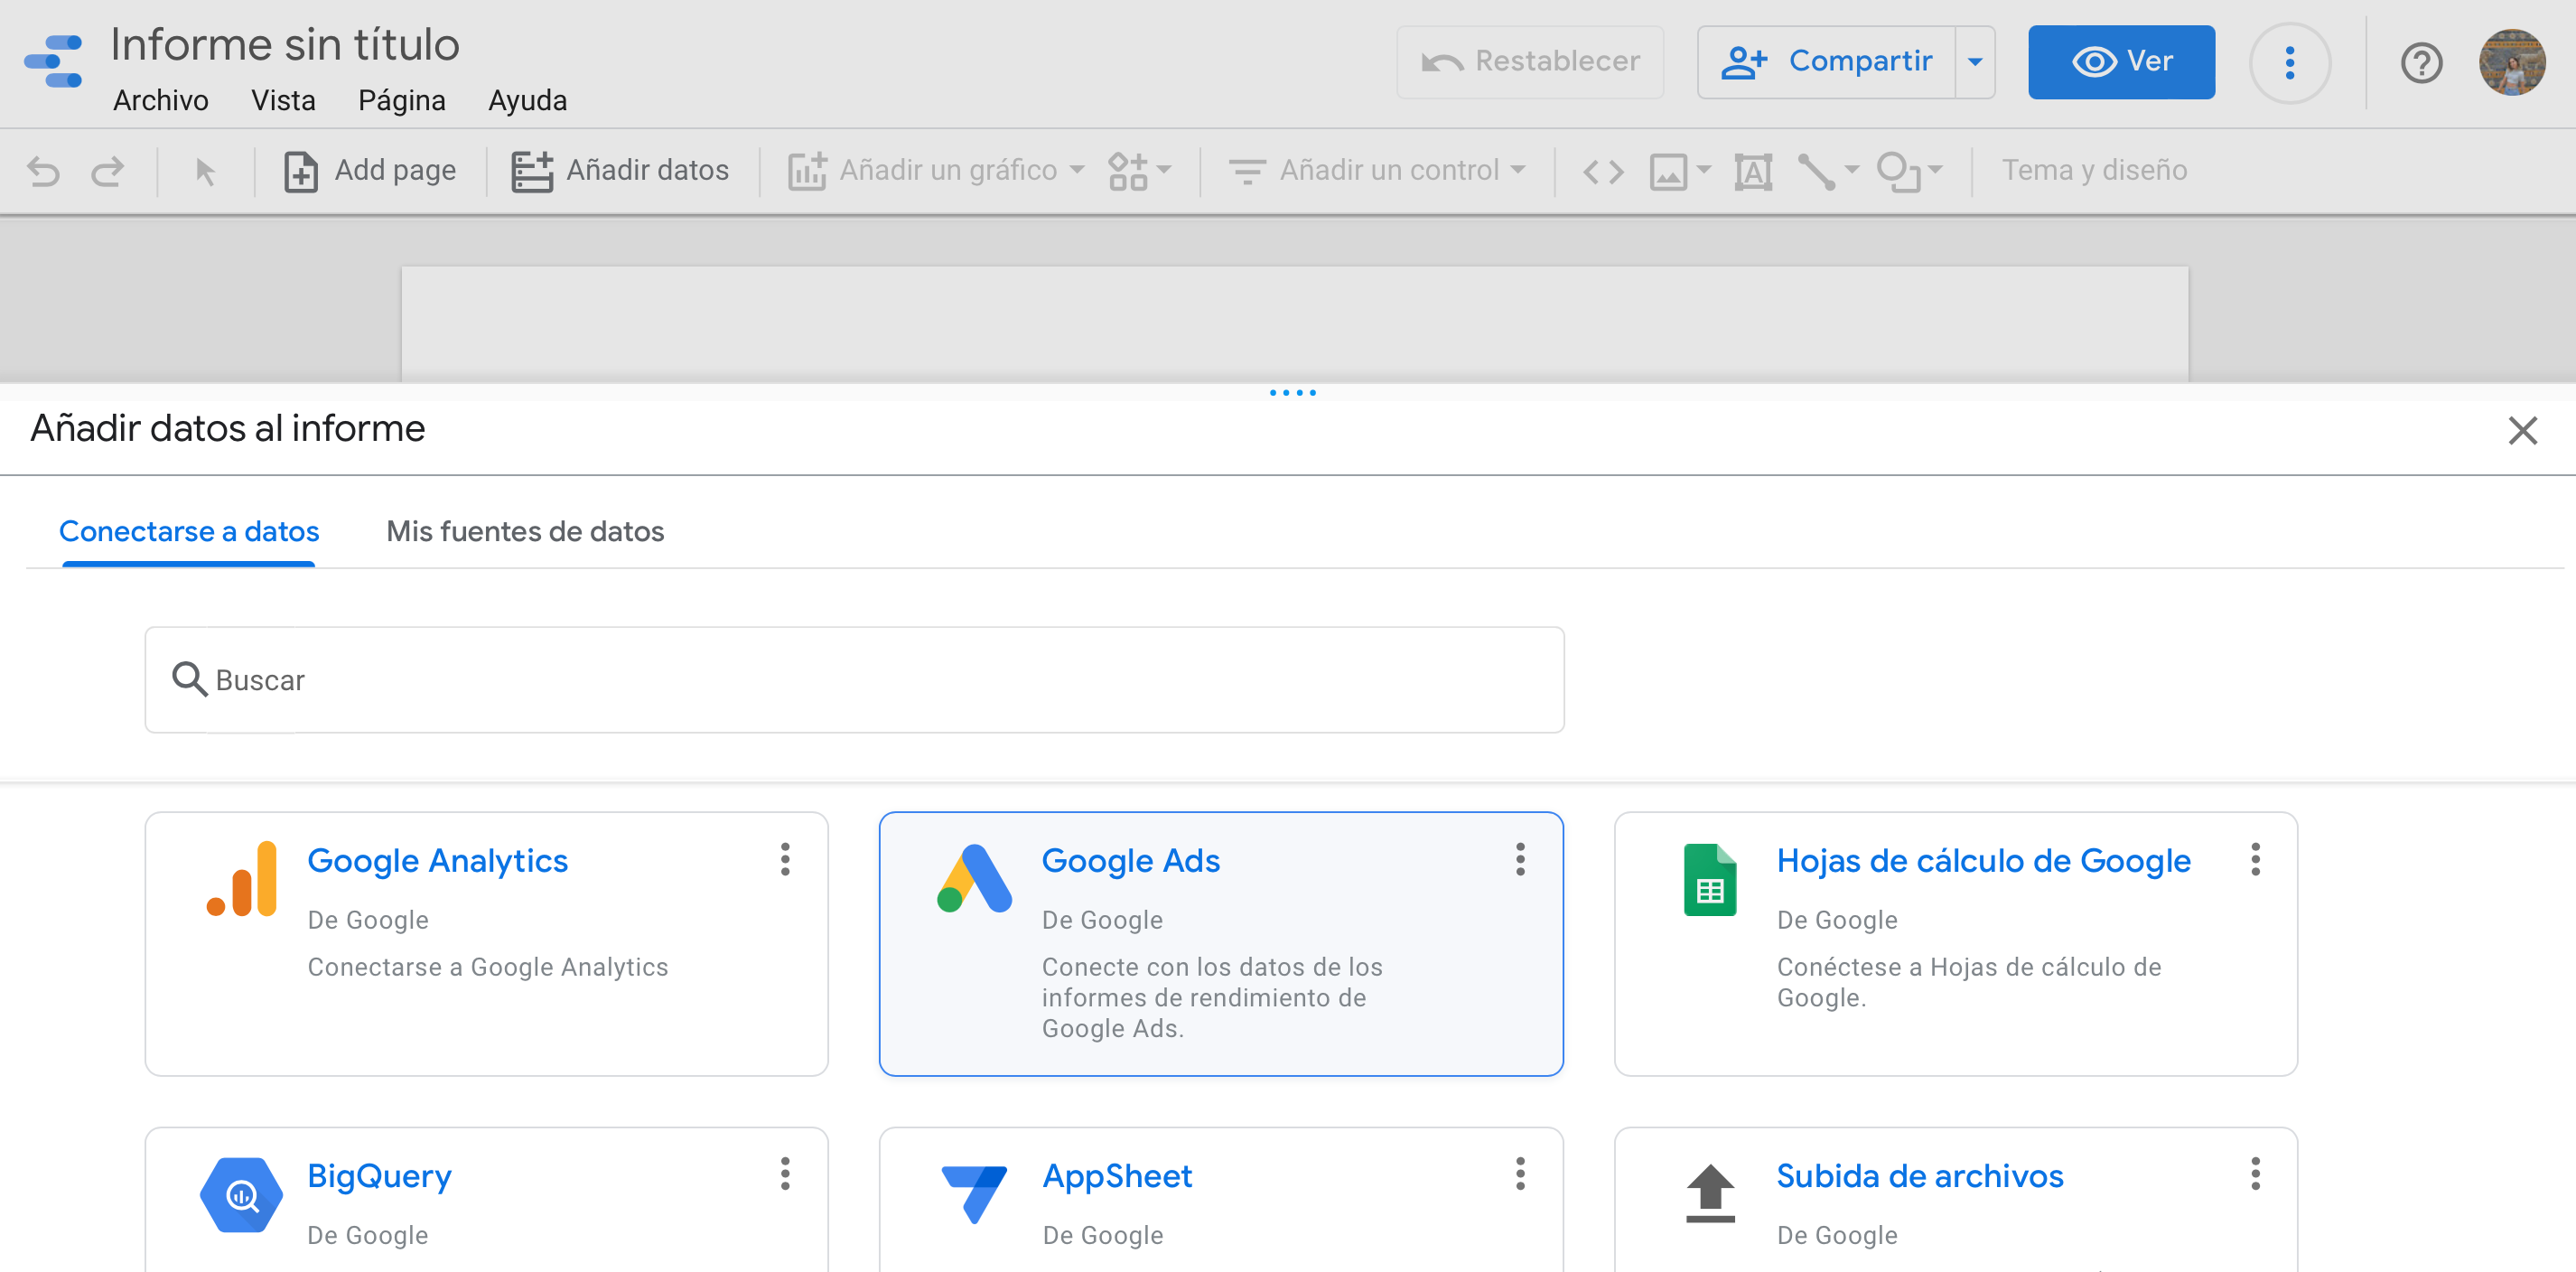
\includegraphics[width=10cm]{ds2}
\end{center}
\caption{Afegir dades a Data Studio}
\label{fig:ds2}
\end{figure}
\vspace{2mm}

Després podem canviar el nom d'aquesta pestanya particular en la visualització. Li donaré un nom representatiu de prodvalor per estat. Més enllà d'això, també podem establir un nom per a tota la visualització. Cridaré a aquesta mel de producció, i després premi guardar. I una vegada guardat aquest informe, podem seguir endavant i afegir una segona pestanya en la qual inclourem un gràfic diferent. Per al gràfic, ampliarem el menú de gràfics. Aquesta vegada inclourem un gràfic de sèries temporals suavitzades. Observarem que, per defecte, és la columna de l'any la que apareix en l'eix X, i és el valor de la producció de mel el que apareix en l'eix I. No obstant això, hi ha una línia separada per a cada estat. Si observa la configuració del gràfic, observarà que és la columna de l'any la que apareix com a dimensió principal, però també hi ha una columna de desglossament que apunta a l'estat. Això significa que sota el capó s'ha realitzat una operació d'agrupació per basada en els camps d'any i estat. A més, tingui en compte que les visualitzacions generades en Data Studio són interactives. Es pot obtenir informació addicional passant el ratolí per sobre de diferents punts del gràfic. No obstant això, mantinguem aquest gràfic simple i eliminem aquest camp de desglossament, la qual cosa ens dona un gràfic més simple i menys sorollós. Amb aquesta nova pestanya en el seu lloc, repetirem els passos que realitzem anteriorment establint un nou nom per a aquesta pestanya. La diré Valor de producció total en el temps. Assegura't que aquest gràfic s'ha guardat amb els canvis. I ara en cas que t'estiguis preguntant com pots accedir a aquesta visualització. Bé, pots copiar aquesta URL datastudio.google.com per a accedir a aquest servei. Navegaré a aquest enllaç en una nova pestanya. Això farà que aparegui el teu propi panell de control de Data Studio en el qual pots navegar a l'Explorador. I si els continguts estan ordenats en ordre descendent de temps, Producció de Mel hauria d'aparèixer en la part superior aquí. Quan es fa clic en això, és la mateixa visualització en la qual acabem de treballar. Per descomptat, podem confirmar-ho accedint a la segona pestanya. Efectivament, apareix el gràfic de sèries temporals. Cal tenir en compte que també podem compartir aquest informe amb altres usuaris. Amb això hem completat un ràpid cop d'ull a Data Studio i la seva integració amb BigQuery.

\newpage

\listoffigures


\end{document}
